\documentclass{book}

\title{Applied Computer Science}
\author{William John Holden}

\usepackage[utf8]{inputenc}
\usepackage{graphicx}
\usepackage{listings}
\usepackage{url}
\usepackage{geometry}
\usepackage{amsmath}
\usepackage{float}
\usepackage{amssymb}

%\usepackage{draftwatermark}
%\SetWatermarkScale{4}

% RSA
\usepackage{amsthm}
\usepackage{float}
\usepackage{textcomp}
\usepackage{gensymb}

% Binary
\usepackage{multicol}

% caesar
\usepackage{ulem}

% radio 
\usepackage{siunitx}

\usepackage[linktoc=all,hidelinks]{hyperref}

% style first used in Binary
\lstset{
  basicstyle=\ttfamily,
  columns=fullflexible,
  frame=single,
%  mathescape,  % removed in recursion
  xleftmargin=.5in,
  xrightmargin=.5in,
  captionpos=below
}

\begin{document}

\frontmatter
\maketitle
\tableofcontents

\chapter{To Do List}

\begin{center}
\begin{tabular}{c | c | c}
Chapter & Todo & Peer Review \\
\hline
1 & Complete rewrite in less conversational tone & -- \\
2 & Redo graphics. Show faster Union-Find algorithms using linked lists. & -- \\
3 & Cite EWD, RFC2453. Replace pseudocode with Java or C. & -- \\
4 & Show non-iterative algorithm to compute modular inverse  & -- \\
5 & Fix format and captions on code listings & -- \\
6 & Clear errors in bib on manpages & -- \\
7 & -- & -- \\
8 & Need Pankaj? Change image widths & -- \\
9 & Adjust text to fit listings on page & -- \\
10 & -- & DM \\
11 & \textit{Unfinished} & -- \\
12 & \textit{Unfinished} & -- \\
13 & -- &  \\
14 & -- & -- \\
15 & Add citations & -- \\
16 & \textit{Unfinished} & -- \\
17 & Use cleaner code from actual lecture & -- \\
18 & \textit{Unfinished} & -- \\
19 & \textit{Unfinished} & -- \\
\end{tabular}
\end{center}

A program listing somewhere might be missing.

Need to standardize indentation for all code listings.

Need to standardize use or non-use of section headings.

\mainmatter

\chapter{A Polish Calculator}

\section{A Polish Calculator}
Yesterday we built a Polish Calculator in JavaScript. Polish notation is interesting because it always uses \textit{prefix} notation instead of infix or postfix notation. In prefix notation, operators are written before operands. Our Polish Calculator is intentionally simple. The grammar supports only the four basic arithmetic operations ($+$, $-$, $*$, and $/$). Each of these functions are \textit{binary operators}, meaning they require exactly two parameters.

\section{Grammar}
In Extended Backus-Naur Form (EBNF), the grammar is:

\begin{lstlisting}
<expression> ::= <operator> (<expression> | <number>)
                 (<expression>|<number>)
<operator> ::= `+' | `-' | `*' | `/'
<number> ::= `-'? <digit>+ (`.' <digit>+)?
<digit> := `0' | `1' | `2' | `3' | `4' | `5' | `6' | `7' | `8' | `9'
\end{lstlisting}

The following inputs are not valid expressions in this grammar:

\begin{lstlisting}
+
+ 1
1
+ hello world
+ 1 1 1
\end{lstlisting}

\section{Implementation}

However, in our JavaScript program we spent no effort validating input. The program will still attempt to process any input with undefined results. Normally, production software should detect invalid input and use the language's exception-handling mechanisms to fail gracefully.

Our program first reads an expression from the \texttt{<input>} field using JavaScript's \texttt{document.getElementById} function. The expression breaks the input string into \textit{lexemes} using the \texttt{split} function, splitting the input string by spaces. Now we have an array of lexemes that we process as a \textit{queue}.

The queue is sent to the \texttt{calc} function. This function is \textit{recursive}, which means that it invokes itself. Many algorithms are recursive in nature; we will see this concept frequently.

The \texttt{calc} function retrieves and removes the lexeme at the head of the queue using the \texttt{shift} function. If the lexeme is an operator then the \texttt{calc} function will invoke itself twice to obtain the ``left'' and ``right'' operands, then calculate and and return the result. If the lexeme is not an operator then it is parsed as a number using JavaScript's \texttt{Number} constructor and returned as a value.

\begin{lstlisting}
function calc(queue) {
  if (queue.length === 0) return 0;

  var value = queue.shift();
  if (value === "+") {
    var left = calc(queue);
    var right = calc(queue);
    return left + right;
  } else if (value === "-") {
    var left = calc(queue);
    var right = calc(queue);
    return left - right;
  } else if (value === "*") {
    var left = calc(queue);
    var right = calc(queue);
    return left * right;
  } else if (value === "/") {
    var left = calc(queue);
    var right = calc(queue);
    return left / right;
  } else {
    return Number(value);
  }
}
\end{lstlisting}

(Note: in the program we wrote yesterday, we did not explicitly define a \textit{base case} telling the \texttt{calc} function what to do if the queue is empty.)

\section{Lambda Expressions}
The first implementation works, but it is inelegant. Is there a more abstract way to handle these operators? Yes - using \textit{lambda expressions} (typically known as \textit{arrow functions} in JavaScript).

A lambda expression is a function that is passed to another function as data. These functions are often \textit{anonymous}, meaning they are not explicitly named. The syntax, semantics, and structure for lambda expressions varies significantly among programming languages.

To easily manage our code as thought it were data, we introduce a useful data structure known as a \textit{map}. A map is simply a relation of key and value pairs.

Our program is thus shortened to:

\begin{lstlisting}
var operators = new Map();
operators.set("+", (left, right) => left + right);
operators.set("-", (left, right) => left - right);
operators.set("*", (left, right) => left * right);
operators.set("/", (left, right) => left / right);

function calc(queue) {
  if (queue.length === 0) return 0;

  var value = queue.shift();
  if (operators.has(value)) {
    return operators.get(value)(calc(queue), calc(queue));
  } else {
    return Number(value);
  }
}
\end{lstlisting}

We experimented with other techniques for compressing the code even further, but at the cost of readability. Generally speaking, beware of overly ``clever'' code. In the words of Brian Kernighan, 

\begin{quote}
Everyone knows that debugging is twice as hard as writing a program in the first place. So if you're as clever as you can be when you write it, how will you ever debug it?
\end{quote}

\section{Binary Trees}

We can visualize our grammar as a \textit{binary tree}. A binary tree is a data structure where abstract \textit{nodes} are related to zero, one, or two children. Only the \textit{root node} of a binary tree has no parent. A \textit{leaf node} has no children.

In our grammar, the root node and all intermediate nodes are always operators and leaves are always numeric values. Furthermore, a valid expression in our grammar must form a \textit{full} tree where each intermediate node has exactly two children.

A visualization for the expression \texttt{+ 7 * / 81 27 - 11 10} as a binary tree:

\begin{figure}[ht]
  \centering
  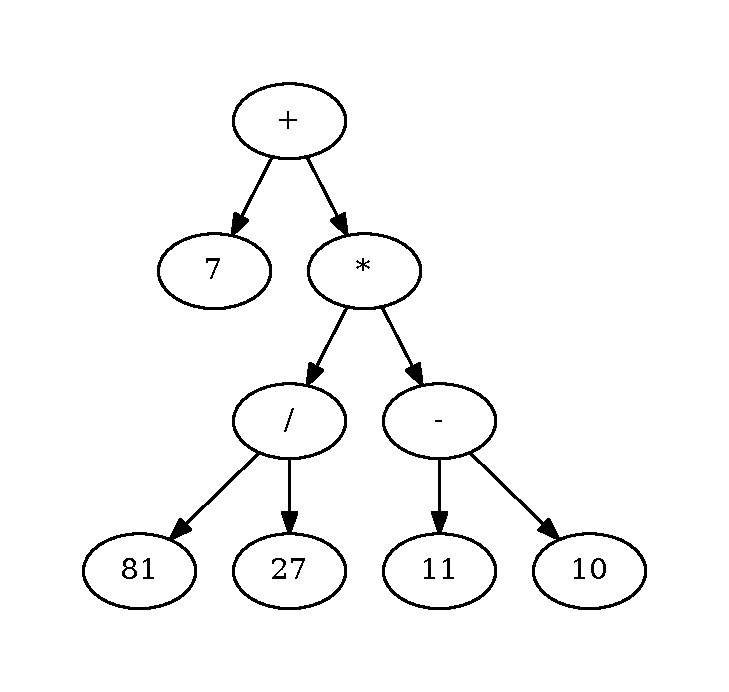
\includegraphics[width=\textwidth,height=.95\textheight,keepaspectratio]{figures/polish}
  \caption{\texttt{+ 7 * / 81 27 - 11 10} shown as a binary tree}
  \label{polish}
\end{figure}

\section{Food for thought}
We implemented a simple grammar for binary operators. Think about what would be required to:

\begin{enumerate}
\item Add an exponentiation operator, `\texttt{\^}'.
\item Support unary operators, such as a factorial (`\texttt{!}').
\item We ``overload'' the `\texttt{-}' operator to mean two different things: subtraction and negation. Once we support unary operators, will it be easy to give `\texttt{-}' two meanings?
\item Can we allow arbitrarily many arguments to our binary operators? For example, \texttt{+ 1 2 3}?
\item If we support $n$-ary operators, what does the expression \texttt{+ + 1 2 3 4 5 6} mean?
\item Suppose you extend your grammar to support parenthesis. Take a look at a programming language named Lisp.
\end{enumerate}

\chapter{Minimum Spanning Trees}

\section{Minimum Spanning Trees}

A \textit{graph} $G=(V,E)$ is an abstract combination of a vertex set $V$ and an edge set $E$ \cite{rosen2003discrete}. A \textit{set} is an unsorted collection of unique elements. An \textit{edge} is a relation $(u,v)$ between two vertices $u$ and $v$, so an edge set $E$ contains all relations between vertices in the vertex set. Rules for edges will depend on the application; some graphs may allow edges to be weighted or unweighted, directed or undirected, parallel, or self-referential (e.g., an edge $(u,u)$ that relates a vertex to itself).

Figure \ref{spannABC} visualizes an unweighted and undirected graph $G=(V,E)$ where $V=\{a,b,c\}$ and $E=\{(a,b), (b,c), (c,c), (a,c), (a,c)\}$.

\begin{figure}[ht]
\centering
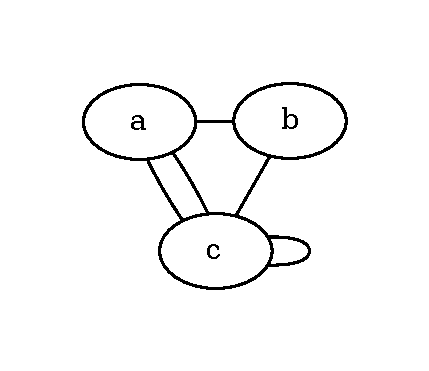
\includegraphics[height=2in]{figures/spanning-abc}
\caption{An unweighted, undirected, cyclic graph}
\label{spannABC}
\end{figure}

The graph shown in figure \ref{spannABC} is cyclic, which means that it contains two loops, one around $a \to b \to c$ and another at $c \to c$.

\begin{figure}[ht]
\centering
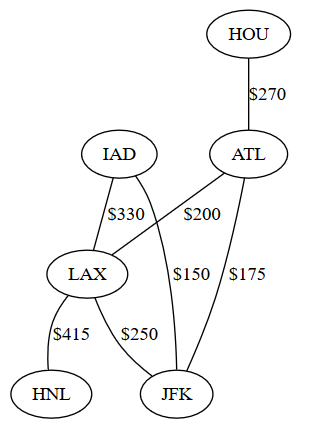
\includegraphics[height=2in]{ch-spann/02}
\caption{A weighted, undirected, cyclic graph}
\label{2}
\end{figure}

Edges can be weighted. Figure \ref{2} shows a hypothetical airline. The vertex set contains airports and the edge set represents flights connecting airports. Each edge is weighted by the dollar cost of the flight.

A \textit{tree} is an acyclic graph. A \textit{spanning tree} is an acyclic graph where each vertex is a member of the same \textit{component}. The graph shown in figure \ref{3} is not a spanning tree because there exists no path from any vertex in the left component to any vertex in the right component. However, each component is a tree because the subgraphs are acyclic.

\begin{figure}[ht]
\centering
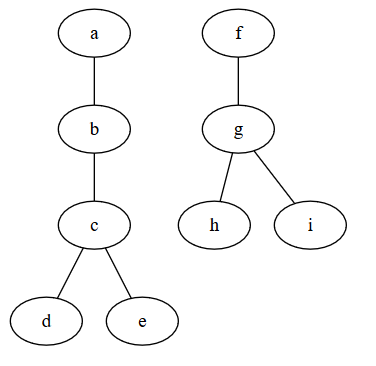
\includegraphics[height=2in]{ch-spann/03}
\caption{This graph contains two components, and each component is a tree}
\label{3}
\end{figure}

A \textit{minimum spanning tree} (MST) is a spanning tree with the minimum possible sum of edge weights \cite{rosen2003discrete}. Figure \ref{4} shows that it is possible to construct more than one MST for a graph. Formally, the edge set $T$ of an MST is a connected acyclic subset $T \subseteq E$ minimizing the total weight \cite{cormen2001introduction}:

\begin{equation}
w(T) = \sum_{(u,v) \in T}{w(u,v)}
\end{equation}

\begin{figure}[ht]
\centering
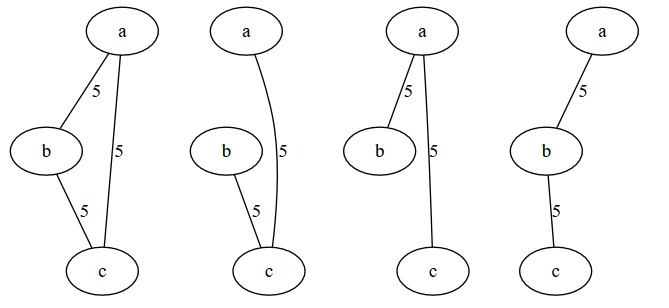
\includegraphics[width=.75\textwidth]{ch-spann/04}
\caption{A graph may have many minimum spanning trees}
\label{4}
\end{figure}

An example application for a minimum spanning tree is the ``muddy roads problem.'' Imagine a city with no paved roads. The leaders of this city wish to connect each building at the lowest cost. To do so, the architect can use a minimum spanning tree to connect the city while minimizing the overall weight of the connected graph.

Two well-known algorithms for computing the minimum spanning tree are Kruskal's algorithm and Prim's algorithm. Both are \textit{greedy} algorithms. In greedy algorithms, a locally optimal choice can be used at each step to arrive at a globally optimal solution \cite{cormen2001introduction}.

\section{Kruskal's algorithm}

Kruskal's algorithm places each edge of $E$ into a priority queue $Q$. The algorithm extracts the minimum weight edge $(u,v)$ from $Q$ and checks if adding $(u,v)$ to the MST $T$ would form a loop. If no cycle occurs then the edge is added to $T$ and the algorithm continues until $|T|= |V|-1$.

What happens if two edges have equal weight? Kruskal's algorithm does not specifically define what to do, but it turns out that it does not matter. Either edge can be used to build an MST. Often, the behavior of the priority queue's \texttt{Extract-Min} implementation will determine which of two equal-cost edges is presented first.

Figures 5 through 11 show an execution of Kruskal's algorithm. The blue edges are those added to the MST $T$.

\newgeometry{left=1in,bottom=1in}
\begin{figure}[ht]
\centering
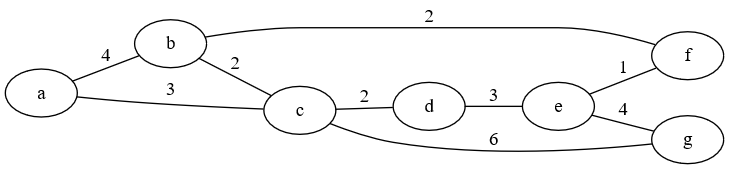
\includegraphics[width=3.4in]{ch-spann/kruskal-1}
\label{kruskal1}
\caption{Initial graph to find an MST $T$ with Kruskal's algorithm}

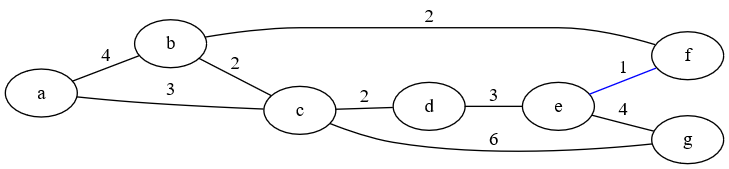
\includegraphics[width=3.4in]{ch-spann/kruskal-2}
\label{kruskal2}
\caption{Add $(e,f)$ to $T$}

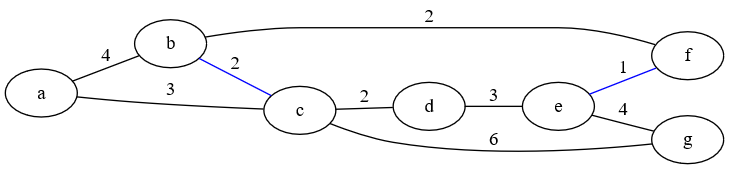
\includegraphics[width=3.4in]{ch-spann/kruskal-3}
\label{kruskal3}
\caption{Add $(b,c)$ to $T$}

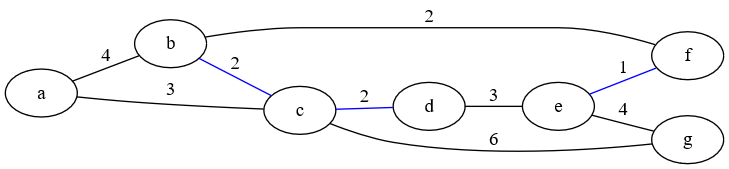
\includegraphics[width=3.4in]{ch-spann/kruskal-4}
\label{kruskal4}
\caption{Add $(c,d)$ to $T$}

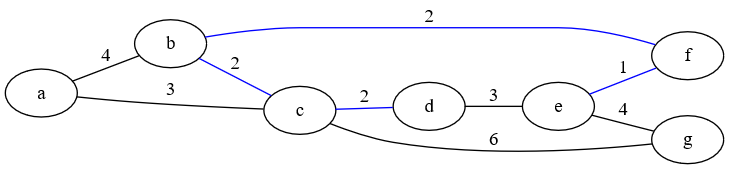
\includegraphics[width=3.4in]{ch-spann/kruskal-5}
\label{kruskal5}
\caption{Add $(b,f)$ to $T$}

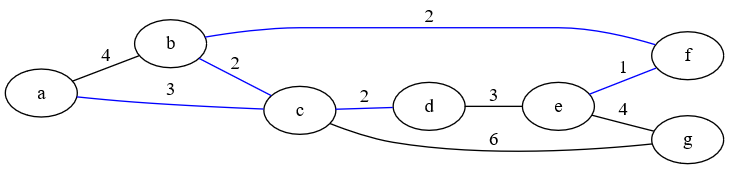
\includegraphics[width=3.4in]{ch-spann/kruskal-6}
\label{kruskal6}
\caption{Add $(a,c)$ to $T$}

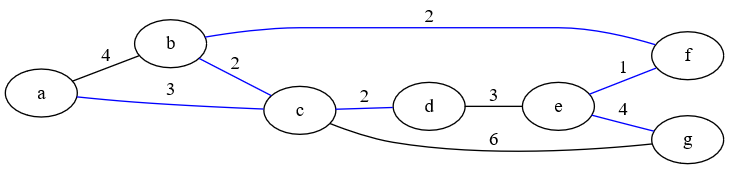
\includegraphics[width=3.4in]{ch-spann/kruskal-7}
\label{kruskal7}
\caption{Skip $(d,e)$ and add $(e,g)$ to $T$}
\end{figure}
\restoregeometry

A program available at \url{https://wjholden.com/Kruskal.jar} (source \url{https://wjholden.com/MinimumSpanningTree.java}) can be used to visualize Kruskal's algorithm. Edges in this program are weighted by pixel distance on the screen.

\begin{figure}[h]
\centering
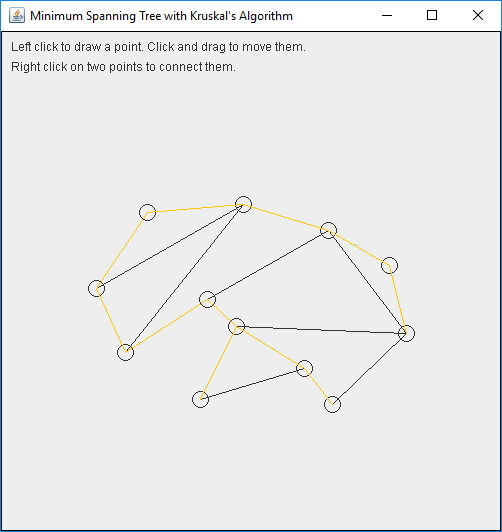
\includegraphics[height=2in]{ch-spann/kruskal-app}
\label{kruskal-app}
\caption{Visualization of Kruskal's algorithm with edges weighted by distance}
\end{figure}

\section{Union-Find}
Kruskal's algorithm only inserts edges to $T$ if they do not introduce a cycle. The presence of a cycle can be detected using the Union-Find algorithm for disjoint sets \cite{cormen2001introduction}.

Union-Find initializes with each vertex assigned to a separate component. The components for each vertex are joined as Kruskal's algorithm connects vertices by adding edges. Edges are only added to the MST when the vertices are in disjoint components.

The following steps illustrate how Union-Find was used to perform Kruskal's algorithm in figures 5 through 11:

\begin{enumerate}

\item Initialize each vertex in disjoint components $\{a\}$, $\{b\}$, $\{c\}$, $\{d\}$, $\{e\}$, $\{f\}$, and $\{g\}$.

\item Adding $(e,f)$ to $T$ causes a union of their components $\{e\} \cup \{f\} = \{e,f\}$. The components become $\{a\}$, $\{b\}$, $\{c\}$, $\{d\}$, $\{e,f\}$, and $\{g\}$.

\item Add $(b,c)$ to $T$ and update the components for $\{b\} \cup \{c\} = \{b,c\}$ creating $\{a\}$, $\{b,c\}$, $\{d\}$, $\{e,f\}$, and $\{g\}$.

\item Adding $(c,d)$ to the MST does not create a cycle because $\{b,c\} \cap \{d\} = \emptyset$. Add $(c,d)$ to $T$ and the disjoint sets become $\{a\}$, $\{b,c,d\}$, $\{e,f\}$, $\{g\}$.

\item $(b,f) \cup T$ results in $\{b,c,d\} \cup \{e,f\}$. The disjoint sets are updated as $\{a\}$, $\{b,c,d,e,f\}$, and $\{g\}$.

\item $(a,c) \cup T$ and get $\{a,b,c,d,e,f\}$ and $\{g\}$.

\item At this point we might have been tempted to add $(d,e)$ because the weight is 3, but vertices $d$ and $e$ are already members of the same component $\{a,b,c,d,e,f\}$. If we added $(d,e)$ we would create a cycle, so instead we skip $(d,e)$. $(e,g) \cup T$ completes the MST with single connected component $\{a,b,c,d,e,f,g\}$.

\end{enumerate}

\section{Prim's algorithm}

Prim's algorithm is another greedy algorithm for computing an MST. Prim's algorithm begins with some starting vertex $u$ and adds each of $u$'s edges to a priority queue $Q$. Extract the minimum weight edge $(u,v)$ and add each of $v$'s edges to $Q$. Extract the minimum weight edge again. If the extracted edge does not produce a cycle then add its edges to $Q$ and continue until the graph is fully connected.

The most ``expensive'' operations in both Kruskal's algorithm Prim's algorithm are in the priority queue. There are many data structures and associated algorithms for managing priority queues. Various approaches to managing queues have unequal performance.

Figures 13 through 19 illustrate Prim's algorithm using the same graph as before, highlighting both the edges in $T$ and the vertices visited in blue.

\newgeometry{left=1.5in,bottom=1.5in}
\begin{figure}[ht]
\centering
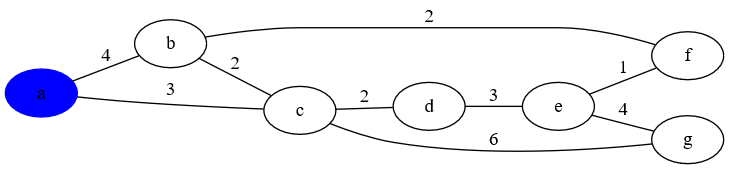
\includegraphics[width=3.4in]{ch-spann/prim1}
\label{prim1}
\caption{Initial graph to use Prim's algorithm beginning at vertex $a$}

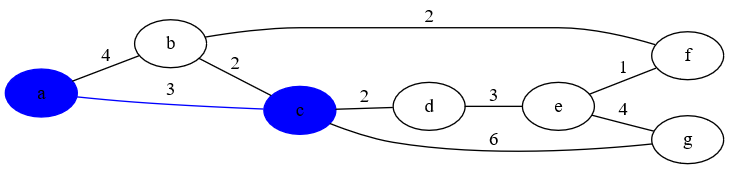
\includegraphics[width=3.4in]{ch-spann/prim2}
\label{prim2}
\caption{Add $(a,c)$ to $T$}

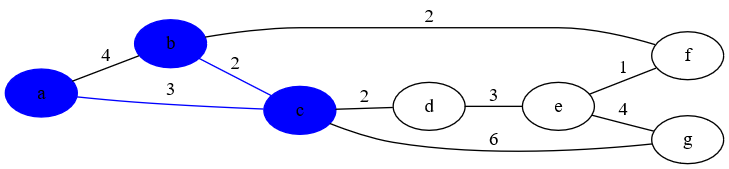
\includegraphics[width=3.4in]{ch-spann/prim3}
\label{prim3}
\caption{Add $(b,c)$ to $T$}

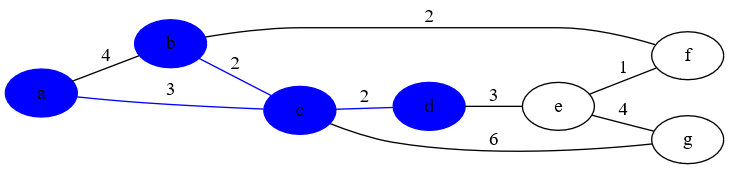
\includegraphics[width=3.4in]{ch-spann/prim4}
\label{prim4}
\caption{Add $(c,d)$ to $T$}

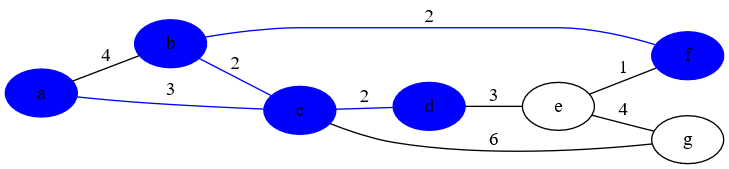
\includegraphics[width=3.4in]{ch-spann/prim5}
\label{prim5}
\caption{Add $(b,f)$ to $T$}

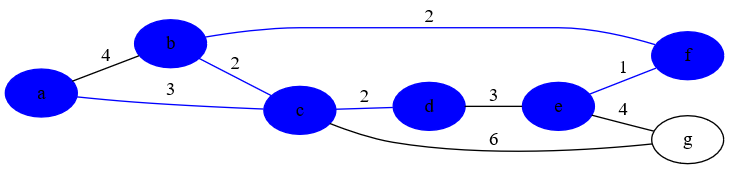
\includegraphics[width=3.4in]{ch-spann/prim6}
\label{prim6}
\caption{Add $(e,f)$ to $T$ because it has the lowest weight}

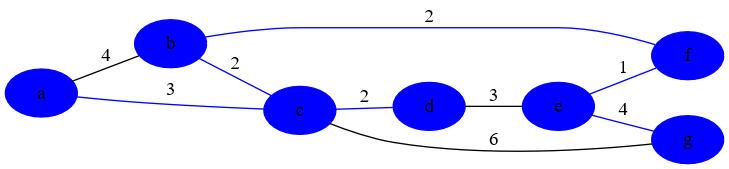
\includegraphics[width=3.4in]{ch-spann/prim7}
\label{prim7}
\caption{Skip $(d,e)$ and add $(e,g)$ to $T$}
\end{figure}
\restoregeometry

\section{Spanning Tree Protocol}

Perhaps the best known practical application for MST's is Radia Perlman's Spanning Tree Protocol (STP) \cite{Perlman:1985:ADC:318951.319004}. STP creates a loop-free network topology for Ethernet bridges with no configuration by unblocking only the lowest-cost path to the root bridge.

A \textit{learning bridge} or \textit{switch} records the source address of a Ethernet frame and stores it in the MAC Address table. If the destination address is present in the MAC address table then the frame will be forwarded only to that port. If the destination is not known or is a broadcast address then the frame will be ``flooded'' out of each port except the source port \cite{perlman2000interconnections}.

The broadcasting and flooding of Ethernet frames allows devices to discover one another automatically with no configuration. The protocol allows bridges to separate collision domains, preventing signals from jamming one another on a shared physical media. However, Ethernet does not feature \textit{time to live} (TTL) or \textit{hop count} fields like Internet Protocol. To prevent loops, Ethernet uses the Spanning Tree Protocol to unblock an acyclic subset of the network topology.

A program available at \url{https://github.com/wjholden/NetViz} can be used to visualize the behavior of frames flooded between switches.

\begin{figure}[ht]
\centering
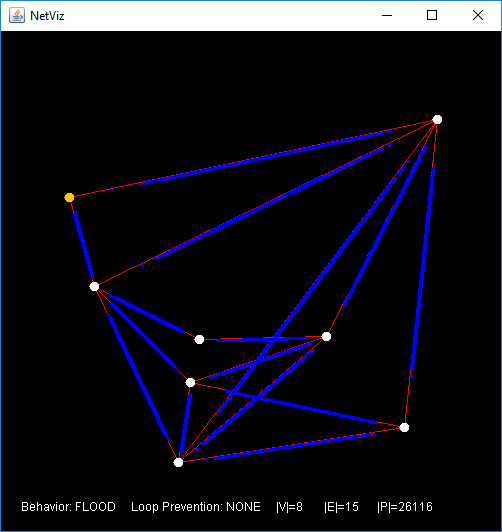
\includegraphics[height=2in]{ch-spann/netviz}
\label{netviz}
\caption{Visualization of broadcast storms created by flooding}
\end{figure}

\chapter{Dijkstra's Algorithm}

\section{Paths in a Graph}
A graph $G=(V,E)$ can contain many \textit{paths} that transitively connect vertices in the same component. For example, in a graph $V=\{a,b,c,d\}$ and $E=\{(a,b),(b,d),(a,c),(c,d)\}$ there exist two paths from $a$ to $d$: $a,b,d$ and $a,c,d$. A path should not contain a vertex more than once.

\section{Breadth-First Search}
Recall that the edges in a graph may be weighted or unweighted, directed or undirected. Breadth-First Search (BFS) is a simple algorithm for finding the shortest path in graphs containing only \textit{unweighted} edges \cite{cormen2001introduction}. BFS begins at some starting vertex $s$ and traverses the graph outwards by concentric frontiers.

\begin{lstlisting}[caption={Breadth-First Search in pseudocode}, captionpos=b, mathescape, xleftmargin=.25in, xrightmargin=.25in]
Breadth-First-Search (Graph $G=(V,E)$, Vertex $s$) {
  assume $s \in V$
  $Q = \{ s \}$ // queue of vertices to process
  $S = \emptyset$ // set of vertices already discovered

  while $Q \ne \emptyset$ {
    Vertex $u = Q$.Dequeue()
    $S = S \cup \{u\}$
    for each Vertex $v$ where $\exists v [ (u,v) \in E ] \wedge v \notin S$ {
      $Q$.Enqueue($v$)
    }
  }
}
\end{lstlisting}

This example BFS implementation is different from that shown on page 595 of CLRS.

Figure \ref{bfs} shows an example Breadth-First traversal of a graph. Each vertex is colored by distance from $a$. The distance of the shortest path ($\delta$) from $a$ to $b$ and $c$ is $1$.

\begin{figure}[ht]
\centering
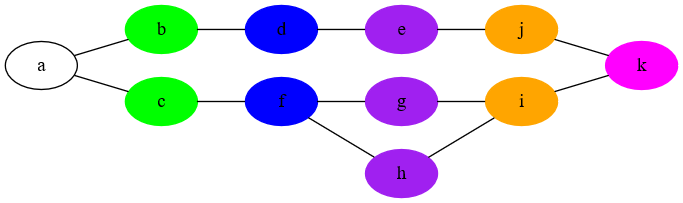
\includegraphics[width=\textwidth]{ch-dijkstra/bfs}
\caption{BFS traversal of an unweighted graph}
\label{bfs}
\end{figure}

\begin{align*}
\delta(a,a) = 0 \\
\delta(a,b) = \delta(a,c) = 1 \\
\delta(a,d) = \delta(a,f) = 2 \\
\delta(a,e) = \delta(a,g) = \delta(a,h) = 3 \\
\delta(a,j) = \delta(a,i) = 4 \\
\delta(a,k) = 5
\end{align*}

The Routing Information Protocol (RIP) uses a simple hop count as its metric to forward traffic through the optimal path. One could use BFS to model a RIP topology.

\section{Dijkstra's Algorithm}

Though RIP is simple to configure and understand, it can lead to submaximal network performance. If a network has multiple paths from a source to a destination then the router will select the path with the fewest edges, not necessarily the path with the smallest aggregate edge weight.

Dijkstra's algorithm can compute the shortest path tree, starting at some starting vertex $s$, based on minimal path weight. The Open Shortest Path First (OSPF) routing protocol uses Dijkstra's algorithm with a complete topology table to compute the lowest cost path based on \textit{cost}. The cost of a link is normally a function of bandwidth but can be manually configured.

Dijkstra's algorithm is \textit{greedy} and makes the locally optimal solution in order to construct a globally optimal solution. The algorithm constructs a priority queue of vertices in the graph where the priority is keyed on aggregate distance, $\delta$. The distance to each vertex is initialized as $\infty$, except for the starting vertex $s$ which obviously has a distance of 0 to itself ($\delta(s,s)=0$). From there, the algorithm extracts the vertex from the queue with the minimum total distance. Extracted vertices are \textit{relaxed}. Relaxing a vertex implies that the shortest path to that vertex has been found. Distances to each vertex adjacent $v$ to the relaxed vertex $u$ are updated if and only if $\delta(s,u)+w(u,v)<\delta(s,v)$. The algorithm halts when all vertices are relaxed.

\begin{lstlisting}[caption={Dijkstra's algorithm in pseudocode}, captionpos=b, mathescape, xleftmargin=.25in, xrightmargin=.25in]
Dijkstra-Shortest-Path (Graph $G=(V,E)$, Vertex $s$) {
  assume $s \in V$
  $Q$ = New-Priority-Queue(priority $= \delta$) // a priority queue of vertices to discover
  $V$.Add-Attributes($\delta$, visited, parent) // $\delta$ is distance from $s$
  
  for each Vertex $v \in V$ except $s$ {
    $Q$.Enqueue($v$, $\delta = \infty$, visited $= F$, parent $= \emptyset$)
  }
  
  $s.\delta = 0$ // initialize $s$ with zero distance from itself
  
  while $Q \ne \emptyset$ {
    Vertex $u = Q$.Dequeue()
    for each Vertex $v \in V$ where $v$.relaxed $= F \wedge \exists v[(u,v) \in E] $ {
      if ($v.\delta > u.\delta + w(u,v)$) {
        $v.\delta = u.\delta + w(u,v)$
        $v$.parent $= u$
      }
    }
    $u$.visited $= T$
  }
}
\end{lstlisting}

Consider the below graph shown in figure \ref{spf0}. 

\begin{figure}[H]
\centering
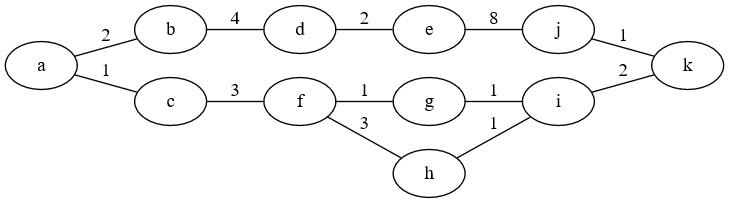
\includegraphics[width=\textwidth]{ch-dijkstra/spf0}
\caption{A weighted, undirected graph}
\label{spf0}
\end{figure}

To run Dijkstra's algorithm, starting at vertex $a$, initialize a map of vertices and distances from $a$. It is already known that $\delta(a,a)=0$. The distance to each other vertex is initialized as $\infty$.

\begin{table}[H]
\centering
\begin{tabular}{ | c | c | c | c | c | c | c | c | c | c | c | c | }
\hline
 & $a$ & $b$ & $c$ & $d$ & $e$ & $f$ & $g$ & $h$ & $i$ & $j$ & $k$ \\
 \hline
 distance & 0 & $\infty$ & $\infty$ & $\infty$ & $\infty$ & $\infty$ & $\infty$ & $\infty$ & $\infty$ & $\infty$ & $\infty$ \\
 \hline
 parent & $\emptyset$ & $\emptyset$ & $\emptyset$ & $\emptyset$ & $\emptyset$ & $\emptyset$ & $\emptyset$ & $\emptyset$ & $\emptyset$ & $\emptyset$ & $\emptyset$ \\
 \hline
 relaxed & 0 & 0 & 0 & 0 & 0 & 0 & 0 & 0 & 0 & 0 & 0 \\
 \hline
\end{tabular}
\caption{Initial distances, parent nodes, and relaxation state}
\label{initial}
\end{table}

With the data structure shown in table \ref{initial} initialized, Dijkstra's algorithm will always \textit{relax} the vertex with the lowest distance, $u$. Relaxing an edge means that the algorithm will consider each of $u$'s adjacent edges, $(u,v)$. If $\delta(s, u) + w(u,v)$ is less than the value recorded in the table then $u$ provides a better path than what was previously recorded. Both the parent and distance values for each $v$ are updated and $u$ is marked relaxed. Once a vertex has been relaxed then $\delta(s,u)$ has been found; the algorithm need not visit $u$ again.

Figure \ref{spf1} shows the first relaxation pass on the graph. with $s=a$, the distances and parent pointers to update are for vertices $b$ and $c$.

\begin{figure}[H]
\centering
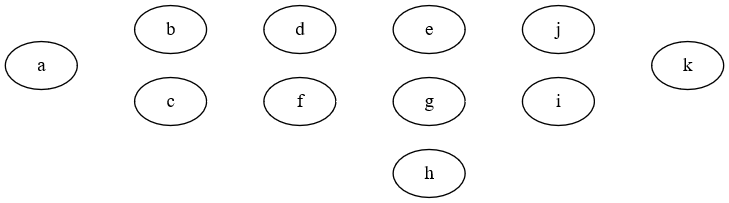
\includegraphics[width=.75\textwidth]{ch-dijkstra/spf1}
  \begin{tabular}{ | c | c | c | c | c | c | c | c | c | c | c | c | }
  \hline
   & $a$ & $b$ & $c$ & $d$ & $e$ & $f$ & $g$ & $h$ & $i$ & $j$ & $k$ \\
   \hline
   distance & 0 & 2 & 1 & $\infty$ & $\infty$ & $\infty$ & $\infty$ & $\infty$ & $\infty$ & $\infty$ & $\infty$ \\
   \hline
   parent & $\emptyset$ & $a$ & $a$ & $\emptyset$ & $\emptyset$ & $\emptyset$ & $\emptyset$ & $\emptyset$ & $\emptyset$ & $\emptyset$ & $\emptyset$ \\
   \hline
   relaxed & 1 & 0 & 0 & 0 & 0 & 0 & 0 & 0 & 0 & 0 & 0 \\
   \hline
  \end{tabular}
\caption{At initialization the only known shortest path is $\delta(a,a)=0$}
\label{spf1}
\end{figure}

The algorithm next relaxes $c$ because it has the lowest distance of any vertices where the distance from $a$ is not known. It is now known $\delta(a,f) \le \delta(a,c) + \delta(c,f) = 1 + 3 = 4$. It is obvious from the figure that indeed $\delta(a,f) = 4$, but if there existed an edge $(b,f)$ with $w(b,f)=1$ then $\delta(a,f)$ would be less than the candidate value of 4. It is not uncommon for Dijkstra's algorithm to \textit{backtrack} by updating distance and parent values as better paths are discovered.

\begin{figure}[H]
\centering
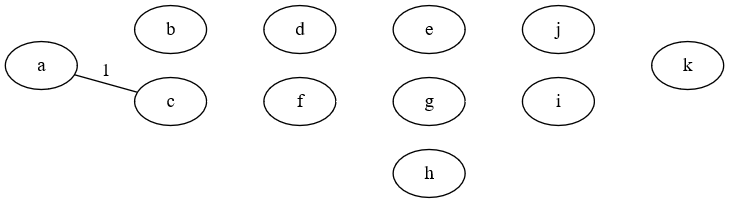
\includegraphics[width=.75\textwidth]{ch-dijkstra/spf2}
  \begin{tabular}{ | c | c | c | c | c | c | c | c | c | c | c | c | }
  \hline
   & $a$ & $b$ & $c$ & $d$ & $e$ & $f$ & $g$ & $h$ & $i$ & $j$ & $k$ \\
   \hline
   distance & 0 & 2 & 1 & $\infty$ & $\infty$ & 4 & $\infty$ & $\infty$ & $\infty$ & $\infty$ & $\infty$ \\
   \hline
   parent & $\emptyset$ & $a$ & $a$ & $\emptyset$ & $\emptyset$ & $c$ & $\emptyset$ & $\emptyset$ & $\emptyset$ & $\emptyset$ & $\emptyset$ \\
   \hline
   relaxed & 1 & 0 & 1 & 0 & 0 & 0 & 0 & 0 & 0 & 0 & 0 \\
   \hline
  \end{tabular}
\caption{Relaxing $c$ implies that $\delta(a,c)=1$ is globally optimal}
\label{spf2}
\end{figure}

Next, relax vertex $b$.

\begin{figure}[H]
\centering
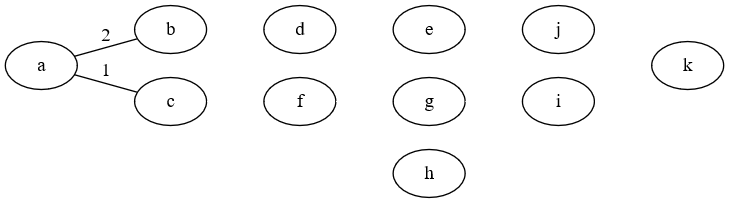
\includegraphics[width=.75\textwidth]{ch-dijkstra/spf3}
  \begin{tabular}{ | c | c | c | c | c | c | c | c | c | c | c | c | }
  \hline
   & $a$ & $b$ & $c$ & $d$ & $e$ & $f$ & $g$ & $h$ & $i$ & $j$ & $k$ \\
   \hline
   distance & 0 & 2 & 1 & 6 & $\infty$ & 4 & $\infty$ & $\infty$ & $\infty$ & $\infty$ & $\infty$ \\
   \hline
   parent & $\emptyset$ & $a$ & $a$ & $b$ & $\emptyset$ & $c$ & $\emptyset$ & $\emptyset$ & $\emptyset$ & $\emptyset$ & $\emptyset$ \\
   \hline
   relaxed & 1 & 1 & 1 & 0 & 0 & 0 & 0 & 0 & 0 & 0 & 0 \\
   \hline
  \end{tabular}
\caption{Relax $b$. $\delta(a,b)=2$}
\label{spf3}
\end{figure}

Relax $f$.

\begin{figure}[H]
\centering
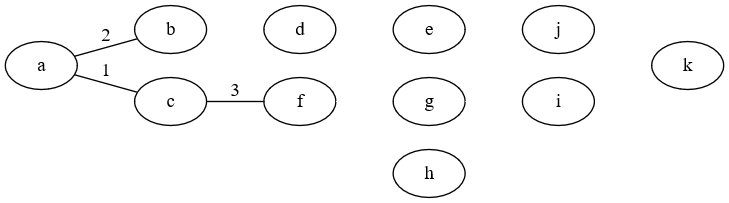
\includegraphics[width=.75\textwidth]{ch-dijkstra/spf4}
  \begin{tabular}{ | c | c | c | c | c | c | c | c | c | c | c | c | }
  \hline
   & $a$ & $b$ & $c$ & $d$ & $e$ & $f$ & $g$ & $h$ & $i$ & $j$ & $k$ \\
   \hline
   distance & 0 & 2 & 1 & 6 & $\infty$ & 4 & 5 & 7 & $\infty$ & $\infty$ & $\infty$ \\
   \hline
   parent & $\emptyset$ & $a$ & $a$ & $b$ & $\emptyset$ & $c$ & $f$ & $f$ & $\emptyset$ & $\emptyset$ & $\emptyset$ \\
   \hline
   relaxed & 1 & 1 & 1 & 0 & 0 & 1 & 0 & 0 & 0 & 0 & 0 \\
   \hline
  \end{tabular}
\caption{Relax $f$. $\delta(a,f)=\delta(a,c)+\delta(c,f)=1+3=4$}
\label{spf4}
\end{figure}

Relax $g$.

\begin{figure}[H]
\centering
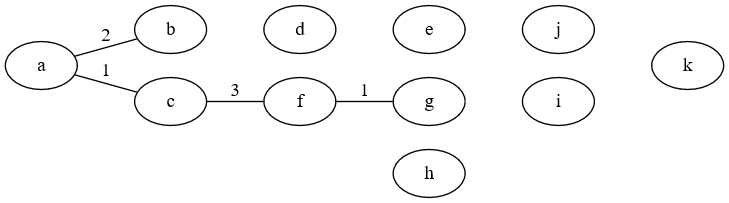
\includegraphics[width=.75\textwidth]{ch-dijkstra/spf5}
  \begin{tabular}{ | c | c | c | c | c | c | c | c | c | c | c | c | }
  \hline
   & $a$ & $b$ & $c$ & $d$ & $e$ & $f$ & $g$ & $h$ & $i$ & $j$ & $k$ \\
   \hline
   distance & 0 & 2 & 1 & 6 & $\infty$ & 4 & 5 & 7 & 6 & $\infty$ & $\infty$ \\
   \hline
   parent & $\emptyset$ & $a$ & $a$ & $b$ & $\emptyset$ & $c$ & $f$ & $f$ & $g$ & $\emptyset$ & $\emptyset$ \\
   \hline
   relaxed & 1 & 1 & 1 & 0 & 0 & 1 & 1 & 0 & 0 & 0 & 0 \\
   \hline
  \end{tabular}
\caption{Relax $g$. $\delta(a,g) = \delta(a,f) + \delta(f,g) = 4+1=5$}
\label{spf5}
\end{figure}

Based on this table, $\delta(a,d)=\delta(a,i)=6$. Select either vertex to continue finding shortest paths. It is not uncommon for a graph to contain equal-cost paths. In this case, relax $d$.

\begin{figure}[H]
\centering
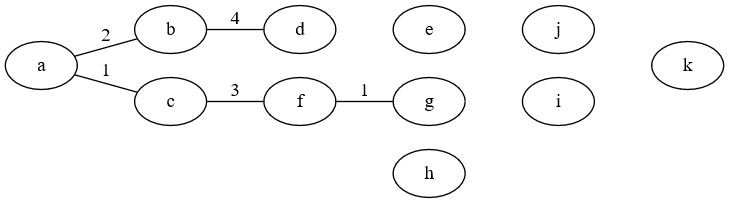
\includegraphics[width=.75\textwidth]{ch-dijkstra/spf6}
  \begin{tabular}{ | c | c | c | c | c | c | c | c | c | c | c | c | }
  \hline
   & $a$ & $b$ & $c$ & $d$ & $e$ & $f$ & $g$ & $h$ & $i$ & $j$ & $k$ \\
   \hline
   distance & 0 & 2 & 1 & 6 & 8 & 4 & 5 & 7 & 6 & $\infty$ & $\infty$ \\
   \hline
   parent & $\emptyset$ & $a$ & $a$ & $b$ & $d$ & $c$ & $f$ & $f$ & $g$ & $\emptyset$ & $\emptyset$ \\
   \hline
   relaxed & 1 & 1 & 1 & 1 & 0 & 1 & 1 & 0 & 0 & 0 & 0 \\
   \hline
  \end{tabular}
\caption{Relax $d$. $\delta(a,d) = \delta(a,b) + \delta(b,d) = 6$}
\label{spf6}
\end{figure}

Relax $i$.

\begin{figure}[H]
\centering
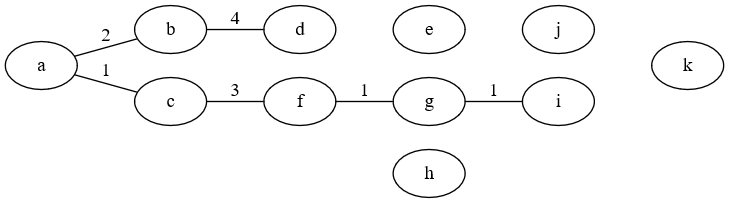
\includegraphics[width=.75\textwidth]{ch-dijkstra/spf7}
  \begin{tabular}{ | c | c | c | c | c | c | c | c | c | c | c | c | }
  \hline
   & $a$ & $b$ & $c$ & $d$ & $e$ & $f$ & $g$ & $h$ & $i$ & $j$ & $k$ \\
   \hline
   distance & 0 & 2 & 1 & 6 & 8 & 4 & 5 & 7 & 6 & $\infty$ & 8 \\
   \hline
   parent & $\emptyset$ & $a$ & $a$ & $b$ & $d$ & $c$ & $f$ & $f$ & $g$ & $\emptyset$ & $i$ \\
   \hline
   relaxed & 1 & 1 & 1 & 1 & 0 & 1 & 1 & 0 & 1 & 0 & 0 \\
   \hline
  \end{tabular}
\caption{Relax $i$. $\delta(a,i) = \delta(a,g) + \delta(g,i) = 5 + 1 = 6$}
\label{spf7}
\end{figure}

Relax $h$. This operation does not update any distances.

\begin{figure}[H]
\centering
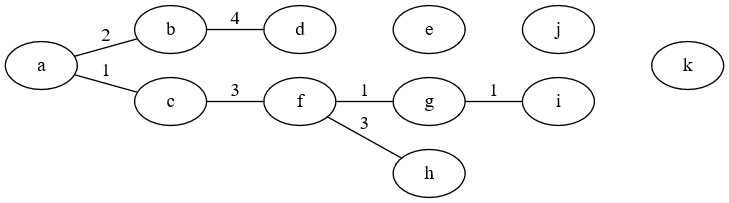
\includegraphics[width=.75\textwidth]{ch-dijkstra/spf8}
  \begin{tabular}{ | c | c | c | c | c | c | c | c | c | c | c | c | }
  \hline
   & $a$ & $b$ & $c$ & $d$ & $e$ & $f$ & $g$ & $h$ & $i$ & $j$ & $k$ \\
   \hline
   distance & 0 & 2 & 1 & 6 & 8 & 4 & 5 & 7 & 6 & $\infty$ & 8 \\
   \hline
   parent & $\emptyset$ & $a$ & $a$ & $b$ & $d$ & $c$ & $f$ & $f$ & $g$ & $\emptyset$ & $i$ \\
   \hline
   relaxed & 1 & 1 & 1 & 1 & 0 & 1 & 1 & 1 & 1 & 0 & 0 \\
   \hline
  \end{tabular}
\caption{Relax $h$. $\delta(a,h) = \delta(a,f) + \delta(f,h) = 4+3=7$}
\label{spf8}
\end{figure}

Relax $e$.

\begin{figure}[H]
\centering
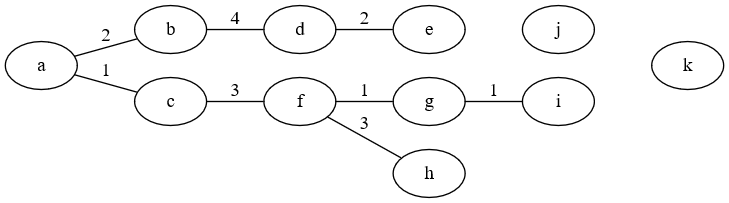
\includegraphics[width=.75\textwidth]{ch-dijkstra/spf9}
  \begin{tabular}{ | c | c | c | c | c | c | c | c | c | c | c | c | }
  \hline
   & $a$ & $b$ & $c$ & $d$ & $e$ & $f$ & $g$ & $h$ & $i$ & $j$ & $k$ \\
   \hline
   distance & 0 & 2 & 1 & 6 & 8 & 4 & 5 & 7 & 6 & 9 & 8 \\
   \hline
   parent & $\emptyset$ & $a$ & $a$ & $b$ & $d$ & $c$ & $f$ & $f$ & $g$ & $e$ & $i$ \\
   \hline
   relaxed & 1 & 1 & 1 & 1 & 1 & 1 & 1 & 1 & 1 & 0 & 0 \\
   \hline
  \end{tabular}
\caption{Relax $e$. $\delta(a,e) = \delta(a,d) + \delta(d,e) = 6 + 2$}
\label{spf9}
\end{figure}

Relax $k$. Notice that this reduces the total distance to $j$ along a longer path.

\begin{figure}[H]
\centering
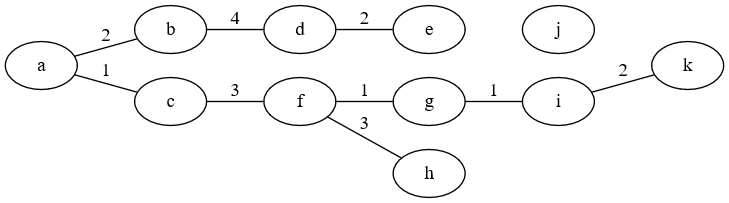
\includegraphics[width=.75\textwidth]{ch-dijkstra/spf10}
  \begin{tabular}{ | c | c | c | c | c | c | c | c | c | c | c | c | }
  \hline
   & $a$ & $b$ & $c$ & $d$ & $e$ & $f$ & $g$ & $h$ & $i$ & $j$ & $k$ \\
   \hline
   distance & 0 & 2 & 1 & 6 & 8 & 4 & 5 & 7 & 6 & 10 & 8 \\
   \hline
   parent & $\emptyset$ & $a$ & $a$ & $b$ & $d$ & $c$ & $f$ & $f$ & $g$ & $k$ & $i$ \\
   \hline
   relaxed & 1 & 1 & 1 & 1 & 1 & 1 & 1 & 1 & 1 & 0 & 1 \\
   \hline
  \end{tabular}
\caption{Relax $k$. $\delta(a,k) = \delta(a,i) + \delta(i,k) = 6 + 8 = 10$}
\label{spf10}
\end{figure}

There is no real reason to relax the final vertex $j$ as it cannot improve the path to any other reached vertex. The shortest path tree is now complete.

\begin{figure}[H]
\centering
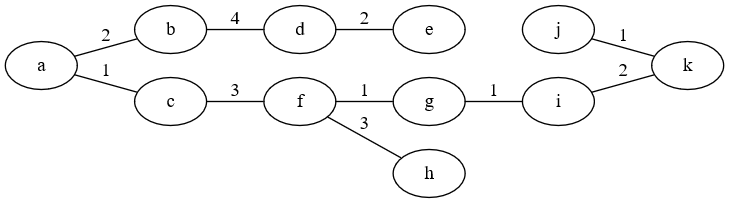
\includegraphics[width=.75\textwidth]{ch-dijkstra/spf11}
\caption{The last vertex $j$ has $\delta(a,j)=\delta(a,k)+\delta(k,j)=9+1=10$}
\label{spf11}
\end{figure}

\chapter{RSA}

\section{Asymmetric Cryptography}
Kerckhoff's principle motivates most modern ciphers: the strength of a cryptosystem should depend only on the secrecy of the keys used, not on the secrecy of the cryptographic algorithm. Some of the most popular algorithms today are Diffie-Hellman, RSA, Elgamal, ECC, 3DES, Rijndael (AES), MD5, and SHA. Each of these algorithms are publicly-known, thoroughly studied, and have been implemented in many programming languages.

Suppose principal $A$ needs to securely pass a message $M$ to another principal $B$. Then $A$ needs some key $k$ that can be used to encrypt the message to ciphertext $C=\texttt{encrypt}(M,k)$. $B$ can reverse the operation with $M=\texttt{decrypt}(C,k)$. How, though, should $A$ and $B$ both obtain the same key $k$?

In many instances it is possible for $A$ and $B$ to use a shared key $k_{ab}$. An example of this might be a Site-to-Site Virtual Private Network (VPN) tunnel. The network administrator must configure each side of the VPN with the same key. If a third principal $C$ is added to the network then it might reuse the same key or be configured with the same key $k_{ab}$ or any combination of new keys $k_{ac}$ and $k_{bc}$.

Reusing keys is not secure and creating $n-1$ keys for each $n$th additional principal is less than optimal. A dynamic and scalable approach is needed. The approach must allow principals with no prior knowledge of one another to encrypt messages with a unique key. \textbf{Asymmetric cryptography} provides precisely this capability.

Each principal in an asymmetric cryptosystem has both a public key $e$ and private key $d$. The public key is used to encrypt a message. The encrypted message can only be decrypted by the corresponding private key. For example, when principal $X$ sends a message $M$ to $A$, $X$ encrypts the message with $A$'s public key $e_a$ to create a ciphertext $C=\texttt{encrypt}(M,e_a)$. Only $A$ possesses the private key $d_a$ to decrypt the original message $M=\texttt{decrypt}(C,d_a)$.

The best-known asymmetric cryptosystem in the world was created by Ronald Linn Rivest, Adi Shamir, and Leonard Max Adelman and published in 1978 \cite{Rivest:1978:MOD:359340.359342}. This algorithm has become known as RSA for the initials of its authors.

The essential characteristic of any asymmetric cryptosystem is that it must contain a \textit{trap-door}. The trap-door property allows an algorithm to work efficiently in its intended use but prohibitively slowly in reverse. The trap-door for RSA is prime factorization.

\section{Large Primes}

The \textit{Prime Number Theorem} states that there exists a unique prime factorization for each integer greater than zero. It is easy to create a composite number by multiplying two primes $p$ and $q$, but factoring the composite $p \times q$ is difficult.

A trivial factorization algorithm of $n=p \times q$ would attempt trial division by 2 and all odd integers 3 to $\sqrt{p \times q}$. This algorithm would complete in at most $1+\frac{\sqrt{n}}{2}$ steps. For large $n$, this calculation is very expensive. Number theorists have discovered sophisticated algorithms for factoring integers more quickly, but these algorithms are still very slow when presented with large $n$.

The second key concept used in RSA is \textit{modular arithmetic}. This concept may be a bit less familiar.

\section{Modular Arithmetic}

Insall and Weisstein define modular arithmetic as a ``the arithmetic of congruences'' \cite{weissteinModular}. The geometric understanding fits nicely. Consider 90\degree and 450\degree angles. These angles may have a different value, but geometrically equal because $90 \equiv 450$.

\subsection{The Modulus Operator}

A numerical understanding of congruence is that it is the remainder after division. The remainder of $\frac{90}{360}$ is 90, as is $\frac{450}{360}$. The \textit{modulus operator} (mod) is a useful function to compute the remainder after division.

\[
90 \equiv 450 \mod 360
\]

Many programming languages use the \texttt{\%} symbol as a modulus operator. Taking any value $\mod 0$ is not allowed as this implies division by zero.

\begin{lstlisting}[caption={The modulus operator in C}, captionpos=b, mathescape, xleftmargin=.25in, xrightmargin=.25in]
#include <stdio.h>

void main () {
  printf("%d\n", (450 % 360)); // prints 90
}

\end{lstlisting}

\subsection{Modular Inverse}

If subtraction is the inverse of addition and division is the inverse of multiplication, then what is the inverse of the modulus operator? This concept is a bit tricky. Typically, we begin with some value $x$ and a modulus $n$ and compute $y \equiv x \mod n$. To go backwards, we find some value $y$ such that $xy \mod n \equiv 1$.

The same modular inverse equation can be written $x x^{-1} \equiv 1 \pmod{n}$ where $y=x^{-1}$. The confusing $-1$ is an unfortunate choice of notation; it is \textbf{not} an exponent.

For example, what is the modular inverse of of $9 \pmod{7}$? That is, what value $y$ satisfies $9y \mod 7 \equiv 1$? Using a simple brute-force approach:

\begin{align*}
(9 \times 1) \mod 7 &\equiv 2 \\
(9 \times 2) \mod 7 &\equiv 4 \\
(9 \times 3) \mod 7 &\equiv 6 \\
(9 \times 4) \mod 7 &\equiv 1
\end{align*}

The modular inverse of 9 (mod 7) is 4. The Euclidean algorithm can be used to calculate a modular inverse efficiently than the brute-force approach shown here \cite{weissteinModular}.

What is the modular inverse of 4 (mod 2)?

\begin{align*}
(4 \times 1) \mod 2 &\equiv 0 \\
(4 \times 2) \mod 2 &\equiv 0 \\
(4 \times 3) \mod 2 &\equiv 0 \\
(4 \times 4) \mod 2 &\equiv 0 \\
\end{align*}

This demonstrates that there exists no $y$ for $xy \mod n \equiv 1$ if $n$ divides $x$. In fact, there exists no $y$ if $n$ and $x$ are not \textit{relatively prime}. Consider the modular inverse of 9 (mod 6).

\begin{align*}
(9 \times 1) \mod 6 &\equiv 3 \\
(9 \times 2) \mod 6 &\equiv 0 \\
(9 \times 3) \mod 6 &\equiv 3 \\
(9 \times 4) \mod 6 &\equiv 0 \\
\end{align*}

9 and 6 have a \textit{greatest common factor} $\textrm{GCF}(9,6)=3$, so they are not relatively prime. There exists no modular inverse of 9 (mod 6).

Proof: If $xy \mod n \equiv 1$ then this implies there exists some integer $k$ such that $xy = kn + 1$ \cite{2101197}.

\[
xy \mod n \equiv 1 \to \exists k \in \mathbb{Z} [xy = kn + 1]
\]

The terms of $xy = kn + 1$ can be rearranged as $1 = xy - kn$. If $x=pq$ and $n=qr$ then $\textrm{GCF}(x,n)=q$ and $1 = pqy - kqr = q (py - kr)$. If $x$ and $n$ are integers then the $1 = q (py - kr)$ only holds when $q = 1$, so $x$ and $n$ must be relatively prime for a modular inverse of $x \pmod{n}$ to exist.

\[
\exists y \in \mathbb{Z} [xy \mod n \equiv 1] \leftrightarrow \textrm{GCF}(x,n)>1 \qed
\]

\section{RSA}

\subsection{Keys Pairs}

RSA key pairs consist of a public key and private key \cite{rfc8017}. The public key is an encryption exponent $e$ and RSA modulus $n$. The private key is a decryption exponent $d$ and the same RSA modulus $n$. $e$, $n$, and $d$ are all positive integers. $n$ is the product of two distinct odd large primes $p$ and $q$.

\subsection{RSA Modulus}
The RSA modulus $n = pq$ is part of the public key, but the values $p$ and $q$ must be kept secret. Recall that the trapdoor for RSA is that multiplication is easy but factorization is difficult. $p$ and $q$ are used to generate $d$, and if an attacker can discover either $p$ or $q$ then recreating $d$ is trivial.

\subsection{RSA Public Exponent}
The value $e$ is most commonly set to 65537. NIST Special Publication 800-78-4 recommends $65537 \le e \le 2^256 - 1$ \cite{Polk2015}. The only steadfast requirement for $e$ is that it must be relatively prime to $(p-1)(q-1)$.

\subsection{RSA Private Exponent}
The value of $d$ is calculated from the the modular inverse of $e \pmod{\phi(p,q)}$, where the Euler Totient Function $\phi(p,q)=(p-1)(q-1)$. \footnote{Version 2.1 of the RSA Cryptography Specification introduced the concept of multi-prime RSA. In multi-prime RSA, $\phi(n)=(p-1)(q-1)$ is replaced with $\lambda(n)=\textrm{LCM}(r_1 - 1, ... , r_u -1)$. LCM is a function to compute the least common multiple. The $r_i$ values are two or more distinct odd primes. \cite{rfc3447}}

\[
ed \equiv 1 \pmod{\phi(p,q)}
\]

\subsection{Encryption and Decryption Primitives}

Euler's totient theorem provides $b^{\phi(m)} \equiv 1 \pmod{m}$ \cite{weissteinModular}. RSA takes advantage of this relatively obscure but well-studied function in its encryption and decryption functions.

\begin{align*}
\texttt{rsa-encrypt}((e,n), M) = C = M^e \mod n \\
\texttt{rsa-decrypt}((d,n), C) = M = C^d \mod n
\end{align*}

These primitives can also be used for digital signatures by using keys in reverse. Let $H=\textrm{hash}(M)$ be the hash of a message $M$. $H$ can be encrypted with the \textbf{private} exponent to create a digital signature $S = H^d \mod n$. Principals with the public key can decrypt the signature $H = S^e \mod n$ and independently recreate $H$.

\chapter{Pointers}

\section{Pointers}

\subsection{Creating a pointer}

Kernighan and Ritchie define ``a pointer is a variable that contains the address of another variable'' \cite{Kernighan:1988:CPL:576122}. In the C programming language, the address of any variable can be found using the \texttt{\&} operator. Variables that contain addresses to other variables (pointers) are declared with a \texttt{*} after their type.

This paper assumes an Intel x86 or x86-64 architecture. Statements related to return addresses and memory corruption will vary in other instruction sets. Additionally, the code presented in this paper has only been tested on Linux using the GNU C Compiler (GCC).

\begin{lstlisting}[caption={Pointers are variables containing memory addresses}, captionpos=b, mathescape, xleftmargin=.25in, xrightmargin=.25in]
#include <stdio.h>
int main()
{
    int x = 5;
    int * y = &x;    
    printf("%d is the value at location %p\n", x, y);
}
\end{lstlisting}
In this example program, an integer \texttt{x} is declared with a value of 5. \texttt{y} is a pointer to \texttt{x}. The location of \texttt{x} will vary each time the program is executed based on where in memory the operating system loads and runs the program. A sample output is \texttt{5 is the value at location 0xa2378614}. 

\subsection{Dereferencing a pointer}

\textit{Dereferencing} a pointer obtains the value at the memory location to which the pointer references. In C, the syntax for this operation is an asterisk (\texttt{*}) before a pointer name. The \texttt{printf} statement in the above program could therefore be rewritten as follows:

\begin{lstlisting}[caption={Pointers are dereferenced with the \texttt{*} operator}, captionpos=b, mathescape, xleftmargin=.25in, xrightmargin=.25in]
    printf("%d is the value at location %p\n", * y, y);
\end{lstlisting}

\texttt{y} is still a pointer to an \texttt{int} variable. This value can be found by dereferencing the pointer with \texttt{* y}.

\subsection{Parameters are passed by value}

Parameters of functions are \textit{passed by value}. This means that the called function receives a copy of the value of the parameter. If the parameter in the called function is modified, the original copy kept by the caller does not change. 

\begin{lstlisting}[caption={Passing the value of a variable to a function}, captionpos=b, mathescape, xleftmargin=.25in, xrightmargin=.25in]
#include <stdio.h>
void increment(int x)
{
  x = x + 1;
}
void main()
{
  int x = 0;
  increment(x);
  printf("%d\n", x); // prints 0
}
\end{lstlisting}

Pointers solve this problem by telling called functions where a variable exists in memory. The called function can then dereference the pointer and manipulate the referenced variable directly.

\begin{lstlisting}[caption={Passing a pointer to a variable to a function}, captionpos=b, mathescape, xleftmargin=.25in, xrightmargin=.25in]
#include <stdio.h>
void increment(int * x)
{
  * x = (* x) + 1;
}
void main()
{
  int x = 0;
  increment(&x);
  printf("%d\n", x); // prints 1
}
\end{lstlisting}

\subsection{Function pointers}

It is also possible to obtain pointers to functions. This is useful for building an abstract, general-purpose program that can use modular components. An example might be a program that accepts a cryptographic function as a parameter. The syntax for declaring functions which accept function pointers looks confusing, but creating a function pointer simply consists of the \texttt{\&} operator before the function name.

\begin{lstlisting}[caption={Function pointers abstract an algorithm from its components}, captionpos=b, mathescape, xleftmargin=.25in, xrightmargin=.25in]
#include <stdio.h>
#include <stdlib.h>

int rsa_encrypt(int m)
{
    // ... example only
    return 1 * m;
}

int elgamal_encrypt(int m)
{
    // ... example only
    return 2 * m;
}

int generic_encrypt(int (* encrypt(int)), int m)
{
    return encrypt(m);
}

void main()
{
    printf("%d\n", generic_encrypt(&rsa_encrypt, 5));     // 5
    printf("%d\n", generic_encrypt(&elgamal_encrypt, 5)); // 10
}
\end{lstlisting}

\section{Arrays}
\subsection{Array syntax is just shorthand for pointer arithmetic}

Arrays in C use square brackets \texttt{[]} as ``syntactical sugar'' to make pointer arithmetic more intuitive. Unlike higher-level languages, arrays are not semantically special in C.

\begin{lstlisting}[caption={Arrays contain consecutive datum of the same type}, captionpos=b, mathescape, xleftmargin=.25in, xrightmargin=.25in]
#include <stdio.h>
void main()
{
    int a[] = { 1, 2, 3 };
    
    int i;
    for (i = 0 ; i < 3 ; i++)
    {
        printf("%d\n", a[i]);    
    }
}
\end{lstlisting}

This program prints each element of the array \texttt{a} on a separate line. The next program uses different syntax to achieve precisely the same result.

\begin{lstlisting}[caption={Square-bracket arrays in C are just pointers}, captionpos=b, mathescape, xleftmargin=.25in, xrightmargin=.25in]
#include <stdio.h>
void main()
{
    int a[] = { 1, 2, 3 };
    int * b = a;
    int i;
    for (i = 0 ; i < 3 ; i++)
    {
        printf("%d\n", * (b + i));
    }
}
\end{lstlisting}

\subsection{Pointer addition}

The statements \texttt{array[position]} and \texttt{* (array + position)} are \textit{roughly} equivalent \cite{lin_pointer_2003}. Roughly, because the compiler handles an additional detail that becomes obvious when the addresses are shown. Expand the \texttt{printf} statement with the following:

\begin{lstlisting}[caption={todo}, captionpos=b, mathescape, xleftmargin=.25in, xrightmargin=.25in]
        printf("%d at %p\n", * (b + i), b + i);
\end{lstlisting}

Output will vary, but it will resemble

\begin{lstlisting}[caption={todo}, captionpos=b, mathescape, xleftmargin=.25in, xrightmargin=.25in]
1 at 0x34cbb820                          
2 at 0x34cbb824                          
3 at 0x34cbb828
\end{lstlisting}

The addresses differ by 4 bytes, not 1. This is because the size of an \texttt{int} is 4 bytes...on this computer. An unfortunate source of complexity with the C programming language is that the various data types may have different sizes on different platforms. In cases where a programmer needs a variable of a specific width, the \texttt{stdint.h} header provides fixed-width types, such as \texttt{uint32\_t} (unsigned, 32-bit integer type). Otherwise, programmers can use the \texttt{sizeof} operator to find the size of a value at compile-time.

The compiler will implicitly multiply any value added to a pointer by the size of the type. In other words, \texttt{a[i] = * (a + i * sizeof(type)}.

\subsection{Obfuscated C}

The following program compiles and runs with no errors:

\begin{lstlisting}[caption={todo}, captionpos=b, mathescape, xleftmargin=.25in, xrightmargin=.25in]
#include <stdio.h>
void main()
{
    int a[2] = { 1234, 5678 };
    printf("%d\n", 0[a]); // 1234
    printf("%d\n", 1[a]); // 5678
}
\end{lstlisting}

The compiler sees the integers 0 and 1, multiplies them by \texttt{sizeof(int)}, and adds this product to \texttt{* a} to find the memory locations \texttt{0[a]} and \texttt{1[a]}. Syntactical tricks like this are not recommended in production...

\section{Memory operations}

\subsection{The \texttt{sizeof} operator}

\begin{lstlisting}[caption={todo}, captionpos=b, mathescape, xleftmargin=.25in, xrightmargin=.25in]
#include <stdio.h>
#include <stdint.h>
void main()
{
    printf("%d\n", sizeof(int));       // 4
    printf("%d\n", sizeof(uint16_t));  // 2
}
\end{lstlisting}

The \texttt{sizeof} operator computes the size of a data structure in C.

\subsection{The \texttt{malloc}, \texttt{calloc}, and \texttt{free} operators}

The \texttt{sizeof} operator is very useful when manually allocating memory with the \texttt{malloc} and \texttt{calloc} function. \texttt{malloc} allocates the requested number of bytes and returns a pointer to the first one. \texttt{calloc} does the same and also places the value \texttt{0x00} in each byte. Programs that invoke \texttt{malloc} and \texttt{calloc} must use the \texttt{free} function to relinquish memory allocated back to the operating system. All of these functions are provided by the \texttt{stdlib.h} header.

\begin{lstlisting}[caption={todo}, captionpos=b, mathescape, xleftmargin=.25in, xrightmargin=.25in]
#include <stdio.h>
#include <stdlib.h>
#define N 4
void main()
{
    int * x = malloc(sizeof(int) * N);
    int i = 0;
    while (i < N)
    {
        * (x + i) = i;
        printf("%d\n", * (x + i));
        i++;
    }
    free(x);
}
\end{lstlisting}

The above program demonstrates the use of \texttt{malloc} and \texttt{free}. A loop both assigns and prints values $[0,n)$ into the array represented by \texttt{x}. This program uses the \texttt{\#define} preprocessor directive to replace all instances of ``\texttt{N}'' with the string ``\texttt{4}''. A general-purpose solution might be to accept the number of integers as a command-line parameter. In this case, the \texttt{atoi} function in \texttt{stdlib.h} can be useful.

\begin{lstlisting}[caption={todo}, captionpos=b, mathescape, xleftmargin=.25in, xrightmargin=.25in]
#include <stdio.h>
#include <stdlib.h>
void main(int argc, char ** argv)
{
    int n = (argc > 1) ? atoi(argv[1]) : 4;
    int * x = malloc(sizeof(int) * n);
    int i = 0;
    while (i < n)
    {
        * (x + i) = i;
        printf("%d\n", * (x + i));
        i++;
    }
    free(x);
}
\end{lstlisting}

\subsection{Character arrays}

Unlike previous code examples, the above program accepts \textit{command-line arguments}. These are the parameters typed after the name of a program invoked at a command prompt. In C, the value \texttt{argv[0]} is always populated with the name of the command executed and therefore \texttt{argc} will always be greater than zero. Parameters entered after the name of the program are represented as character arrays in positions \texttt{argv[1]}, \texttt{argv[2]}, etc. Remember that arrays in C are effectively interchangeable with pointers. This program uses the syntax \texttt{char ** argv} but the form \texttt{char * argv[]} will also compile and may produce identical machine code.

Just as C hardly gives special treatment to arrays, C barely acknowledges any uniqueness for strings. Strings are simply arrays of characters and are terminated by a \texttt{char} with the value \texttt{0x00}. This ``null'' character can be represented in C as \texttt{'\char`\\0'} (including the single quotes). So, the string ``hello'' in ASCII characters should be represented as an array of the form \texttt{char hello[] = \{ 'h', 'e', 'l', 'l', 'o', '\char`\\0' \}}.

Why the ``null'' terminator? Remember, C arrays are just pointers. Unlike arrays in high-level languages like Java, \textbf{the C array has no mechanism to track its own length}.

\subsection{Linked Lists}
A \textit{linked list} is a data structure that contains values and a pointer to the next element in the data structure. This program reads four integers into a linked list data structure, then destroys the data structure using \texttt{free} as the program closes.

\begin{lstlisting}[caption={A quick and simple linked list}, captionpos=b, mathescape, xleftmargin=.25in, xrightmargin=.25in]
#include <stdio.h>
#include <stdlib.h>
#define N 4

typedef struct _l {
    int v;
    struct _l * n;
} link;

void main()
{
    int x = 0;
    link * first;
    link * current;
    
    for (x = 0; x < N; x++) {
        if (current == NULL)
            first = current = malloc(sizeof(link));
        else
            current = current->n = malloc(sizeof(link));
        printf("Enter integer: ");
        scanf("%d", &current->v);
    }
    
    for (x = 0, current = first; x < N; x++) {
        printf("%d\n", current->v);
        link * last = current;
        current = current->n;
        free(last);
    }
}
\end{lstlisting}

\subsection{Illegal access}

This program also reads input command prompt using the \texttt{scanf} function, but it contains a bug.

\begin{lstlisting}[caption={todo}, captionpos=b, mathescape, xleftmargin=.25in, xrightmargin=.25in]
#include <stdio.h>
#include <stdlib.h>
void main(int argc, char * argv[])
{
    int n = (argc > 1) ? atoi(argv[1]) : 4;
    int * x = malloc(sizeof(int) * n);
    int i = 0;
    while (i <= n)
    {
        printf("%p = ", x + i);
        scanf("%d", x + i);
        printf("%d\n", * (x + i));
        i++;
    }
    free(x);
}
\end{lstlisting}

An example output is shown below, invoking the program without a command-line argument and thus leaving \texttt{n} at the default value of four.

\begin{lstlisting}[caption={todo}, captionpos=b, mathescape, xleftmargin=.25in, xrightmargin=.25in]
0x614010 = 5                           
5      
0x614014 = 3                           
3
0x614018 = 7                           
7
0x61401c = 12                           
12
0x614020 = 888
888
\end{lstlisting}

Look closely and notice that this output had \textbf{five} lines of output, not four. Why did this change? This bug was introduced by looping on \texttt{i <= n} instead of \texttt{i < n}.

This subtle bug reveals some unexpected aspects of programming with C. First, a program can compute a pointer to a memory location that has not been allocated by the operating system. Second, it may or may not be possible to read and write to this location in memory, and the operating system might not produce any errors. In this case, the operating system allocated sixteen bytes for \texttt{x} but produced no warning when the program wrote 888 outside of this range.

Again, recall that the C array has no builtin mechanism to manage its own length. In fact, these simple, pointer-based arrays have no means to expand and contract, search, sort, or otherwise manage the data. An array is just a pointer to the head element -- nothing more. C++ has a more sophisticated \texttt{std::vector} class. Many commercial and open-source data structures are available to provide more features than the basic C array.

\section{Pointer errors}

\subsection{Incorrect \texttt{free} operations}
The previous program got away with an illegal write. It is also very common for programs to crash with the vague and dreaded message \texttt{Segmentation fault}.

\begin{lstlisting}[caption={todo}, captionpos=b, mathescape, xleftmargin=.25in, xrightmargin=.25in]
#include <stdio.h>
#include <stdlib.h>
void main(int argc, char * argv[])
{
    int a[] = { 0 , 1 };
    free(a);
}
\end{lstlisting}

This benign-looking program attempts to \texttt{free} memory that has been allocated on the \textit{stack} and crashes.

Many C compilers allocate memory for arrays and ordinary variables in an area shared by the instructions of the program executed. As functions call other functions, the state at each layer is preserved in a data structure described as a \textit{stack}. It is neither legal nor necessary to \texttt{free} the instructions and variables declared along the stack.

\texttt{malloc} and \texttt{calloc} allow programmers to obtain memory in a different area called the \textit{heap}. Variables on the heap can be shared among functions at any layer of the stack through pointers.

A similar example leads somehow to a slightly different result:

\begin{lstlisting}[caption={todo}, captionpos=b, mathescape, xleftmargin=.25in, xrightmargin=.25in]
#include <stdio.h>
#include <stdlib.h>
void main(int argc, char * argv[])
{
    free(argv);
}
\end{lstlisting}

Strangely, attempting to free clearly illegal memory ranges works fine:

\begin{lstlisting}[caption={todo}, captionpos=b, mathescape, xleftmargin=.25in, xrightmargin=.25in]
#include <stdio.h>
#include <stdlib.h>
int main(int argc, char * argv[])
{
    free(0x00000000);
    printf("No segfaults here.\n"); // prints without error
}
\end{lstlisting}

Is a memory location still accessible after calling \texttt{free}?

\begin{lstlisting}[caption={todo}, captionpos=b, mathescape, xleftmargin=.25in, xrightmargin=.25in]
#include <stdio.h>
#include <stdlib.h>
int main(int argc, char * argv[])
{
    int * x = calloc(sizeof(int), 1);
    * x = 1234;
    printf("%d\n", * x); // 1234
    free(x);
    printf("%d\n", * x); // 0
}
\end{lstlisting}

The memory location is emptied but still writable. 

\begin{lstlisting}[caption={todo}, captionpos=b, mathescape, xleftmargin=.25in, xrightmargin=.25in]
#include <stdio.h>
#include <stdlib.h>
int main(int argc, char * argv[])
{
    int * x = calloc(sizeof(int), 1);
    * x = 1234;
    printf("%d\n", * x); // 1234
    free(x);
    * x = 4321;
    printf("%d\n", * x); // 4321
}
\end{lstlisting}

\subsection{Illegal accesses}

The following program allocates a valid pointer but writes to the heap beyond this pointer. How long can this persist? The program will segfault after many successful writes.

\begin{lstlisting}[caption={todo}, captionpos=b, mathescape, xleftmargin=.25in, xrightmargin=.25in]
#include <stdio.h>
#include <stdlib.h>
void main()
{
    int * x = malloc(sizeof(int));
    while (1)
    {
        * x = 4;
        printf("%p\n", x);
        x++;
    }
}
\end{lstlisting}

And on the stack? The crash is almost immediate.

\begin{lstlisting}[caption={todo}, captionpos=b, mathescape, xleftmargin=.25in, xrightmargin=.25in]
#include <stdio.h>
#include <stdlib.h>
void main()
{
    int y = 0;
    int * x = &y;
    while (1)
    {
        * x = 4;
        printf("%p\n", x);
        x++;
    }
}
\end{lstlisting}

Errors and crashes are the expected result from writing to invalid memory locations. These programs wrote to memory locations on the stack near where local variables are represented. The next program explores this area of memory a more closely.

\subsection{Memory on the stack}

\begin{lstlisting}[caption={todo}, captionpos=b, mathescape, xleftmargin=.25in, xrightmargin=.25in]
#include <stdio.h>

void find()
{
    long offset = -3;
    printf("offset is at %p\n", &offset);
    while (offset <= 3)
    {
        printf("[%2d] Location %p has value %p\n", offset,
            &offset + offset, * (&offset + offset));
        offset++;
    }
}

void main()
{
    int x = 0;
    printf("main() is at %p\n", &main);
    printf("find() is at %p\n", &find);
    printf("integer x at %p\n", &x);
    find();
}
\end{lstlisting}

This program shows what exists in memory near a variable named \texttt{offset}. The program also makes use of function pointers to find where on the stack \texttt{main} and \texttt{find} are located.

\begin{lstlisting}[caption={todo}, captionpos=b, mathescape, xleftmargin=.25in, xrightmargin=.25in]
main() is at 0x400780          
find() is at 0x400900    
integer x at 0x7ffe8e1444b4    
offset is at 0x7ffe8e144490
[-3] Location 0x7ffe8e144478 has value (nil)
[-2] Location 0x7ffe8e144480 has value 0x400800
[-1] Location 0x7ffe8e144488 has value 0x400958
[ 0] Location 0x7ffe8e144490 has value (nil)
[ 1] Location 0x7ffe8e144498 has value 0xf2f82083df84b100
[ 2] Location 0x7ffe8e1444a0 has value 0x400800
[ 3] Location 0x7ffe8e1444a8 has value 0x4007e3
\end{lstlisting}

Notice that the memory locations near \texttt{offset} contain values between \texttt{0x400700} and \texttt{0x400a00}. Pointers to the \texttt{main} and \texttt{find} functions happen to be in the same range. This is not a coincidence.

Discovery-based learning at this stage becomes very difficult. Reverse-engineering a compiled C program from memory dumps requires a great deal of foundational knowledge that is not easily achieved. The value \texttt{0x4007e3} is a magic value -- it is the return address.

The stack maintains a pointer to the caller of a function. The compiled assembly language will ``jump'' back to the caller once a function completes. The GNU C Compiler offers a special instruction named \texttt{\_\_builtin\_return\_address} to expose this value to programs.

\begin{lstlisting}[caption={todo}, captionpos=b, mathescape, xleftmargin=.25in, xrightmargin=.25in]
void find()
{
    long offset = -3;
    printf("offset is at %p\n", &offset);
    while (offset <= 3)
    {
        printf("[%2d] Location %p has value %p\n", offset,
            &offset + offset, * (&offset + offset));
        offset++;
    }
    printf("Return address is %p\n", __builtin_return_address(0));
}
\end{lstlisting}

Adding this statement produces the expected output ``\texttt{Return address is 0x4007e3}.''

\subsection{Controlling the jump}

It is possible for a C program to modify the return pointer that restores program control to the callers of functions.

\begin{lstlisting}[caption={todo}, captionpos=b, mathescape, xleftmargin=.25in, xrightmargin=.25in]
#include <stdio.h>
void test()
{
    long * r = &r + 3;
    printf("Return address is %p\n", * r);
    * r = &test;
}
void main()
{
    test();
}
\end{lstlisting}

This program creates a pointer \texttt{* r} to the return address that is expected to exist at location \texttt{\&r + 3}. It prints this value and then overwrites its contents with \texttt{\&test}, a pointer to the \texttt{test} function. When the \texttt{test} function completes, the computer ``jumps'' to the beginning of \texttt{test} and executes the function a second time. On the second execution the pointer \texttt{* r} refers to a different location and writes to it anyways. The cycle continues until the program attempts to write to a location in memory that causes a crash.

\begin{lstlisting}[caption={todo}, captionpos=b, mathescape, xleftmargin=.25in, xrightmargin=.25in]
Return address is 0x7f130dfa5ec5         
Return address is (nil)
Return address is 0x7ffd51a559a8     
Return address is 0x100000000   
Return address is 0x400780     
Return address is (nil)
Return address is 0xdc5fe1af2040fe1a
Return address is 0x4007e0
Return address is 0x7ffd51a559a0
...
Return address is 0x6f6f723d52455355
Return address is 0x682f3d4457500074
Return address is 0x6d6f682f00656d6f
Return address is 0x74756f2e612f65     
Return address is (nil)             
Segmentation fault
\end{lstlisting}

Effectively exploiting memory corruption is difficult and error-prone.

\subsection{Stack smashing}

The following program looks completely benign. It accepts two integers as input from the console and prints their product.

\begin{lstlisting}[caption={todo}, captionpos=b, mathescape, xleftmargin=.25in, xrightmargin=.25in]
#include <stdio.h>
void main()
{
    int x, y;
    
    printf("x = ");
    scanf("%ld", &x);
    
    printf("y = ");
    scanf("%ld", &y);
    
    printf("x * y = %ld\n", x * y);
}
\end{lstlisting}

The program compiles, runs, and even works for obvious inputs. However, this program contains a very serious bug.

\begin{lstlisting}[caption={todo}, captionpos=b, mathescape, xleftmargin=.25in, xrightmargin=.25in]
x = 0
x = 8589934588
x * y = 4294967292
\end{lstlisting}

The above output may be difficult to reproduce. First, modern compilers and integrated development environments (such as Visual Studio) aggressively discourage the use of \texttt{scanf} for its well-known security flaws. Second, compilers should show warnings or even errors on the ``\texttt{\%ld}.'' This scanning pattern is incorrect. It reads the input as a \textit{long} decimal integer, but \texttt{x} and \texttt{y} are not declared \texttt{long}. As a result, it is possible for bytes of \texttt{y} to overflow into \texttt{x}.

If using GCC, it may be necessary to compile this program with the option \texttt{-fno-stack-protector}. With stack protection enabled the program may crash with the error \texttt{*** stack smashing detected ***: /home/a.out terminated}.

\subsection{Jumping from user input}
The next program is a bit contrived. It takes user input and stores it the location of the return pointer.

\begin{lstlisting}[caption={todo}, captionpos=b, mathescape, xleftmargin=.25in, xrightmargin=.25in]
#include <stdio.h>
void hello() {
    printf("Hello world!\n");
}

void world() {
    long i = &i + 3;
    printf("Enter %p and see what happens: ", &hello);
    scanf("%x", i);
}

int main()
{
    world();
    printf("Completed");
    return 0;
}
\end{lstlisting}

The program never invokes \texttt{hello()}, but the user can.

\begin{lstlisting}[caption={todo}, captionpos=b, mathescape, xleftmargin=.25in, xrightmargin=.25in]
Enter 0x400920 and see what happens: 0x400920       
Hello world!
Segmentation fault
\end{lstlisting}

\subsection{A less-contrived jump from user input}

The next program contains a bug that is intended to be slightly more plausible. The approach to obtaining user input is not entirely far-fetched.

\begin{lstlisting}[caption={todo}, captionpos=b, mathescape, xleftmargin=.25in, xrightmargin=.25in]
#include <stdio.h>

void hello()
{
    printf("Hello world!\n");
}

long * read()
{
    long values[4];
    int i = 0;
    int last = 0;
    printf("Enter a list of values. Enter -1 to stop.\n");
    while (last != -1)
    {
        scanf("%lx", &values[i]);
        last = values[i];
        i++;
    }
    return values;
}

int main()
{
    printf("hello() is located at %p\n", &hello);
    read();
    return 0;
}
\end{lstlisting}

Admittedly, no program in production would expose the memory location of a function like this, but it is simple for an attacker to reverse engineer the inner workings of a C program with tools such as the GNU Debugger (GDB). This program reveals \texttt{\&hello} for pedagogical convenience.

\begin{lstlisting}[caption={todo}, captionpos=b, mathescape, xleftmargin=.25in, xrightmargin=.25in]
hello() is located at 0x4005ed
Enter a list of values. Enter -1 to stop.
0x4005ed
0x4005ed
0x4005ed
0x4005ed
0x4005ed
0x4005ed
0x4005ed
-1
Hello world!
Hello world!
Segmentation fault (core dumped)
\end{lstlisting}

The program executes the \texttt{hello} function (twice) and crashes based only on user input. The \texttt{read} function contains several flaws. First, the method returns a non-static local array named \texttt{values}. Recall that these variables are declared on the stack, not the heap, and will be automatically created and destroyed as the program executes. This program would not have worked as intended, and GCC produces a warning ``\texttt{function returns address of local variable}.''

The second flaw in \texttt{read} is that it uses an unusual halting condition: the input of \texttt{-1}. It would have been a better choice to halt on more standard mechanisms such as Ctrl + D. This function was intentionally written poorly, but unfortunately it is not unusual for strange decisions like this to be found in production code. Protocols old and new may interpret ordinary input in special ways.

Finally, the problematic halting condition allows a disastrous buffer overflow attack because the algorithm does not check if \texttt{i} is greater than the length of \texttt{values}.

\section{Defending against buffer overflow attacks}

\subsection{Bugs}
The class of bugs where user input is allowed to exceed the size of a buffer and overwrite return pointers is known as \textit{buffer overflow attacks} \cite{Erickson:2008:HAE:1407147}.

Linus Torvalds famously maintains that ``security problems are just bugs'' \cite{torvalds_2017}. From this perspective, the buffer overflow is a flaw in the correctness of a program. An input to an algorithm can lead to behavior not intended by the implementor.

A buffer overflow, which may lead to arbitrary code execution, is an extreme result of a program that does not correctly handle input. All serious programming efforts should include extensive testing. For suitably small inputs it may be reasonable to attempt all possible values or all possible combinations.

For example, consider a function $f(x)$ that accepts a single unsigned byte $x$ as an input. Suppose the software specification defines only three valid values for $x$: 0, 1, and 3. A single byte can hold only 256 possible values, so it would be prudent to test all possible values $0 \le x < 256$.

Suppose that a related function $g(x)$ accepts an array of bytes $x$ as an input. $x$ should have a well-defined minimum and maximum length. The behavior of $g(x)$ should be well-defined if $x$ is null or inaccessible. If the maximum length of $x$ is very short then it is possible to test all possible values $x$, but as the length of $x$ increases then the number of possible inputs grows exponentially. So larger inputs, testers can ``fuzz'' $g(x)$ using a program to generate sequential, random, or malformed data. Fuzzing is a technique for black-box testing.

Black-box testing can be used in parallel to white-box testing. White-box tests may include code reviews by other programmers, source code analysis with bug detection programs, and formal verification.

Theoretically, formal verification is the most effective solution of proving that a computer program correctly implements an algorithm \cite{hartnett_quanta}. Unfortunately, formal methods are far beyond the skill level of typical programmers.

\subsection{Languages}
Java, JavaScript, C\#, Python, PHP, and Visual Basic are among the most popular programming languages in the world. None of these languages support pointer arithmetic. It is possible to create a variable that contains a memory address, but these variables are called \textit{references}. References can be passed as parameters to functions with the same semantics as C passing a pointer as an argument.

Pointers in C and C++ can be very useful for low-level and high-performance programming. Device drivers and networking protocols can benefit from direct access to memory. Game developers and other authors of performance-sensitive software often seek to take advantage of memory tricks to optimize algorithms for speed. Direct accesses to memory may come with risks to maintainability, portability, correctness, and security.

Recall that arrays in C are simply pointers. This technique is fast and efficient but it does nothing to prevent programmers to reading and writing to invalid locations. Many languages have more robust arrays that cannot be as easily exploited.

\subsection{Operating systems}
Modern operating systems provide many features that can mitigate the impact of buffer overflow attacks in buggy code.

The most common form of buffer overflow attack is to overwrite the return address in the stack frame \cite{apple}. An obvious protection that the operating system or intrusion prevention software can take is to detect and prevent unexpected writes to the stack frame.

A second enhancement that modern operating systems provide is address space layout randomization (ASLR). As the name implies, ASLR makes memory corruption attacks more difficult by randomizing the location where the stack, heap, and libraries might be located.

Modern processors allow operating systems to mark portions of memory non-executable \cite{apple}. Finally, modern compilers have several features (such as \texttt{-fstack-protector}) that insert runtime checks for memory corruption.

\subsection{Unsafe library functions}
Many legacy functions in C standard libraries are known to be unsafe. These unsafe functions include \texttt{strcpy}, \texttt{scanf}, and dozens more.

\chapter{Binary}

\section{Positional Number Systems}
In the \textit{Hindu-Arabic Number System}, numbers are expressed as strings of digits \cite{ji_2010}. They are read left-to-right, where each digit multiplies a descending power of the \textit{base} or \textit{radix}. The string of digits ``10'' denotes the smallest integer greater than the largest allowable digit. Decimal (base 10) was introduced to the west largely by Leonardo Pisano Bogollo, better known as ``Fibonacci'' \cite{seligman_2011} \cite{mastin_2010}.

The value ``2017'' in decimal is equal to $2 \times 10^3 + 0 \times 10^2 + 1 \times 10^1 + 7 \times 10^0$. A concept of zero is essential in order to skip empty positions. An alternative number system is Roman Numerals \cite{ji_2010}.

Binary is simply a positional number system with only two digits, 0 and 1. The value $0\texttt{b}10100110 = 1 \times 0\texttt{b}10^7 + 0 \times 0\texttt{b}10^6 + 1 \times 0\texttt{b}10^5 + 0 \times 0\texttt{b}10^4 + 0 \times 0\texttt{b}10^3 + 1 \times 0\texttt{b}10^2 + 1 \times 0\texttt{b}10^1 + 0 \times 0\texttt{b}10^0$ where the radix ``10'' is equal to decimal 2. The prefix $0\texttt{b}$ is used to distinguish binary literals from decimal numbers in several languages, including C, C++, C\#, Java, and JavaScript \cite{oracle_binary_literal}.

\section{Signed Binary Numbers}\label{signedbinary}

\subsection{Signed Magnitude}

Mathematical notation for signed numbers uses the ``$-$'' symbol to mark a number negative. This approach can be used in computers by reserving the leftmost bit in a string of bits to denote sign, where 0 is positive and 1 is negative. This notation is simple to understand, but it is not commonly used because it is slower and more complex to implement in hardware than one's complement and two's complement \cite{smoler}.

\subsection{One's Complement}
In one's complement the high-order bit indicates sign. If this bit is 1 then the remaining bits are inverted \cite{lin_onescomp_2003}. Thus, the value $0\texttt{b}1010$ is equal to -5.

One's complement is very simple to compute: simply invert all the bits to negate a value. This strategy leads to some interesting results. For example, there are two zeros in one's complement ($0\texttt{b}0000$ and $0\texttt{b}1111$). Addition to a value and its one's complement cause an overflow. If the overflowing bit is ignored then the result is correct.

\begin{equation*}
\begin{array}{c}
\phantom{+}0\texttt{b}0100 \phantom{+}(+4) \\
\underline{+0\texttt{b}1011 \phantom{+}(-4)} \\
0\texttt{b}0000 \phantom{+}(0)
\end{array}
\end{equation*}

The range for a one's complement value of $n$ bits is $[-(2^{n-1}-1),2^{n-1}-1]$. If the sum of two values $a$ and $b$ is greater than $2^{n-1}-1$ then the result will overflow and become negative. Integer overflow is very common when programming with typed values of finite size \cite{seacord_2017}.

Addition of one's complement does not work very well. Take, for example, $-0 + 1$. The high-ordered one overflows. When truncated, the value is equal to $-0$.

\begin{equation*}
\begin{array}{c}
\phantom{+}0\texttt{b}1111 \phantom{+}(-0) \\
\underline{+0\texttt{b}0001 \phantom{+}(+1)} \\
\phantom{+}0\texttt{b}1111 \phantom{+}(-0)
\end{array}
\end{equation*}

In fact, adding any $a > 0$ and $b < 0$ where $a \ne -b$ causes problems.

\begin{equation*}
\begin{array}{c}
\phantom{+}0\texttt{b}0101 \phantom{+}(+5) \\
\underline{+0\texttt{b}1011 \phantom{+}(-4)} \\
\phantom{+}0\texttt{b}0000 \phantom{+}(+0)
\end{array}
\end{equation*}

The result is off by one.

\subsection{Two's Complement}

Two's complement is another method for representing integers in binary. Two's complement allows addition and subtraction of positive and negative integers to work correctly \cite{finley_2000}.

To convert a positive value to a negative value, invert all the bits \textit{and add one}. Sounds strange but it works. If $113 = 0\texttt{b}01110001$ then $-113 = 0\texttt{b}10001110 + 1 = 0\texttt{b}10001111$. We demonstrate that two's complement works for $a - a = 0$ where $a = 113$:

\begin{equation*}
\begin{array}{c}
\phantom{+}0\texttt{b}01110001 \phantom{+}(+113) \\
\underline{+0\texttt{b}10001111 \phantom{+}(-113)} \\
\phantom{+}0\texttt{b}00000000 \phantom{+}(+0)\phantom{9}\phantom{9}
\end{array}
\end{equation*}

Now we demonstrate $b - a > 0$ where $a = 113$ and $b = 120 = 0\texttt{b}01111000$ in two's complement:

\begin{equation*}
\begin{array}{c}
\phantom{+}0\texttt{b}01111000 \phantom{+}(+120) \\
\underline{+0\texttt{b}10001111 \phantom{+}(-113)} \\
\phantom{+}0\texttt{b}00000111 \phantom{+}(+7)\phantom{9}\phantom{9}
\end{array}
\end{equation*}

Finally $b - a < 0$ where $a = 120 = 0\texttt{b}01111000$ and $b = 113$. $-120 = 0\texttt{b}10000111 + 1 = 0\texttt{b}10001000$.

\begin{equation*}
\begin{array}{c}
\phantom{+}0\texttt{b}01110001 \phantom{+}(+113) \\
\underline{+0\texttt{b}10001000 \phantom{+}(-120)} \\
\phantom{+}0\texttt{b}11111001 \phantom{+}(-7)\phantom{9}\phantom{9}
\end{array}
\end{equation*}

Converting back to decimal, $0\texttt{b}11111001 \textrm{ (two's complement)} = 0\texttt{b}11111001 \textrm{ (one's complement)} - 1 = -0\texttt{b}00000111 = -(2^2 + 2^1 + 2^0) = -7$. This is consistent with our expectations.

\section{Bit Operations}

Computers handle bits using the same rules as Boolean Logic. Let $1=T$ ($T$ means ``true'') and $0=F$ ($F$ means ``false'') and well-established rules of discrete mathematics. An important distinction between bit operations and Boolean algebra is that computers usually operate on many bits at once.

\subsection{And}

The ``and'' operation is represented by $\wedge$ in mathematics and \texttt{\&} in many programming languages. A \textit{truth table} is a useful tool for showing all possible (discrete) outcomes of Boolean operations. A truth table of the ``and'' operation is shown below.

\begin{equation*}
\begin{array}{c|c|c}
p & q & p \wedge q \\
\hline
T & T & T \\
T & F & F \\
F & T & F \\
F & F & F
\end{array}
\end{equation*}

Equivalently in binary,

\begin{equation*}
\begin{array}{c|c|c}
\texttt{p} & \texttt{q} & \texttt{p\&q} \\
\hline
1 & 1 & 1 \\
1 & 0 & 0 \\
0 & 1 & 0 \\
0 & 0 & 0
\end{array}
\end{equation*}

When computers perform the \texttt{\&} operation on \textit{words} consisting of more than one bit, the individual bits of each word are ``anded'' against those in the corresponding position in the other word. Assume that the following binary strings of digits are unsigned.

\begin{equation*}
\begin{array}{c}
\phantom{\texttt{\&}}0\texttt{b}10110001 \phantom{+}(177) \\
\underline{\texttt{\&}0\texttt{b}11110000 \phantom{+}(240)} \\
\phantom{\texttt{\&}}0\texttt{b}10110000 \phantom{+}(176)
\end{array}
\end{equation*}

This is the logic by which \textit{subnet masks} are used in Internet Protocol (IP) version 4 to separate host addresses from routes. IP addresses are simply unsigned 32-bit integers. A \textit{subnet mask} is used to indicate the bits that are significant for routing an IP packet across the network. The remaining bits are used to address a unique host on that network \cite{rfc791}.

\begin{equation*}
\begin{array}{c}
\phantom{\texttt{\&}}0\texttt{b}11000000\_10101000\_10000001\_00000110 \phantom{.}(192.168.129.6) \\
\underline{\texttt{\&}0\texttt{b}11111111\_11111111\_11111110\_00000000 \phantom{.}(255.255.254.0)} \\
\phantom{\texttt{\&}}0\texttt{b}11000000\_10101000\_10000000\_00000000 \phantom{.}(192.168.128.0)
\end{array}
\end{equation*}

The \texttt{\&} operator shown is considered a \textit{bitwise} operation used to compute values based on inputs. Many programming languages would compute \texttt{x \& y \& z} from left to right. Occasionally it can be useful to evaluate the second and beyond arguments conditionally based on left arguments. In the case of $x \wedge y \wedge z$, if $x = F$ then the values of $y$ and $z$ do not matter -- the result will always be $F$. The \textit{conditional-and operator} is an example of \textit{short-circuit} logic and is represented as a doubled \texttt{\&\&} operator in many programming languages, such as Java \cite{Gosling:2014:JLS:2636997}.

\subsection{Or}

The ``or'' operation is similar in syntax and semantics to the ``and'' operation. The mathematical symbol for ``or'' is $\vee$ and many programming languages use the pipe character, \texttt{|}.

\begin{multicols}{2}

\begin{equation*}
\begin{array}{c|c|c}
p & q & p \vee q \\
\hline
T & T & T \\
T & F & T \\
F & T & T \\
F & F & F
\end{array}
\end{equation*}

\begin{equation*}
\begin{array}{c|c|c}
\texttt{p} & \texttt{q} & \texttt{p|q} \\
\hline
1 & 1 & 1 \\
1 & 0 & 1 \\
0 & 1 & 1 \\
0 & 0 & 0
\end{array}
\end{equation*}

\end{multicols}

The English word ``or'' is implicitly an \textit{inclusive or}, where $T \vee T \equiv T$. \textit{Exclusive or} ($\oplus$), by contrast, satisfies the statement

\begin{equation*}
p \oplus q \equiv \neg (p \wedge q) \wedge (p\vee q)
\end{equation*}

$\neg$ (``not'') inverts the output of $p \wedge q$. ``XOR'' is a common contracted form for the term ``exclusive or.'' Exclusive or is represented by $\oplus$ in math and \textasciicircum in many programming languages.

\begin{multicols}{2}

\begin{equation*}
\begin{array}{c|c|c}
p & q & p \oplus q \\
\hline
T & T & F \\
T & F & T \\
F & T & T \\
F & F & F
\end{array}
\end{equation*}

\begin{equation*}
\begin{array}{c|c|c}
\texttt{p} & \texttt{q} & \texttt{p\textasciicircum q} \\
\hline
1 & 1 & 0 \\
1 & 0 & 1 \\
0 & 1 & 1 \\
0 & 0 & 0
\end{array}
\end{equation*}

\end{multicols}

\subsection{Not}

The $\neg$ operator is represented in many programming languages by an exclamation point, \texttt{!}. $\wedge$, $\vee$, and $\oplus$ are all \textit{binary operators} that accept two parameters. $\neg$ is a \textit{unary operator} that accepts only a single parameter.

\begin{multicols}{2}

\begin{equation*}
\begin{array}{c|c}
p & \neg p \\
\hline
T & F \\
F & T
\end{array}
\end{equation*}

\begin{equation*}
\begin{array}{c|c}
\texttt{p} & \texttt{!p} \\
\hline
1 & 0 \\
0 & 1
\end{array}
\end{equation*}

\end{multicols}

The \texttt{!} operation can be used to compute the broadcast address in an IPv4 subnet. Per RFC919, the address of every subnet with all host bits set is used as a subnet local broadcast \cite{rfc919}.

\subsection{Bit Shift}

Many languages offer a \textit{bit shift} operator that moves bits to the left or right, discarding overflowing bits and replacing them at the opposite end with zeros \cite{lin_bitshift_2003}. The C-style syntax for bit shifts is \texttt{integer << n} for shifting an integer value by $n$ bits to the left and \texttt{integer >> n} for shifting to the right.

Bit shifts are a convenient method to double and half integers. \texttt{0b00001000 >> 2} is equivalent to $(1 \times 2^4)/2^{2}$ and results in the value 4. \texttt{0b00000001 << 6} is equivalent to $(1\times 2^0) \times 2^6 = 2^6 = 64$.

Java and JavaScript provide an additional unsigned bit shift operator, \texttt{integer >>> n} \cite{Gosling:2014:JLS:2636997} \cite{EcmaScript}. All integer types in Java are signed, but programmers can still use the signed 32-bit integer type for purposes (such as IP addressing) that typically ignore sign.

\subsection{Addition}

Section \ref{signedbinary} demonstrated integer addition and subtraction in binary. Addition and subtraction are well-defined in mathematics but are not as obvious in digital computers. Addition can be implemented using the $\wedge$, $\vee$, and $\oplus$ operators by evaluating bits in order of increasing significance.

An \textit{adder} must be capable of carrying overflow from situations where $0\texttt{b}1 + 0\texttt{b}1 = 0\texttt{b}10$ \cite{rosen_2004}. Adders have been implemented in several ways.

To add two bits $a$ and $b$ and any overflow $o_{\textrm{in}}$ from the last operation there are $2^3=8$ possible outcomes:

\begin{equation*}
\begin{array}{c|c|c|c}
a & b & o_{\textrm{in}} & a+b+o_{\textrm{in}} \\
\hline
0 & 0 & 0 & 00 \\
0 & 0 & 1 & 01 \\
0 & 1 & 0 & 01 \\
0 & 1 & 1 & 10 \\
1 & 0 & 0 & 01 \\
1 & 0 & 1 & 10 \\
1 & 1 & 0 & 10 \\
1 & 1 & 1 & 11
\end{array}
\end{equation*}

A 3-ary function to compute the low-ordered bit of $a+b+o_{\textrm{in}}$ is

\[
\texttt{sum} (a,b,o_{\textrm{in}}) = a \oplus b \oplus o_{\textrm{in}}
\]

A complementary 3-ary function to compute the high-ordered of $a+b+o_{\textrm{in}}$, which represents the resulting overflow, is

\[
o_{\textrm{out}} = (a \wedge b) \vee (a \wedge o_{\textrm{in}}) \vee (b \wedge o_{\textrm{in}})
\]

These formulae are simple to prove using a truth table. See also \url{http://www.wolframalpha.com/input/?i=x+xor+y+xor+z} and \url{http://www.wolframalpha.com/input/?i=(x+and+y)+or+(x+and+z)+or+(y+and+z)}.

\begin{equation*}
\begin{array}{c|c|c|c|c}
a & b & o_{\textrm{in}} & a \oplus b \oplus o_{\textrm{in}} & (a \wedge b) \vee (a \wedge o_{\textrm{in}}) \vee (b \wedge o_{\textrm{in}}) \\
  &   &   & (\textrm{sum}) & (\textrm{oveflow}) \\
\hline
F & F & F & F & F \\
F & F & T & T & F \\
F & T & F & T & F \\
F & T & T & F & T \\
T & F & F & T & F \\
T & F & T & F & T \\
T & T & F & F & T \\
T & T & T & T & T
\end{array}
\end{equation*}

\subsection{Flags}

A \textit{mask} is a technique of using the \texttt{\&} operation to isolate one or more bits in a string of bits. An equivalent concept is the use of \textit{flags} to signify discrete dichotomies in a single word. The following program demonstrates the use of a bitwise \texttt{\&} and \texttt{|} operators to create and isolate flags of an input.

\begin{lstlisting}
#include<stdio.h>

const unsigned short HELLO = 0b0001;
const unsigned short WORLD = 0b0010;

void f(short x) {
    // in C, if(<expr>) branches true if <expr> != 0.
    if (x & HELLO) printf("hello ");
    if (x & WORLD) printf("world ");
    
    printf("\n");
}

int main() {
   f(HELLO | WORLD); // prints "hello world"
   return 0;
}
\end{lstlisting}

Examples of well-known flags in practice can be seen in the \texttt{open(2)} command in Linux and the URG, ACK, PSH, RST, SYN, and FIN flags of the Transmission Control Protocol (TCP) \cite{open_manpage} \cite{rfc793}.

\section{IP Addresses}
\subsection{Notation}
IP addresses can be very confusing for technology novices. Part of the difficulty stems from the dotted-decimal notation. An IP address is simply an string of 32 bits. The high-ordered bits are used by routers to forward \textit{packets} to their destination network. Once the packet arrives at the destination \textit{network}, the low-ordered bits are used to forward the packet to the destination \textit{host}. The number of bits used to separate network bits and host bits is known as the \textit{prefix length}. A subnet mask is used to isolate network bits.

A 32-bit IP address can be converted to its dotted-decimal notation using a bit-shift and mask. For example, the IP address $10.5.12.63 = 0\texttt{b}00001010\_00000101\_00001100\_00111111$. To get the third octet, 12, shift the bits to the right by eight and then isolate the last eight bits of the shifted value.

\[
0\texttt{b}00001010\_00000101\_00001100\_00111111 >> 8 = 0\texttt{b}00000000\_00001010\_00000101\_00001100
\]

Isolate the last eight bits of this value using a mask.

\begin{equation*}
\begin{array}{c}
\phantom{\texttt{\&}}0\texttt{b}00000000\_00001010\_00000101\_00001100 \\
\underline{\texttt{\&}0\texttt{b}00000000\_00000000\_00000000\_11111111} \\
\phantom{\texttt{\&}}0\texttt{b}00000000\_00000000\_00000000\_00001100
\end{array}
\end{equation*}

$0\texttt{b}00000000\_00000000\_00000000\_00001100 = 12$. An algorithm for presenting IP addresses in their dotted-decimal representation is to shift the value by 0, 8, 16, and 24 bits and isolate the trailing byte with a mask.

Clever programmers might be tempted to use pointers in low-level languages, such as C, to directly address bytes in a word. For example,

\begin{lstlisting}
void print_ip_address(uint32_t ip) {
    uint8_t * bytes = (uint8_t *) &ip;
    printf("%d.%d.%d.%d\n", bytes[0], bytes[1], bytes[2], bytes[3]);
}
\end{lstlisting}

Looks reasonable, but \texttt{print\_ip\_address(0b00001010000001010000110000111111u)} can produce an unexpected result: 63.12.5.10, not 10.5.12.63. This is caused by the \textit{Endianness} of Intel processors, which represent numeric values in bytes from lowest-to-highest significance \cite{verts}. Little Endian processors will push the bits $0\texttt{b}00111111$ into the first byte of \texttt{ip}, the reverse of a Big Endian processor. Big Endian byte ordering is also known as network byte order because IPv4, IPv6, TCP, and UDP all stipulate this ordering.

The \texttt{print\_ip\_address} function can be improved to accommodate Little Endian processors at compile-time. Note that many high-level languages, including those running on the Java Virtual Machine (JVM), are always Big Endian without regard to the underlying CPU and OS.

\subsection{Prefix Length}

A valid subnet mask can contain 0 to 32 ones, but all ones must be both contiguous and begin from the high-ordered position. That is, the active bits must be left-justified.

The \textit{Hamming Weight} of a bit string is the number of active bits. The GNU C Compiler provides a \texttt{\_\_builtin\_popcount} function to compute this value (see \url{https://gcc.gnu.org/onlinedocs/gcc/Other-Builtins.html}. GCC may compile this function to instructions optimized for this purpose, such as \texttt{POPCNT} (see \url{http://support.amd.com/TechDocs/24594.pdf}). 

If a 32-bit value $x$ contains a valid subnet mask, then the prefix length is equal to that value's Hamming Weight. The position of the first set bit can be used to prove a value is a valid subnet mask. Many computing environments provide a \textit{find first set} function (\texttt{ffs}) to return the index plus one of the first bit set in a bit string \cite{ffs_manpage}. The added one is to satisfy the case of an input with no bits set. $x$ is a valid subnet mask if and only if 

\[
\texttt{popcount}(x) = 32 - (\texttt{ffs}(x) - 1) \vee \texttt{popcount}(x) = 0
\]

\subsection{Summary Route}

Routes taking the same path can be \textit{summarized} if a supernet of shorter prefix can be calculated to represent both networks without interfering with other routes. An algorithm to compute summary routes uses the exclusive or operation and \textit{count leading zeros} (CLZ).

As an exercise to the reader, think about the design and implementation differences of FFS and CLZ instructions on Big and Little Endian architectures. These instructions generally operate on \textit{words} that are 16, 32, or 64 bits in length. Can the same instructions be used on 128-bit IPv6 addresses?

Consider the routes 192.168.5.160/28 and 192.168.6.0/25. The network address for the summary route will contain all bits within the summary prefix that are shared between each route.

\begin{equation*}
\begin{array}{c}
\phantom{\texttt{\textasciicircum}} 0\texttt{b}11000000\_10101000\_00000101\_10100000 \phantom{.}(192.168.5.160) \\
\underline{\texttt{\textasciicircum} 0\texttt{b}11000000\_10101000\_00000110\_00000000 \phantom{.}(192.168.6.0)}\phantom{9}\phantom{9}  \\
\phantom{\texttt{\textasciicircum}} 0\texttt{b}00000000\_00000000\_00000011\_00000000 \phantom{.}(0.0.3.0)\phantom{9}\phantom{9}\phantom{9}\phantom{9}\phantom{9}\phantom{9}
\end{array}
\end{equation*}

Reading from left to right, the twenty-second position contains the leftmost set bit. The summary prefix is /22.

The summary route itself can be computed with the bitwise \texttt{\&} of both routes and their original prefixes. Looking at only the third octet, $0\texttt{b}00000101 \& 0\texttt{b}00000110 \& 0\texttt{b}11111111 \& 0\texttt{b}11111111 = 0\texttt{b}00000100$. The summary network is 192.168.4.0.

Programmers implementing summary prefix algorithms should test for several corner cases. Problematic cases include equal routes, subnets and supernets (such as 198.51.100.0/24 and 198.51.100.0/25), default routes (/0), host routes (/32), and routes that containing many zeros (such as 10/8 and 10/16).

\subsection{Calculator}

The following program is a simple reference implementation in C of an IP address calculator. It uses the unsigned, 32-bit integer (\texttt{uint32\_t}) from \texttt{stdint.h} as a data structure for storing IP addresses. The program provides features to print and parse dotted-decimal IP addresses as strings. This program uses GCC's \texttt{\_\_builtin\_clz} and must be edited for use with other compilers.

\begin{lstlisting}
#include<stdio.h>
#include<stdint.h>
#include<stdlib.h>
#include<string.h>

char * ip2string(uint32_t ip) {
    static char s[17];
    uint8_t o1 = (ip >> 24) & 0xff;
    uint8_t o2 = (ip >> 16) & 0xff;
    uint8_t o3 = (ip >> 8) & 0xff;
    uint8_t o4 = ip & 0xff;
    sprintf(s, "%d.%d.%d.%d", o1, o2, o3, o4);
    return s;
}

uint32_t string2ip(char * s) {
    uint8_t octets[4];
    char * s_cpy = strdup(s);
    int i = 0;
    while (i < 4) {
        octets[i] = atoi(strsep(&s_cpy, "."));
        i++;
    }
    return (octets[0] << 24) + (octets[1] << 16) +
    	   (octets[2] << 8) + octets[3];
}

uint32_t broadcast(uint32_t network, uint32_t sm) {
    return network | ~sm;
}

uint32_t network(uint32_t ip, uint32_t sm) {
    return ip & sm;
}

int cidr(uint32_t sm) {
    return (sm == 0) ? 0 : 32 - ffs(sm) + 1;
}

uint32_t summary_route(uint32_t nw1, uint32_t sm1, uint32_t nw2,
                       uint32_t sm2) {
    return nw1 & nw2 & sm1 & sm2;
}

uint32_t summary_prefix(uint32_t nw1, uint32_t sm1, uint32_t nw2,
                        uint32_t sm2) {
    uint32_t diff = (network(nw1, sm1) ^ network(nw2, sm2)) &
        			~(nw1 & nw2);
    return (diff == 0) ? sm1 & sm2 :
                         0xffffffffu << (32 - __builtin_clz(diff));
}
\end{lstlisting}

\chapter{Recursion}

\section{Introduction}
An old joke goes ``to understand recursion, one must first understand recursion.'' A simple definition for recursion is a function that invokes itself. Let us explore some well-known examples.

\section{Factorial}

The \textit{factorial} of a nonnegative integer ($\mathbb{Z}_{\ge 0} = \{ 0, 1, 2, 3, ... \}$) $n$ is equal to the product of $n$ and all positive integers less than $n$. $0!=1$ by definition.

\[
n! = \prod_{i=1}^{n} i = 1 \times 2 \times 3 \times ... \times (n-2) \times (n-1) \times n
\]

A factorial can be computed using a simple loop.

\begin{lstlisting}
#include<stdio.h>

unsigned int factorial(unsigned int n) {
    unsigned int product = 1;
    for ( ; n > 0 ; n--) {
        product *= n;
    }
    return product;
}

void main() {
   unsigned int i;
   for (i = 0 ; i < 10 ; i++) {
       printf("%d! = %d\n", i, factorial(i));
   }
}
\end{lstlisting}

This program outputs

\begin{lstlisting}
0! = 1
1! = 1
2! = 2
3! = 6
4! = 24
5! = 120
6! = 720
7! = 5040
8! = 40320
9! = 362880
\end{lstlisting}

The technique of looping within a single function is known as \textit{iteration}. All iterative programs using \texttt{while} and \texttt{for} loops can be rewritten recursively.

\[
n! = n \times (n-1)!
\]

C (like most languages) allows functions to call themselves. The \texttt{factorial} function can be rewritten as

\begin{lstlisting}
unsigned int factorial(unsigned int n) {
    return (n == 0) ? 1 : n * factorial(n - 1);
}
\end{lstlisting}

The output remains the same. Interestingly, some programming languages (notably Haskell) do not support looping structures like \texttt{for} and \texttt{while} at all.

\section{Summation}

The factorial $n!$ was defined by repeated multiplication. Similarly, $S(n)$ is defined by repeated summation.

\begin{equation*}
S(n) = \sum_{i=1}^{n} i = 1 + 2 + 3 + ... + (n-2) + (n-1) + n = n + S(n-1)
\end{equation*}

Unlike the factorial, the summation function can be reduced to a much simpler form. Take an unintuitive leap and double $S(n)$, rearranging terms on the right side of the equation.

\begin{equation*}
2S(n) = (1 + n) + (2 + (n-1)) + (3 + (n-2)) + ... + ((n-2) + 3) + ((n-1) + 2) + (n + 1)
\end{equation*}

Each term on the right can be reduced to $n+1$, and there are $n$ of these terms, therefore

\begin{equation*}
S(n) = \frac{n(n+1)}{2}
\end{equation*}

This result is well-known and can be proven using \textit{induction}. Inductive proofs are common in mathematics and computer science. Like any recursive definition, an inductive proof begins with a base case. For $S(n)$, the base case is $S(1)=1=\frac{1(1+1)}{2}$. With this basis of induction we move on to the inductive step where we assume $S(k)=\frac{k(k+1)}{2}$ for some value $k \ge 1$ and show $S(k+1)=S(k)+(k+1)$. The assumption made in the previous step is known as the \textit{inductive hypothesis}. Substituting the inductive hypothesis for $S(k)$ we get $S(k+1)=\frac{k(k+1)}{2} + (k+1) = \frac{k^2 + k + 2k + 2}{2} = \frac{k^2 + 3k + 2}{2} = \frac{(k+1)(k+2)}{2} \qed$.

The following Java program provides a summation method using each of $n(n+1)/2$, iteration, and recursion. The \texttt{sum} method prints all three results.

\begin{lstlisting}
public class Sum {
    static int sum_formula(int n) {
        return n * (n+1) / 2;
    }
    
    static int sum_iterative(int n) {
        int sum = 0;
        while (n > 0) {
            sum += n;
            n--;
        }
        return sum;
    }
    
    static int sum_recursive(int n) {
        return (n == 0) ? 0 : n + sum_recursive(n - 1);
    }
    
    static void sum(int n) {
        System.out.printf("n*(n+1)/2: %1$d%n", sum_formula(n));
        System.out.printf("Iterative: %1$d%n", sum_iterative(n));
        System.out.printf("Recursive: %1$d%n", sum_recursive(n));
    }
}
\end{lstlisting}

Invoking \texttt{sum(5)} produces the expected result ($1+2+3+4+5 = 15$):

\begin{lstlisting}
n*(n+1)/2: 15
Iterative: 15
Recursive: 15
\end{lstlisting}

\texttt{sum(46341)} reveals some problems.

\begin{lstlisting}
n*(n+1)/2: -1073716337
Iterative: 1073767311
Exception in thread "main" java.lang.StackOverflowError
	at Sum.sum_recursive(Sum.java:19)
	at Sum.sum_recursive(Sum.java:19)
	at Sum.sum_recursive(Sum.java:19)
	at Sum.sum_recursive(Sum.java:19)
    ...
\end{lstlisting}

A check of \url{http://www.wolframalpha.com/input/?i=sum+of+i\%3D1+to+46341+of+i} shows 

\begin{equation*}
\sum_{i=1}^{46341} i = 1073767311
\end{equation*}

The iterative function worked but the others did not. What went wrong with multiplying $\frac{n(n+1)}{2}$? Integer overflow. The largest value of an \texttt{int} in Java (\texttt{java.lang.Integer.MAX\_VALUE}) is $2^{31} - 1$, or 2147483647. 1073767311 is less than this value, but $1073767311 \times 2 = 2147534622$ is not, and this value occurs before the division by two step.

The recursive method breaks for a different reason---Java imposes a maximum stack depth. The maximum stack depth depends on the amount of memory allocated to the Java Virtual Machine.

Some programming languages offer \textit{tail recursion} as a feature. If the recursive call is the final operation in a function then there is no need to push an additional stack frame. Many programming languages, such as JavaScript, provide this optimization to allow for deep recursive algorithms. Java does not.

\section{Fibonacci}

Many texts introduce the \textit{Fibonacci Sequence} as a canonical example of a recursive function.

\begin{equation*}
F_n = F_{n-1} + F_{n-2}
\end{equation*}

Given base cases $F_1 = 1$ and $F_2 = 1$, the Fibonacci Sequence consists of 1, 1, 2, 3, 5, 8, 13, 21, 34, 55, 89, etc.

This function is simple to implement in any language supporting recursion:

\begin{lstlisting}
int fibonacci(int n) {
    if (n == 0) return 0;
    else if (n == 1) return 1;
    else return fibonacci(n - 1) + fibonacci(n - 2);
}
\end{lstlisting}

This implementation is elegant, obvious, and unfortunately inefficient. Consider the number of times the \texttt{fibonacci} function must be invoked to reach an answer.

\begin{figure}[ht]
\centering
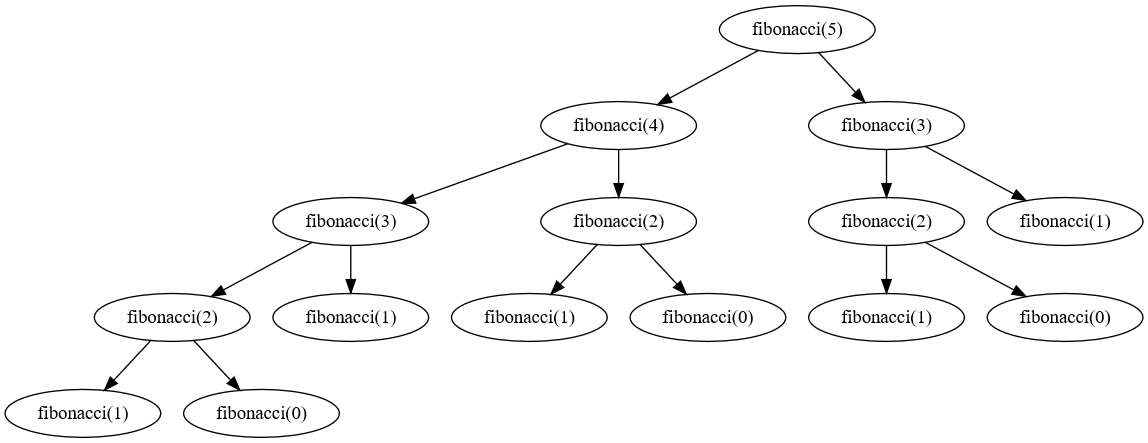
\includegraphics[width=5in]{ch-recursion/Fibonacci}
\end{figure}

For $n=5$, the \texttt{fibonacci} function is invoked 15 times total. See \url{https://oeis.org/A001595} for a function giving the number of nodes in the Fibonacci tree.

Programmers and mathematicians have discovered many techniques to compute the Fibonacci sequence more quickly. A relatively obvious improvement is \textit{dynamic programming}. Dynamic programming refers to algorithms that break a problem into subproblems and deduplicate subproblems with \textit{memoization}. In the case of Fibonacci, for all $n \ge 3$ there will be two calls to $n-2$. If the value $F_{n-2}$ can be cached then the dynamic programming algorithm can significantly reduce the amount of work needed to compute $F_n$ \cite{nayuki}.

\section{Ackermann}

The Ackermann Function is another famous recursive algorithm \cite{weissteinAckermann}.

\begin{equation*}
A(x,y) =
\begin{cases}
y+1 & \textrm{if } x=0 \\
A(x-1, 1) & \textrm{if } y=0 \\
A(x-1,A(x,y-1)) & \textrm{otherwise}
\end{cases}
\end{equation*}

$A(0,0)=1$ and invokes the Ackermann function only once. $A(1,1)$ calls $A(0, A(1, 0))$. The inner $A(1,0)=A(0,1)=2$, so the outer $A(0,A(1,0))=3$. Drawing a graph helps to visualize the calls.

\begin{figure}[hbhb]
\centering
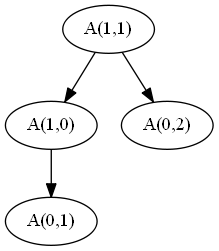
\includegraphics[height=2in]{ch-recursion/a_1_1_}
\caption{$A(1,1)=3$}
\end{figure}

$A(2,2)=7$ but requires 27 operations to compute.

\begin{figure}[H]
\centering
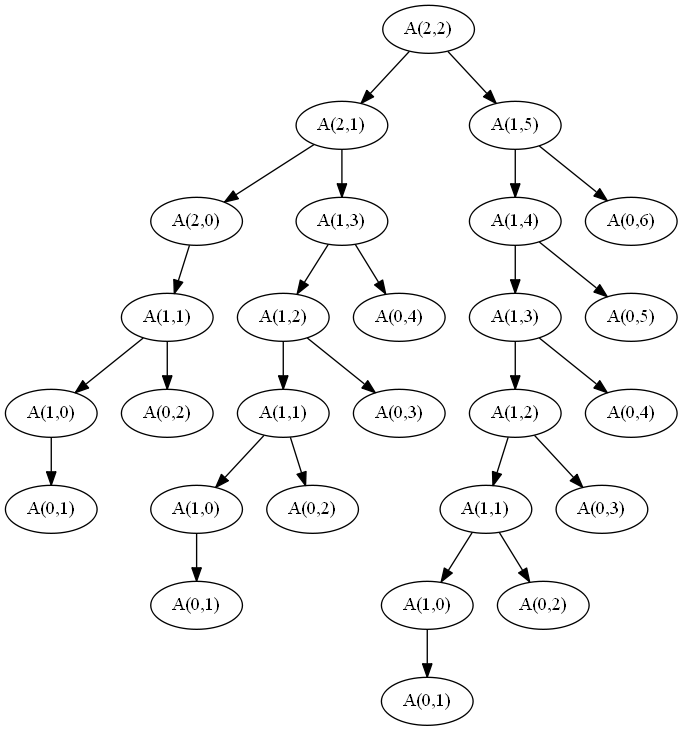
\includegraphics[height=2in]{ch-recursion/a_2_2_}
\caption{$A(2,2)=7$}
\end{figure}

$A(3,3)=61$ and requires a staggering 2432 operations to compute.

\begin{figure}[H]
\centering
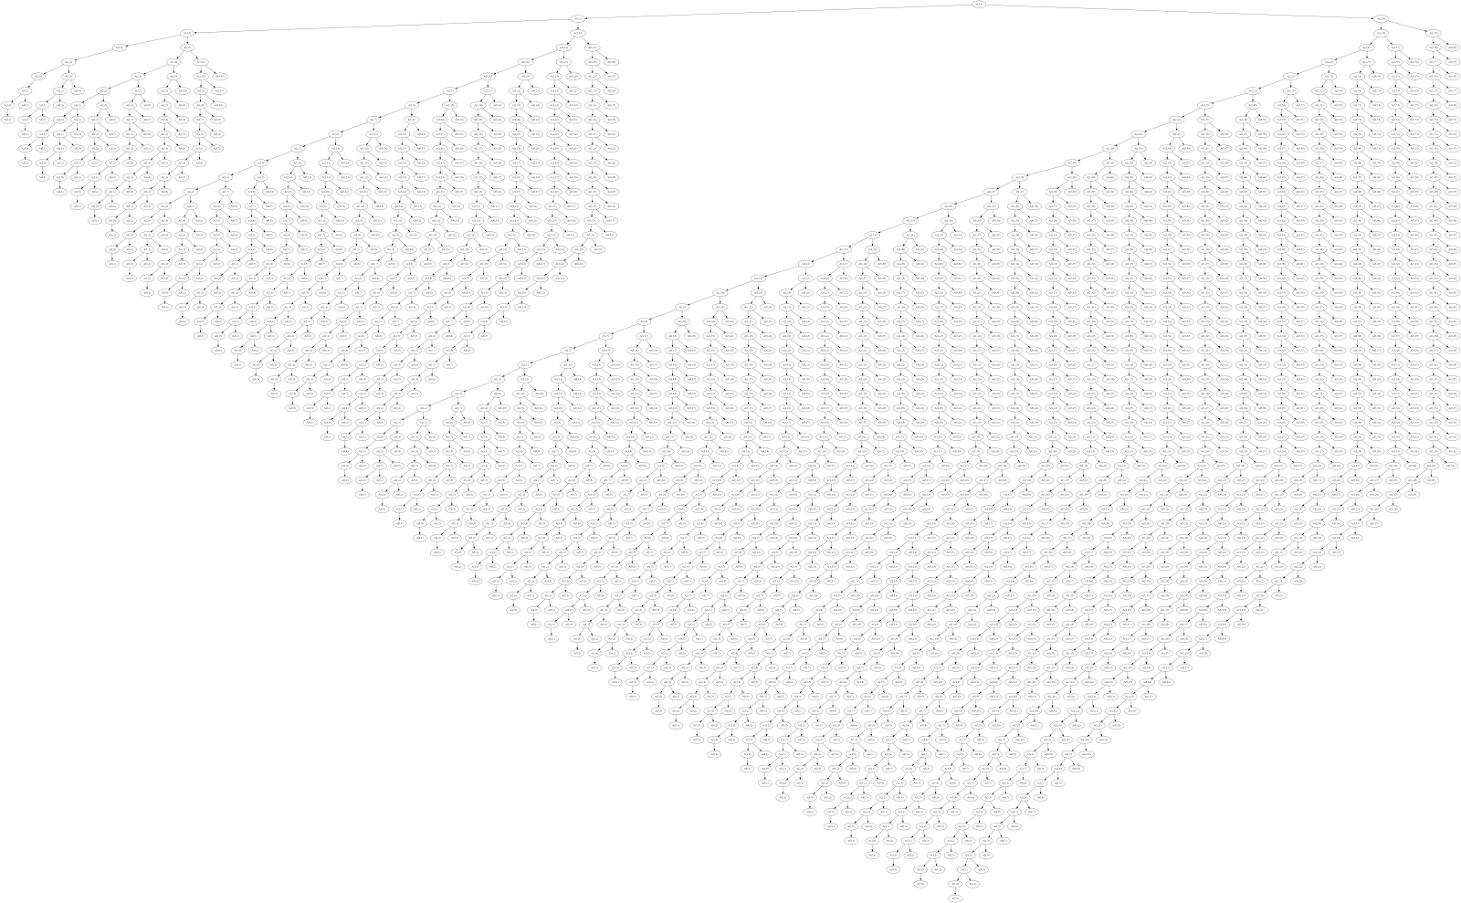
\includegraphics[width=5.5in]{ch-recursion/a_3_3_}
\caption{$A(3,3)=61$}
\end{figure}

$A(4,4)=2^{2^{2^{65536}}}-3$ --- a very large number. The Ackermann function can be considered \textit{hyperexponential}. The amount of effort necessary to compute $A(x,y)$ grows in \textit{power towers} of the form $2^{2^{2^{2^{...}}}}$ as $x$ and $y$ increase.

The Ackermann function has several interesting properties. First, the explosive growth of this function makes it practically impossible to calculate values such as $A(1000,1000)$. The universe does not have enough electrons to represent such a large number. However, observe that $x$ never increases in any of the three cases of $A(x,y)$ and $y$ only increases at a base case with no recursive step. The Ackermann function cannot enter an infinite loop. Though it is not practical to compute $A(x,y)$ for large $x$ and $y$, Ackermann is theoretically \textit{computable} for all $x,y \in \mathbb{Z}_{\ge 0}$.

Second, the Ackermann function is not \textit{primitive recursive} \cite{computerphileackermann}. That is, it cannot be rewritten using simple \texttt{while} and \texttt{for} loops. A \textit{simple} loop is not allowed to modify the exit condition --- it iterates a finite number of times and terminates.

\section{Collatz}

The Collatz problem is another famous example of recursion \cite{weissteinCollatz}. Unlike the Ackermann function, which is provably computable, it is not known if a value $a_n=1$ exists for all $a_0 \in \mathbb{Z}_{> 0}$.

\begin{equation*}
a_n =
\begin{cases}
\frac{1}{2}a_{n-1} & \textrm{for } a_{n-1} \textrm{ even} \\
3 a_{n-1} + 1 & \textrm{for } a_{n-1} \textrm{ odd}
\end{cases}
\end{equation*}

The Collatz \textit{conjecture} states that $a_n = 1$ for all positive integers $a_0$. This may make more sense with a bit of code and some examples.

\begin{lstlisting}
static void collatz(int n) {
	if (n < 1) throw new IllegalArgumentException("n < 1");

	System.out.print(n + " ");
    
	if (n > 1) {
		if ((n & 1) == 1)
			collatz(3 * n + 1); /* odd */
		else
			collatz(n >> 1);    /* even */
	} else {
		/* Terminate because a_n == 1 reached. */
		System.out.println();
	}
}
\end{lstlisting}

The above \texttt{collatz} function in Java prints space-separated terms of integer sequences generated by the Collatz function. Here are the first twenty.

\begin{lstlisting}
1 
2 1 
3 10 5 16 8 4 2 1 
4 2 1 
5 16 8 4 2 1 
6 3 10 5 16 8 4 2 1 
7 22 11 34 17 52 26 13 40 20 10 5 16 8 4 2 1 
8 4 2 1 
9 28 14 7 22 11 34 17 52 26 13 40 20 10 5 16 8 4 2 1 
10 5 16 8 4 2 1 
11 34 17 52 26 13 40 20 10 5 16 8 4 2 1 
12 6 3 10 5 16 8 4 2 1 
13 40 20 10 5 16 8 4 2 1 
14 7 22 11 34 17 52 26 13 40 20 10 5 16 8 4 2 1 
15 46 23 70 35 106 53 160 80 40 20 10 5 16 8 4 2 1 
\end{lstlisting}

The \texttt{collatz} function can be implemented in many ways. This program pedagogically uses a bit mask and bit shift. The program branches based on the last bit in the input value $n$.

All inputs $1 \le a_0 \le 20$ eventually branch to a value of 1. In fact, there is no known positive integer that does not. Could there be some value $a_0$ that does \textbf{not} lead to 1? This is an unsolved problem in mathematics. The Collatz conjecture states that there is no such value, and all positive integers input into the Collatz function will generate a finite-length sequence ending with the value 1.

The Collatz function is related to several important principles of Computer Science. First, whether the Collatz conjecture is true or false it stands as a good example of \textit{undecidability}. 

The Ackermann function has been proven to be \textit{computable} for all possible values in its domain. That is, Ackermann can never an infinite loop. By contrast, it is not known if all inputs to the Collatz function will eventually lead to 1 or not.

Alan Turing proved in his famous paper \textit{On Computable Numbers, with an Application to the Entscheidungsproblem} that it is not possible to construct an algorithm to predict whether any given decision problem, such as the Collatz function, is solvable \cite{turing1937computable}.

\chapter{Tries}

The most obvious method for storing a dictionary of words on a computer is a two-dimensional array. Each word is an array of characters, better known as a ``string,'' and an array of strings becomes a dictionary. The memory requirements for this data structure is simply the sum of all characters for each word.

An algorithm to search for the presence of a word would have to check all $n$ strings in the dictionary, stopping when the input is exhausted or a match is found. The best case scenario is that a match is found on the first attempt. The worst case requires a comparison to all $n$ elements if no match is present.

\begin{lstlisting}[mathescape]
Linear-Search (Needle $x$, Haystack $l$) {
  for each Element $y$ in $l$ {
    if $x = y$ then return true
  }  
  return false
}
\end{lstlisting}

An array of strings can be searched more quickly if the dictionary is sorted. A \textit{bisection} algorithm begins at the middle of the array. If the middle element is greater than the query then the algorithm branches to the left, making the next comparison at the $n/4$ position. If the middle element is less than the query then the algorithm branches to the right, making the next comparison at the $3n/4$ position. The algorithm terminates when the search term is found or no further bisection is possible.

\begin{lstlisting}[mathescape]
Bisection-Search (Needle $x$, Haystack $l$) {
  assume $l$ is sorted
  $n \gets |l| / 2$
  while ($n>1$) {
    if $x = l[n]$ then return true
    if $x < l[n]$ then $n \gets n - \lfloor n/2 \rfloor$ // $x$ smaller, branch left
    if $x > l[n]$ then $n \gets n + \lfloor n/2 \rfloor$ // $x$ greater, branch right
  }
  return false
}
\end{lstlisting}

Bisecting the array leads to a result in a maximum of $\log_2 n$ steps. This is much better than taking all $n$ comparisons through iteration, but there is an even faster method.

A \textit{tree} is an acyclic graph. A graph is a set of vertices and edges, typically written $G=(V,E)$. A \textit{trie} is a \textit{radix tree} where each node represents an element in a list. Each \textit{path} from the root node to each leaf constructs the lists represented in the trie.

Tries are easiest to understand if presented graphically. Figure \ref{h4} illustrates a dictionary containing four words. The terminus \texttt{\$} is used by convention to terminate strings, allowing substrings to form words of their own \cite{demainelecture}.

\begin{figure}[ht]
\centering
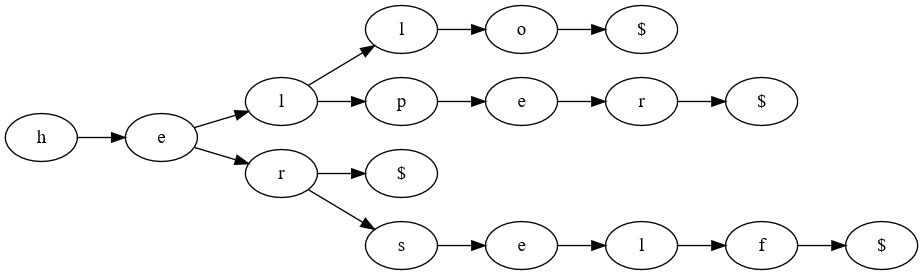
\includegraphics[width=5in]{ch-trie/hello_helper_her_herself}
\caption{A trie containing the words ``hello,'' ``helper,'' ``her,'' and ``herself''}
\label{h4}
\end{figure}

The words ``hello,'' ``helper,'' ``her,'' and ``herself'' have a combined total of $5+6+3+7=21$ characters. Many programming languages, such as C, will append a $\emptyset$ terminus to the end of a string, so in memory this may require 25 characters to represent these words as character arrays. The trie above reduces the requirement to only 17. Compression further improves as dense tries contain increasingly many words of common prefix.

Even further compression can be found if common suffixes are combined. Notice the words ``helper'' and ``her'' both end in ``r.''

\begin{figure}[ht]
\centering
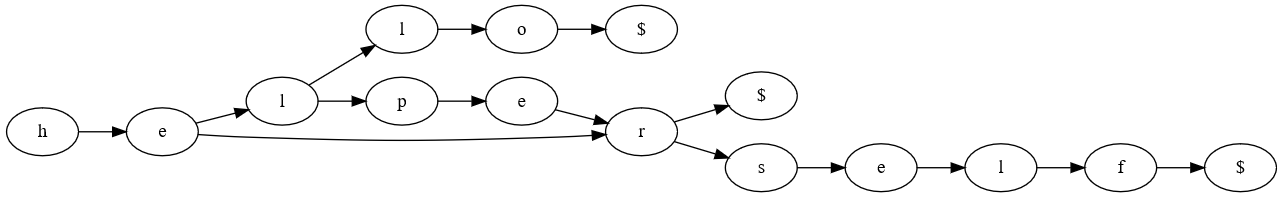
\includegraphics[width=5in]{ch-trie/hello_helper_her_herself_common_suffix}
\caption{The words ``helper'' and ``her'' share a common suffix}
\label{h4c}
\end{figure}

The common ``r'' saves only a single character in figure \ref{h4c}, but one can easily imagine the memory savings for all words ending in ``ing'' in an English dictionary.

The edges linking vertices in a trie are not free. A pointer in C could be used to connect one \texttt{struct} containing one datum to the next \texttt{struct}. On the x64, pointers are 64 bits wide --- considerably larger than a two-byte UTF-16 character. Additionally, the data structure holding a list of pointers from each vertex to the next will impose some overhead of its own. Finally, arrays often have significant speed advantages compared to other data structures due to \textit{locality of reference}. \textit{Locality}, in this context, refers to machine-dependent performance benefits when accessing close or contiguous memory locations.

Framing and machinery are important considerations when designing practical programs. Compression benefits of a trie are only realized when the tree is quite dense. Still, the search speed of a trie is practically unbeatable.

\begin{lstlisting}[mathescape]
define Trie ::= { Value $v$, Set of Tries $e$ }

Trie-Search (Word $w$, Trie $t$) {
  if $w$.Length = 0 then return true
  $x \gets$ Extract-Head($w$)
  if $\neg \exists c[c \in t.e \wedge x = c.v]$ then return false
  else return Trie-Search($w$, $c$)
}
\end{lstlisting}

This primitive-recursive algorithm steps through each letter in the word, testing if the \texttt{Trie} data structure contains this letter in its set of children. Letters are extracted from the head until no letters remain or no matching character can be found in any child vertex. Searches will require no more steps than the length of the word.

A clever technique for building tries with relatively low overhead is to use two linked lists \cite{pitts_trie}. One linked list points to nodes at the same level in the subtree. The second linked list contains all child nodes. A visualization of this approach is shown in figure \ref{trie_in_c}.

\begin{figure}[ht]
\centering
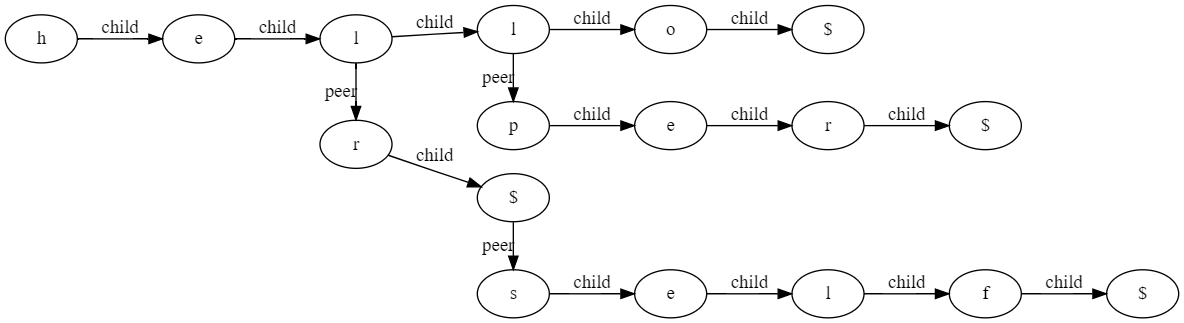
\includegraphics[width=5in]{ch-trie/hello_helper_her_herself_as_trie_in_c}
\caption{A linked-list trie with pointers to both peers and children}
\label{trie_in_c}
\end{figure}

\begin{lstlisting}
typedef struct _t {
    char c;
    struct _t * peer;   // a linked list of peers at the same level
    struct _t * child;  // a linked list of children from this node
} * trie;

trie insert(char * w, trie t) {
    if (* w == '\0') return t;
    if (t == NULL) {
        trie n = calloc(1, sizeof(struct _t));
        n->c = * w;
        n->child = insert(++w, NULL);
        return n;
    } else {
        while (t->c != * w) {
            if (t->peer == NULL) {
                t = t->peer = calloc(1, sizeof(struct _t));
                t->c = * w;
            } else {
                t = t->peer;
            }
        }
        if (t->child == NULL) {
            t->child = insert(++w, NULL);
        } else {
            insert(++w, t->child);
        }
        return t;
    }
}

void freetrie(trie t) {
    if (t->child != NULL) {
        freetrie(t->child);
    }
    if (t->peer != NULL) {
        freetrie(t->peer);
    }
    free(t);
}
\end{lstlisting}

This algorithm is easily understood using the flow chart in figure \ref{flowchart}. The \texttt{insert} function accepts a word and a trie as arguments. Both values can be null. If the word is empty then there is no further work to complete, otherwise the \texttt{insert} function extracts the first letter $c$ from the word. If the trie is null then the algorithm constructs a new trie node with value $c$. The child of this new trie will be set from the result of the next call to \texttt{insert}. If the trie was not null then the algorithm iterates through the current trie node and all of its peers. If any of these nodes match $c$ then there is no need to insert a new entry and the algorithm proceeds with the next character in the word; otherwise, the algorithm constructs a new trie node with value $c$ as a peer to the tail of the linked list of peers, then proceeds along the next value in the word as a child to the new trie containing $c$.

\begin{figure}[ht]
\centering
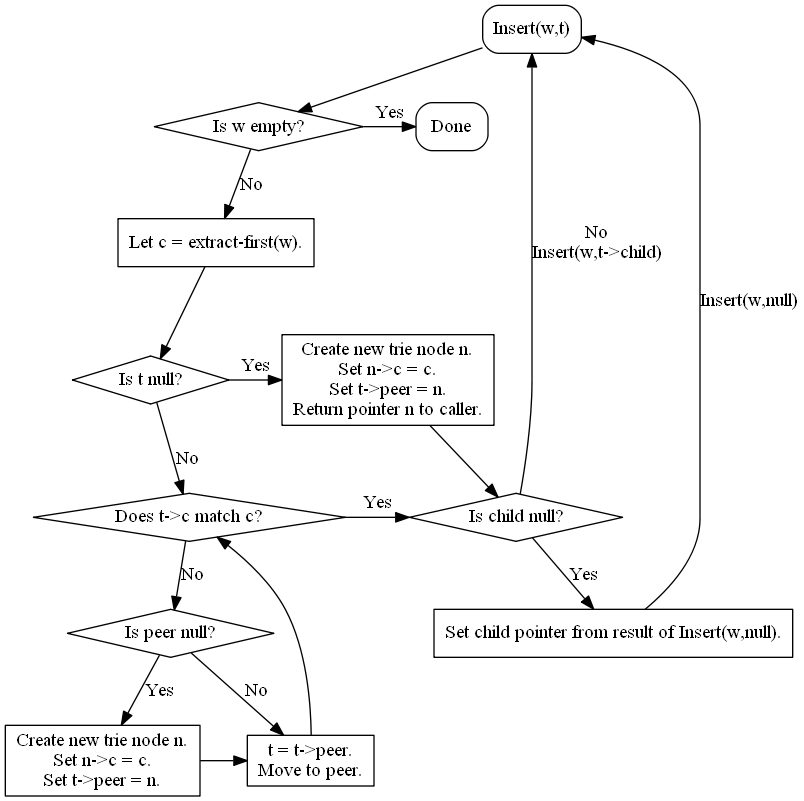
\includegraphics[width=5in]{ch-trie/flowchart}
\caption{An algorithm to insert letters into a trie based upon two linked lists}
\label{flowchart}
\end{figure}

Tries can be used to implement routing tables in computer networking \cite{nilsson1998}. A trie might hold network prefixes and associated next-hop interfaces or addresses. Route lookups will require $O(m)$ operations (where $m$ is the length of the address) regardless of the number of entities in the trie.

A trie containing IP addresses is a special case of a trie because the data structure is a bit string. The elements of the trie can contain only the values 0 or 1. This invariant of the binary trie reduces its complexity; there is no need for a linked list of peers. The below reference implementation uses a two-element reference array to link a parent node to its left and right children. \texttt{child[0]} references the left child, taken when the value at that position contains the value 0. \texttt{child[1]} references the right child is taken when the digit at the appropriate position equals 1.

The root node is special. If may contain a next-hop interface but it has a height of 0. This is consistent with IP routing, where a route \texttt{0.0.0.0/0} is used as a default route. If a route lookup fails then the \texttt{lookup} function returns the next-hop of the default route (if any). The program could be extended to support \textit{recursive routing} where an IP address is given as the next-hop for a route.

Though not implemented, the trie data structure could be easily modified to support deletion of a route; simply unlink the \texttt{iface} next-hop to remove a route. Though perhaps desirable, it is not strictly necessary to delete the intermediate trie nodes themselves.

The sample trie data structure presented as a simple routing table provides two key operations: insertion and lookup. Both functions are recursive in definition and both run in $O(m)$ time. Iteration through a trie is possible but inefficient.

If the values in the radix of a trie form a total order then it is possible to find the maximal and minimal elements by repeatedly following the maximal or minimal nodes in $O(m)$ time. This is still not as efficient as $O(1)$ queue operations with a double-ended queue. In a trie of $n>2$ elements, elements $t_k$ where $1 \le k \le n-1$ cannot be deterministically accessed. The trie is \textit{not} a general-purpose data structure and should not be used if arbitrary access is required.

\begin{lstlisting}
public class Route {
    
    private String iface;
    private Route child[];
    
    public static Route root = new Route();
    
    private Route() {
        child = new Route[2];
    }
    
    static void insert(int ip, int prefix, String iface) {
        if (prefix == 0) {
            root.iface = iface;
        } else {
            root.insert(ip, prefix, iface, 1);
        }
    }
    
    private void insert(int ip, int prefix, String iface,
                        int current) {
        if (prefix < current) {
            this.iface = iface;
        } else {
            int value = (0b10000000_00000000_00000000_00000000 >>>
                        (current-1)) & ip;
            value = (value == 0) ? 0 : 1;

            if (child[value] == null) {
                child[value] = new Route();
            }
            
            child[value].insert(ip, prefix, iface, current + 1);
        }
    }
    
    @Override
    public String toString() {
        return ((iface == null) ? "" : iface + " ") + "("  + child[0]
                + "," + child[1] + ")";
    }
    
    private void print(int ip, int prefix) {
        if (this.iface != null) {
            System.out.println(intIPtoString(ip) + "/" + prefix 
            + "\t\t" + this.iface);
        }
        if (this.child[0] != null) {
            this.child[0].print(ip, prefix + 1);
        }
        if (this.child[1] != null) {
            ip |= (0b10000000_00000000_00000000_00000000 >>> prefix);
            this.child[1].print(ip, prefix + 1);
        }
    }
    
    static String intIPtoString(int ip) {
        int o1 = (ip >>> 24);
        int o2 = (ip >>> 16) & 0xff;
        int o3 = (ip >>> 8) & 0xff;
        int o4 = (ip) & 0xff;
        return o1 + "." + o2 + "." + o3 + "." + o4;
    }
    
    static String lookup(int ip) {
        String r = root.match(ip);
        return (r == null) ? root.iface : r;
    }
    
    private String match(int ip) {
        int value = (ip >>> 31);

        if (child[value] != null) {
            return child[value].match(ip << 1);
        } else {
            return iface;
        }
    }
}
\end{lstlisting}

\chapter{Caesar and Vigen\`ere Cipher}

Symmetric cryptography requires a shared secret key to encrypt and decrypt a plaintext message $M$ to a ciphertext message $C$. Modern examples of symmetric cryptosystems include 3DES, AES, and RC4. As these modern ciphers are very complex, it is useful to study older and simpler ciphers. Two well-known ciphers from history are the Caesar cipher and Vigen\`ere cipher.

The Caesar cipher shifts characters in $M$ by some fixed distance $k$. Modulo operations allow characters to overflow to the first letter in the alphabet. Each letter in a word gets encoded by the same amount.

\begin{equation}
E(M, i, k) = (M_i + k) \mod{26}
\end{equation}

Decryption uses the same algorithm with $-k$ or, equivalently, $26 - k$.

\begin{equation}
D(C, i, k) = (C_i - k) \mod{26}
\end{equation}

Users of this cipher should omit spaces entirely to prevent easy guesses. For example, the ciphertext ``\texttt{pmzi psrk erh tvswtiv}'' contains a three-letter word. Two common three-letter words in English are ``the'' and ``and.'' Guessing that $E(\texttt{the}, k) = \texttt{erh}$ reveals a contradiction: the space between ``t'' and ``e'' is 15 but the space between ``h'' and ``n'' is 6. $k$ may be 6 or 15, but $\not \exists k [E(\texttt{the}, k) = \texttt{erh}]$.

Removing spaces goes a long way to remove lucky guesses but there are other methods of cryptanalysis. Frequency analysis is a classic technique of identifying the most common characters in a message and guessing which of the most common letters in a language they may be. The ciphertext ``\texttt{johunldljhuilsplclpu}'' contains several letters ``l,'' which could stand for any character but are most likely to stand for ``e,'' ``t,'' ``a,'', ``o,'' or ``i.''

\begin{lstlisting}[caption={A C function to encrypt a string using the Caesar cipher},captionpos=b]
void caesar(char * message, int length, int key) {
    int i = 0;
    while (message != NULL && i < length && message[i] != '\0') {
        if ('a' <= message[i] && message[i] <= 'z')
            message[i] = ((message[i] - 'a' + key) % 26) + 'a';
        i++;
    }
}
\end{lstlisting}

Brute force is a viable option for attacking the Caesar cipher even by hand; with an alphabet of only 26 letters an attacker can simply attempt all 26 possibilities against a reasonable segment of text.

The Vigen\`ere cipher uses a similar mechanism as the Caesar cipher with a minor variation: Vigen\`ere derives encipherment keys by rotating positions in a word. For example, to encrypt a word ``\texttt{test}'' with the key ``\texttt{abcd}'' then the ciphertext becomes ``\texttt{tfuw}.'' An encryption key ``a'' rotated ``t'' by zero positions, but the encryption key ``d'' rotated ``t'' to ``w.''

\begin{lstlisting}[caption={A C function to encrypt a string using the Vigen\`ere cipher},captionpos=b]
void vigenere_e(char pt[], int length, char key[], int key_length) {
    int x = 0;
    for (int i = 0 ; i < length ; i++) {
        if ('a' <= pt[i] && pt[i] <= 'z') {
            int shift = key[x % key_length] - 'a';
            pt[i] = (char) (((pt[i] - 'a' + shift) % 26) + 'a');
            x++;
        }
    }
}
\end{lstlisting}

Cryptanalysis of messages enciphered by Vigen\`ere requires a different approach than the Caesar cipher. Take for example an extremely controversial poem from the year 1899:

% https://daniel-hug.github.io/longest-repeated-substring/

\begin{lstlisting}[caption={A controversial poem from 1899 encrypted by a Vigen\`ere cipher},captionpos=b]
dizp cc zrm lsqgk wic'd jhxnmc-
dmaj pwgep gno jtdb lk lztpl-
tu cmco gbab adya gu ofxwm
gu cmggm luez rlxgofmh' ymrj
dw llqg ox ptldl nkzcpaf
ux nafbgkbms qwyq kvs hqyj-
iwjc vrc-mijrpg, yetapv ckyxapa,
ugvn spdvr kvs siyl mpxwl
ggum ja buk gpxem zgx'a qfzqkx
qc aigoovrp bb glqsp
bb boqa epr zrztlb bl dmgcwe
gxl rsmpq dpt dpbc yn ecqqk;
lg dama yzmtnp ntn axxxyk
kv wfvqxol itury wisp xygsv
iz arku iczbukb'a ecwsod
ico ebxu iczbukb'a vlqa
zkst fx gno ewtbr skv'h mcejov-
pyl ekkx wta brn zthiej:
dpt mtnso wu epbyo gt mmgzoz
ism ugdm dq buucm np ohgbl-
ism pxi wu swfzc gt sczuez
(ps ayugtn) ew gno txrpg:
"crg qcwhmrb np cf lbwb mwajkot,
zce rydto mtezbxlv aoqpi?"
eixk ex ism jnsbt xia'y lcgoma-
nkdt owak gqis kuovlxdp qgia-
ism yoqpiwg cxynupzrj vijcmy,
zrm tlal, axogfltkn xglqfk.
mwbpa aug, bd dmnxmp nzce skvwzwq
zrzdfou gvt ism gnkvzwmfy impca,
puvl-toorj gqis lrgb-jdfouz gqhowz,
zrm yfltsovi zn luez epmey!
\end{lstlisting}

A close look at the ciphertext reveals a repeated substring ``\texttt{iczbukb}.'' In fact, the longest repeating substring is actually ``\texttt{u iczbukb'a}.'' The distance between the first ``\texttt{iczbukb}'' and second is 14 characters. 14 could be a multiple of the key length.

Attacking the word ``\texttt{iczbukb}'' can be made simple by guessing common English strings. For example, the substring ``\texttt{str}'' occurs very frequently.

\begin{lstlisting}[caption={A C function to decrypt a string using the Vigen\`ere cipher},captionpos=b]
void vigenere_d(char pt[], int length, char key[], int key_length) {
    int x = 0;
    for (int i = 0 ; i < length ; i++) {
        if ('a' <= pt[i] && pt[i] <= 'z') {
            int shift = key[x % key_length] - 'a';
            pt[i] = (char) (((pt[i] - 'a' - shift + 26) % 26) + 'a');
            x++;
        }
    }
}
\end{lstlisting}

Deducing that the key could be of length 1, 2, 7, or 14 characters by assuming the repeated substrings ``\texttt{iczbukb}'' represent the same plaintext, the attacker can now apply brute force or attempt common substrings from the English language.

The string ``\texttt{str}'' occurs regularly in English. Attempting to decrypt the letters ``\texttt{icz},'' ``\texttt{czb},'' ``\texttt{zbu},'' ``\texttt{buk},'' and ``\texttt{ukb}'' decrypt to ``\texttt{qji},'' ``\texttt{kgk},'' ``\texttt{hid},'' ``\texttt{jbt},'' and ``\texttt{crk}'' by shifting the key ``\texttt{str}'' from left to right. Of these, only the output ``\texttt{hid}'' sounds plausible. Additional candidate substrings to try might include ``\texttt{ing},'' ``\texttt{ion},'' ``\texttt{ace},'' etc. With a computer it is reasonable to attempt all two- and seven-character words and search for recognizable words in the output.

The combination of several words to form a 14-character pass phrase offers greater resistance to dictionary attacks. Still, an attacker could pad dictionary words with one or more letters ``a'' (which leaves the plaintext unchanged) and continue searching for legible words.

The Vigen\`ere cipher was used in the American Civil War. Strangely, Confederate States of America exercised very poor communications security by repeatedly reusing a small number of key phrases. This demonstrates Kerckhoff's principle that the keys are the backbone of cryptographic strength, not the obscurity or cleverness of the algorithm.

By using a random key of length equal to the plaintext the cipher becomes a \textit{one-time pad} impervious to cryptanalysis.

\chapter{Proxies}

\section{Security Models}

Clark and Wilson contrasts military and commercial security models in an influential paper that has become known as Clark-Wilson \cite{clark-wilson}. The military model is, in essence, the Bell-LaPadula secure computer system \cite{bell1976secure}. The Bell-LaPadula model prioritizes confidentiality and can be understood as ``read-down, write-up.'' That is, a high confidentiality system may write to higher confidentiality systems but not read from them, and it may read from lower confidentiality systems but not write to them. The commercial model described by Clark-Wilson is similar to the Biba integrity model \cite{biba1977integrity}. Biba takes the opposite approach as Bell-LaPadula; high integrity systems may write to low integrity systems but the opposite is not permitted.

The well-formed transaction is essential to maintaining data integrity. The user generally does not have direct write access to storage. Instead, programs are assigned privilege to read and write to storage. The permissions of the user dictate what programs that user may invoke. These programs are responsible for reading and writing data in the correct format and at the user's privilege level. This model is distinct from Orange Book controls that emphasize the user's ability to read or write to data directly.

The command \texttt{passwd} in Unix and Linux is an example of a program that executes well-formed transactions on behalf of a user against a data location that the user does not have write access to. Password hashes are stored in \texttt{/etc/shadow}. \texttt{/etc/shadow} is typically neither readable nor writable to users. To change a password a user invokes the \texttt{passwd} program. \texttt{passwd} is configured with the \texttt{setuid} bit set (\url{https://docs.oracle.com/cd/E19683-01/816-4883/secfile-69/index.html}). The \texttt{setuid} tells the operating system to execute the program with the privilege level of the program file's owner.

\begin{lstlisting}[caption={The \texttt{s} in \texttt{rws} indicates the \texttt{setuid} bit is active.}]
$ which passwd
/usr/bin/passwd
$ ls -al /usr/bin/passwd
-rwsr-xr-x. 1 root root 30768 Nov  3  2015 /usr/bin/passwd
\end{lstlisting}

Most computing systems read and write to resources through intermediate programs. A user entering data into web-based application typically has no access to the back-end database. It is the web application running on a web server that accesses the database, and even this access might be indirect.

Clark-Wilson formalizes the concept of an \textbf{Integrity Verification Procedure}, or IVP, acting as a formatter or filter between users and transactions. Clark-Wilson explores rules and policies that an IVP may impose on transactions to enhance either or both the confidentiality and integrity of the information system.

\section{Proxy Servers}

A proxy server is an application or appliance that brokers HTTP connections on behalf of users. Proxy servers can be explicitly configured in the browser or transparently positioned in the network. Modern proxy servers support HTTPS but this architecture requires cryptographic planning and configuration.

The simplest HTTP proxy server is nothing more than a TCP socket listening for incoming connections. The proxy server will require at least two TCP sockets to broker client connections. The first is a server socket listening for incoming connections from clients. The second is an outbound client connection initiated on behalf of the original client.

\begin{lstlisting}[caption={A simple HTTP proxy written in PowerShell},label=psproxy]
# Open TCP server socket listening on all network interfaces.
# This works for IPv4 and IPv6.
$port = 32768
$listener = [System.Net.Sockets.TcpListener] $port
$listener.start()

# this only works for a single client
$client = $listener.AcceptTcpClient()

while ($true) {
  $stream = $client.GetStream()
  [byte[]] $bytes = New-Object byte[] 1024
  if ($stream.Read($bytes, 0, 1024) -gt 0) {
    [System.Text.Encoding]::ASCII.GetString($bytes)

    # This encoding assumption is unsafe.
    # What if the content is UTF-8 instead of ASCII?
    $encoding = [System.Text.Encoding]::ASCII;
    $url = $encoding.GetString($bytes).split(" ")[1]

    $proxy = (Invoke-WebRequest -Uri $url)

    $encoder = New-Object System.Text.ASCIIEncoding
    $bytes = $encoder.GetBytes($proxy.RawContent)
    $stream.Write($bytes, 0, $bytes.Count)
  }
}

$client.Close()
\end{lstlisting}

Listing \ref{psproxy} is a simple HTTP proxy server written in PowerShell. This program binds to TCP port 32768 on all of the host's network interfaces. Implicitly, this will work for both IPv4 and IPv6. This proxy server can only service a single client. The proxy server requires no privilege on a typical Windows host.

To command-line client might connect to a web site through this proxy using the command \texttt{Invoke-WebRequest http://neverssl.com -Proxy http://127.0.0.1:32768}. Like \texttt{curl} and \texttt{wget}, PowerShell's \texttt{Invoke-WebRequest} accepts a proxy server specified at the command-line. If no proxy server is specified then the system-wide configuration is used.

A proxy server, brokering HTTP connections on behalf of clients, may modify data in motion. This provides several opportunities.

First, a proxy server may cache data that has been repeatedly sent over the network. The proxy server will almost invariably serve cached content significantly faster distant web servers. Overall network utilization may be decreased through de-duplication. Caching can cause problems, though. Content on the modern web regularly changes, and proxy servers should periodically delete cached copies of websites to allow changes to reach users. Some web operators, notably YouTube, require network operators to not cache traffic for business reasons. Finally, caching data creates confidentiality and privacy concerns. A proxy server should not cache sensitive information and serve it to the wrong user.

Another capability available through proxy servers is to filter content. A network operator seeking to block access to certain websites might use a proxy to do so. Restricting network access can be achieved at the network layer as well but in practice IP address filters are more difficult to troubleshoot and maintain than lists of domain names.

A proxy server might filter not only by destination host but file type. Security-conscious network operators might restrict HTTP clients from downloading \texttt{.exe} files. Likewise, data loss prevention policies might, for example, restrict network users from uploading \texttt{.pdf} files. Enforcing these policies at the proxy server therefore acts as the Integrity Verification Procedure (IVP) described in Clark-Wilson.

More intrusive proxy servers might inspect the contents of transit traffic for virus signatures, check the hashes of files or strings against lists, or check HTTP parameters for potential SQL injection. The most advanced proxies can use machine learning and even computer vision to recognize and act on interesting traffic.

The use of a proxy server hides client addresses from external websites. Concealing client information is widely perceived as a benefit of deploying Network Address Translation (NAT) with IPv4 private IP addresses, but the same result is easily achievable on IPv6 with a proxy server. The presence of a proxy server may be adversely impacted if the proxy server becomes unavailable.

Conceptually, a proxy server used in HTTP is not conceptually different from any IVP. A proxy server brokers connections on behalf of clients. It can enforce policy by caching, monitoring, filtering, or modifying transit traffic. Servers may or may not be alerted that client connections are being brokered. All brokering technologies imply confidentiality and privacy concerns.

\chapter{Queues and Stacks}

\section{Queues}

A \textbf{queue} is an \textit{abstract data structure} that models a first-in/first-out (FIFO) insertion and removal model \cite{Aho:1992:FCS:114768}. Only the \texttt{enqueue(E)} and \texttt{dequeue()} operations are strictly defined. Elements are removed in the same sequence they were added.

\section{Stacks}

A closely related abstract data structure is the \textbf{stack}. A stack models a first-in/last-out (FILO) insertion and removal model. The \texttt{push(E)} and \texttt{pop()} operations add and remove elements from the stack. Elements are removed in the opposite sequence they are added.

\section{Deques}

A double-ended queue, or \textbf{deque} (pronounced ``deck''), allows extractions from both ends of the data structure. The operations of a deque are \texttt{add(E)}, \texttt{head()}, and \texttt{tail()}.

\section{Running Time}

\section{Implementation}

Each of these data structures can be modeled in several ways.

{\huge todo: explain different approaches (array, linked list, binary tree), provide sample code for each in Java instead of C, and give a table contrasting asymptotic runtimes of each.}

\begin{lstlisting}
#include<stdio.h>
#include<stdlib.h>

typedef struct _q {
  int i;
  struct _q * last, * next;
} * dlink;

struct _q _dummy;
dlink dummy = &_dummy;

void q_add(int i) {
  dlink l = calloc(1, sizeof(dlink));
  l->i = i;
  if (dummy->next == NULL) {
    dummy->next = dummy->last = l;
    l->next = l->last = dummy;
    } else {
    l->next = dummy;
    l->last = dummy->last;
    l->last->next = l;
    dummy->last = l;
  }
}

int q_head() {
  if (dummy->next == NULL)
    return -1;

  dlink r = dummy->next;
  int i = r->i;
  dummy->next = r->next;
  r->next->last = dummy;
  free(r);
  return i;
}

int q_tail() {
  if (dummy->last == NULL)
    return -1;

  dlink l = dummy->last;
  int i = l->i;
  dummy->last = l->last;
  l->last->next = dummy;
  free(l);
  return i;
}

void destroy() {
  dlink d = dummy;
  while (d != NULL && d != dummy) {
    d = dummy->next;
    free(dummy->last);
  }
}

int main() {
  atexit(destroy);
  int i;
  for (i = 0 ; i < 10 ; i++) {
    q_add(i);
  }

  /* non-destructive iteration through queue */
  dlink d = dummy->next;
  while (d != dummy) {
    printf("%d ", d->i);
    d = d->next;
  }
  printf("\n");

  /* backwards iteration through queue */
  d = dummy->last;
    while (d != dummy) {
    printf("%d ", d->i);
    d = d->last;
  }
  printf("\n");

  /* alternate between extracting from the head and tail */
  for (i = 0 ; i < 10 ; i++) {
    printf("%d ", (i & 1) ? q_head() : q_tail());
  }
  printf("\n");
}
\end{lstlisting}

\chapter{High Availability}

\chapter{Radio Wave Propagation}

Velocity is the rate at which displacement changes.

\begin{equation}
v = \frac{d}{t}
\end{equation}

The speed of light, $c$, in a vacuum is approximately 300 million meters per second.

\begin{equation}
c = 3 \times 10^8 \si{\meter}/\si{\second}
\end{equation}

We usually think of velocity in terms of a total displacement divided by total time. However, there are alternative ways to think about this concept. Suppose an object is displaced by $x$ meters for 50 times in one second then $v = 50x m/s$. The rate is not expressed to us in seconds, but by unitless cycles per second. The unit for these cycles is the Hertz.

\begin{equation}
\frac{1}{1 \si{\second}} = 1 \si{\second}^{-1} = 1 \si{\hertz}
\end{equation}

When considering velocity in terms of small intervals of time we use the symbol $\lambda = d$ to denote wavelength. Wavelength is the displacement during each cycle. Time, when expressed in Hertz, is inversely related to frequency $f = 1/t$.

\begin{equation}
v = \lambda f = \frac{d}{t}
\end{equation}

Electromagnetic signals radiate at the speed of light. Frequency is useful to distinguish signals, and the many frequencies have very different behaviors. The International Telephone Union (ITU) classify frequencies into logarithmic bands. Each band has relative strengths and weaknesses that influence usability. 

\begin{center}
\begin{tabular}{c | c | c}
Name & Frequency & Wavelength \\
\hline
High Frequency (HF) & 3 -- 30 \si{\MHz} & 10 -- 100 \si{\meter} \\
Very High Frequency (VHF) & 30 -- 300 \si{\MHz} & 1 -- 10 \si{\meter} \\
Ultra High Frequency (UHF) & 300 -- 3000 \si{\MHz} & 0.1 -- 1 \si{\meter} \\
Super High Frequency (SHF) & 3 -- 30 \si{\GHz} & 1 -- 10 \si{\cm} \\
Extremely High Frequency (EHF) & 30 -- 300 \si{\GHz} & 1 -- 10 \si{\mm}
\end{tabular}
\end{center}

VHF is a useful band for portable radios operating at land, sea, and sky. Broadcast radio operates in this band. A powerful and well-positioned radio station can easily broadcast signals to listeners 50 miles away. Smaller amplifiers mounted in military and police vehicles, boats, and aircraft can make effective use of this band over several miles in urban terrain. VHF is effective for line-of-sight communications. No band is entirely impervious to interference or attenuation but VHF tends to work well in many settings. On the other hand, the small size of the band limits the amount of data that can be used by any given station.

Antennas operate most effectively and efficiently when they have a length equal to $\lambda$, $\lambda/2$, or $\lambda/4$. Listeners to FM radio station 100.0 seeking a full-wavelength antenna finds

\begin{equation}
\lambda_{100.0 \si{\MHz}} = \frac{3 \times 10^8 \si{\meter}/\si{\second}}{100.0 \times 10^6 \si{\hertz}} = 3 \si{\meter}
\end{equation}

The FM radio will operate efficiently at a half wavelength. Radios use a coiled wire to tune the effective length of their antenna.

A transmitting antenna can be shaped to influence the radiation pattern. A typical vertical antenna is said to be omnidirectional but a ``cone of silence'' always extends from the tip. Antennas can be shaped into a ``vee'' shape, slope, and square to increase signal gain in a particular direction.

UHF is a useful band in everyday life. Microwave communications, cell phones, Wifi, Bluetooth, GPS, and military satellite radio operate in this band. UHF provides a larger spectrum and therefore more bandwidth than VHF, but it does not resist attenuation as effectively. Long-range UHF signals require more gain than VHF.

Cell phone networks have good coverage thanks only to the dense proliferation of towers. A handset does not have a powerful enough antenna to punch through several buildings or subway tunnels. Communications smoothly transition from one tower to the next thanks to sophisticated routing technologies designed for this purpose.

SHF contains the C, X, and Ku bands and most of Ka. (These lettered designations are defined in Institute of Electrical and Electronics Engineers standards). Like UHF, SHF attenuates easily if not equipped with high-gain antennas. 

Demand for bandwidth in SHF has drawn both armies and home users to EHF. The 2.4 \si{\GHz} and 5 \si{\GHz} bands used in 802.11a, b, and g networks were notoriously crowded by overlapping channels and overpowered devices. Modern 802.11ad Wifi operates at 60 \si{\GHz} and promises to offer non-overlapping, wide channels to large numbers of nearby users.

We intentionally leave HF for last. HF is special. HF requires large antennas and offers little bandwidth. Line-of-sight communications are feasible but offer few advantages over VHF. HF has a magical property that gives it a unique position in the hierarchy. HF signals can reflect off of the ionosphere back to the earth. A small HF radio can communicate with other small radios on the opposite end of the globe. Doing so requires skill, planning, and luck. The frequency and power of signals that can be reflected by the ionosphere depends on the time of day. The sun charges the layers of the ionosphere during the day and these layers discharge during the night.

Citizens band (CB) radio operates at 27 \si{\MHz}. The practice of using ``skywaves'' to propagate signals against the ionosphere is known as ``skip shooting.'' This practice is technically illegal and relatively unusual for CB radio but it is very common in the amateur ``ham'' radio community. Highly directional signals from an HF radio are therefore uniquely difficult to jam than any other band. In a war between great nations there may be few alternatives.

\chapter{Directed Acyclic Graphs}

Synchronous Optical Networking (SONET) is a communications technology for wide area networking. SONET nodes require average clock rates that are nearly equal (\textit{pesiochronous}) to communicate effectively. The node can reference an external timing source, an internal clock, or receive timing from adjacent nodes. When a SONET node receives time from another SONET node this is called \textit{line timing}.

SONET nodes can transitively receive line timing. Suppose a network of five SONET nodes $\{A, B, C, D, E\}$ communicates across a Unidirectional Path Switched Ring (UPSR). Each segment in the path has two Optical Carrier (OC-N) links operating in either working or protection states.

\begin{figure}[H]
\centering
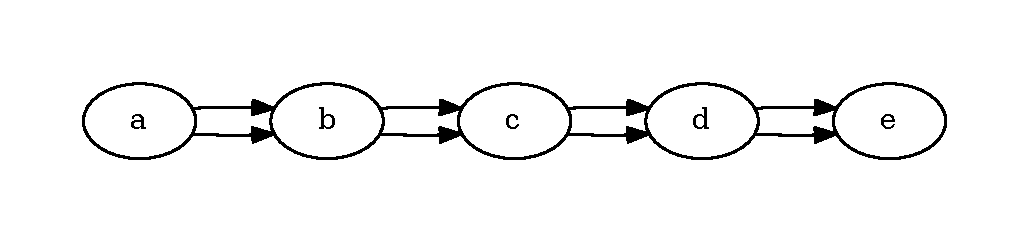
\includegraphics[width=\columnwidth]{figures/abcde}
\caption{A UPSR where nodes $B$, $C$, $D$, and $E$ each receive line timing from node $A$}
\end{figure}

Node $A$ can receive timing from an external source and then provide line timing to $B$, $B$ to $C$, $C$ to $D$, and finally $D$ to $E$. The integrity of line timing is expected to degrade as the distance from a reliable clock increases. The Network Time Protocol (NTP) solves this problem by assigning a stratum number to each device \cite{rfc1305}. Atomic clocks are assigned stratum level 0. Each device receiving time from another assigns itself a stratum level one greater than the lowest reachable source. Devices may synchronize to multiple NTP devices, and devices at the same stratum may peer with one another.

SONET timing contains a similar stratified Biba Integrity Model as NTP \cite{biba1977integrity}. A reliable timing source, such as a fixed GPS, is considered ``PRS'' at stratum 1. Less reliable timing is assigned ST2 (stratum 2), ST3, ST3E, ST4, and STU (synchronized, traceability unknown).

Configuration errors or system failures can result in timing loops. A timing loop may or may not cause device alarms or network outages. Figure \ref{loop} shows an anonymized but real SONET topology (the arrow points to the timing source). In this network, nodes $B$ and $G$ were initially deployed with external timing sources synchronized to GPS. Each node was configured to synchronize to the other if the external timing source failed. The external timing sources failed at both locations $B$ and $G$ and the nodes attempted to receive line timing from one another. This state caused alarms but did not result in an outage. 

\begin{figure}
\centering
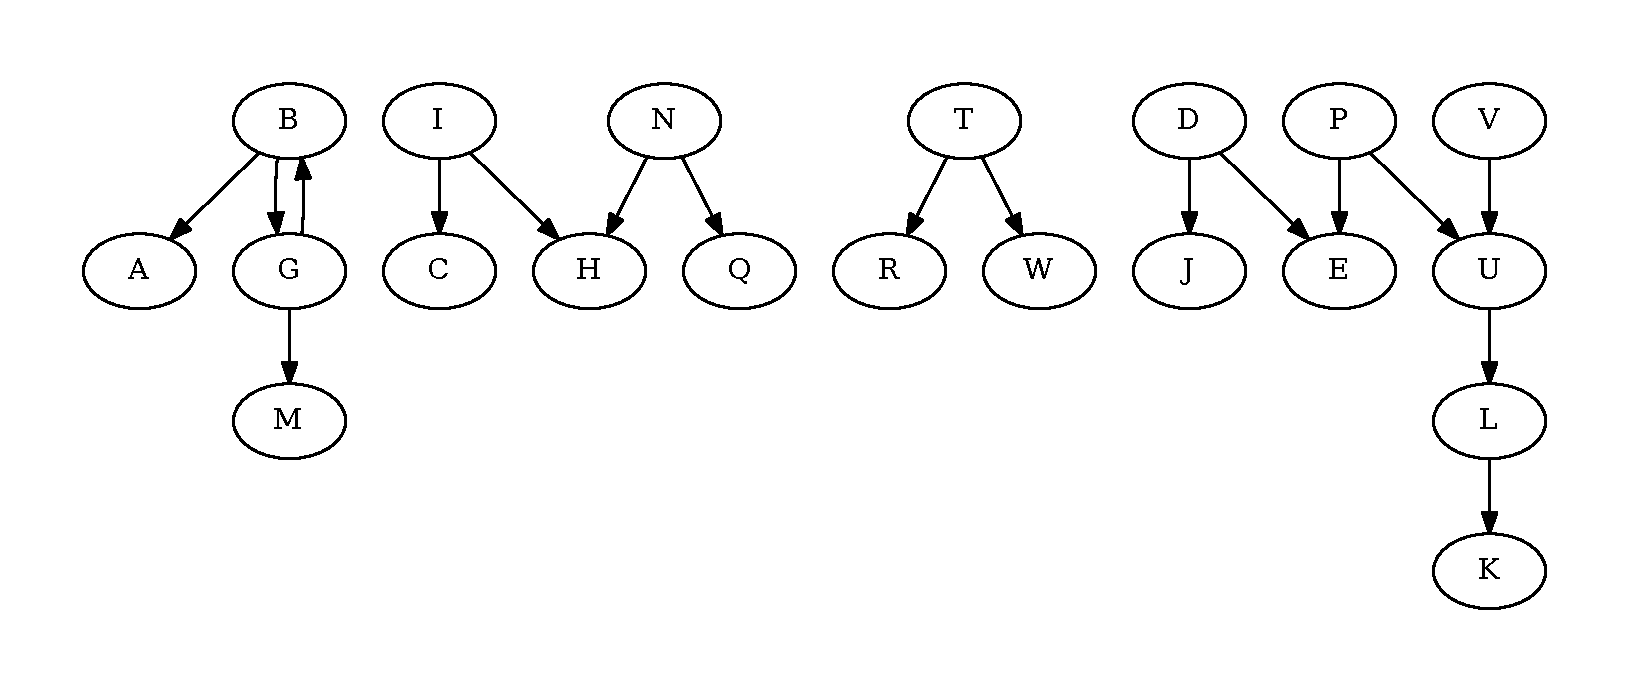
\includegraphics[width=\columnwidth]{figures/loop}
\caption{A SONET network containing a timing loop between nodes $B$ and $G$}
\label{loop}
\end{figure}

Reconfiguring device $B$ to receive timing from nodes $A$ and $H$ cleared alarms and reduced the probability of a timing-related outage. As shown in figure \ref{noloop}, the resulting topology is a \textit{directed acyclic graph}.

\begin{figure}
\centering
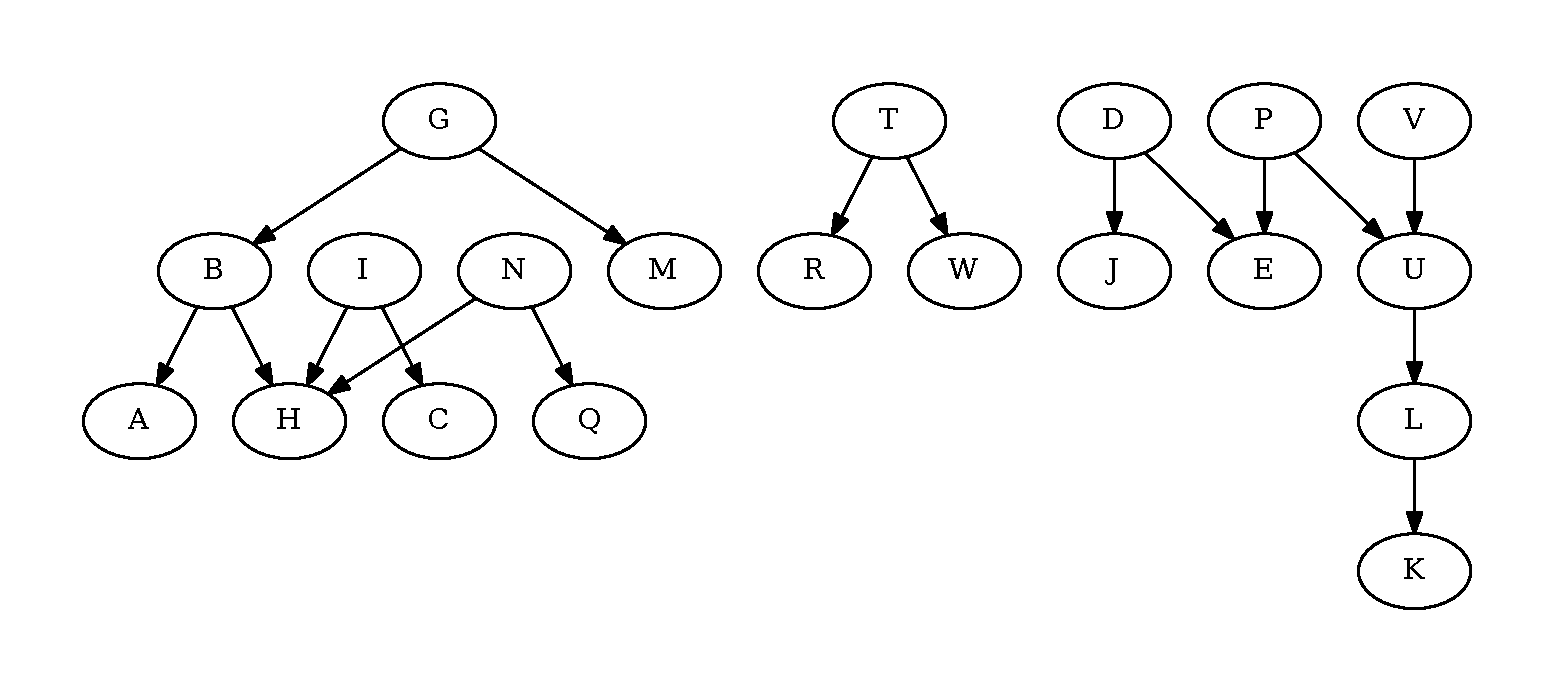
\includegraphics[width=\columnwidth]{figures/noloop}
\caption{A directed acyclic graph}
\label{noloop}
\end{figure}

Depth-First Search (DFS) is an algorithm for traversing a graph \cite{Aho:1992:FCS:114768}. DFS \textit{colors} vertices to track those that have and have not been explored. 

A simple DFS algorithm begins at some vertex $u$, colors $u$ explored, and recursively explores each unexplored adjacent vertex $v$. A modified algorithm will be shown later.

\begin{lstlisting}[columns=fixed,caption={A simple DFS function of two colors},label={2color}]
static void dfs(Map<Integer, Set<Integer>> g,
                Set<Integer> visited, int u) {
  visited.add(u);
  for (Integer v : g.get(u)) {
    if (!visited.contains(v)) {
    dfs(g, visited, v);
  }
}
\end{lstlisting}

The algorithm shown in listing \ref{2color} accepts a graph $g$ as a map. The map key, in this example, is an integer uniquely identifying a vertex. The map value is an edge set representing the out-edges from that vertex. Notice that this algorithm does not explicitly color nodes. Instead, the algorithm adds explored nodes to the \texttt{visited} set.

DFS traversal of a graph is particularly useful when started from the root of a tree. When applied to non-trees, DFS traversals show reachability from the perspective of the starting vertex, although in this case a Breadth-First Search (BFS) has the same complexity and added benefit of finding shortest paths.

The basic DFS traversal does not reliably detect the presence of a cycle. Consider the graph

\begin{equation*}
G = ( \{a,b,c\}, \{ (a,b), (a,c), (c,b) \} )
\end{equation*}

$G$ obviously contains no cycle.

\begin{figure}[H]
\centering
%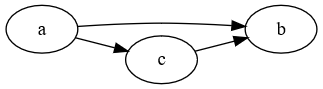
\includegraphics[width=\columnwidth]{abc_dag}
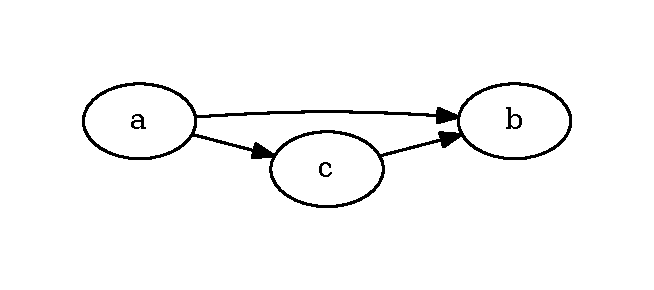
\includegraphics{figures/abc_dag}
%\caption{A directed acyclic graph}
\label{abc_dag}
\end{figure}

Let the basic DFS algorithm begin at vertex $a$. The algorithm marks $a$ explored by adding $a$ to the \texttt{visited} set. The algorithm can continue to $b$, mark $b$ explored, find no out-edge from $b$ and return to $a$. The algorithm then continues to $c$ and finds one out-edge $(c,b)$. Vertex $b$ was already explored but this does not indicate the presence of a cycle.

The simple DFS algorithm can only reliably detect a cycle if the starting vertex $u$ is explored twice. The simple DFS algorithm runs in linear $O(V+E)$ time. One might run DFS $V$ times in $O(V^2+VE)$ to detect if any starting vertex causes a cycle, but there is a better way.

\begin{lstlisting}[columns=fixed,caption={A modified two-color DFS algorithm},label={2colormod}]
static boolean dfs(Map<Integer, List<Integer>> g,
                   int u, Set<Integer> visited,
                   Set<Integer> ancestors) {
  visited.add(u);
  for (int v : g.get(u)) {
    if (visited.contains(v) && ancestors.contains(v)) {
      ancestors.add(v);
      System.out.println("Loop detected: " + ancestors);
      return true;
    } else if (!visited.contains(v)) {
      ancestors.add(v);
      if (dfs(g, v, visited, stack)) return true;
      ancestors.remove(v);
    }
  }
  return false;
}
\end{lstlisting}

The modified two-color algorithm in listing \ref{2colormod} uses its \texttt{ancestor} set to detect back edges. Ultimately, though, a presence of a vertex in either or neither set is no different from a three-color algorithm.

\begin{lstlisting}[columns=fixed,caption={DFS algorithm with three colors},label={3color}]
static enum Color { WHITE, BLACK, GREY };

static boolean dfs(int[][] g, Color[] c, int u) {
  if (g.length == 0 || g.length != c.length ||
      u >= g.length || u < 0)
    throw new IllegalArgumentException();
  c[u] = Color.GREY;
  boolean r = false;
  for (int v : g[u]) {
    switch (c[v]) {
      case WHITE:
      	r |= dfs(g, c, v);
      	break;
      case BLACK: /* skip */
      	break;
      case GREY:  /* loop */
      	r = true;
      	break;
    }
  }
  c[u] = Color.BLACK;
  return r;
}
\end{lstlisting}

The algorithm shown in listing \ref{3color} uses a very different representation for a graph than the previous examples. This algorithm accepts a two-dimensional array representing out-edges. In this array, a value \texttt{v = g[u][i]} denotes an edge $(u,v)$.

\begin{lstlisting}[caption={A two-dimensional array representing the graph shown in figure \ref{redblue}}]
[[]
 [3, 1]
 []
 []
 [2, 6, 8]
 [7, 5, 3]
 [9, 4]
 [6, 4]
 []
 [5, 2, 7, 6]]
 \end{lstlisting}

The color of each vertex is initialized as white. The DFS algorithm marks a node grey when it is first explored and recursively continues to each out-edge. When each out-edge has been explored the vertex has been fully explored and is marked black. If DFS encounters a black vertex no action is necessary. If DFS encounters a grey vertex then the algorithm has detected a cycle.

\begin{figure}
\centering
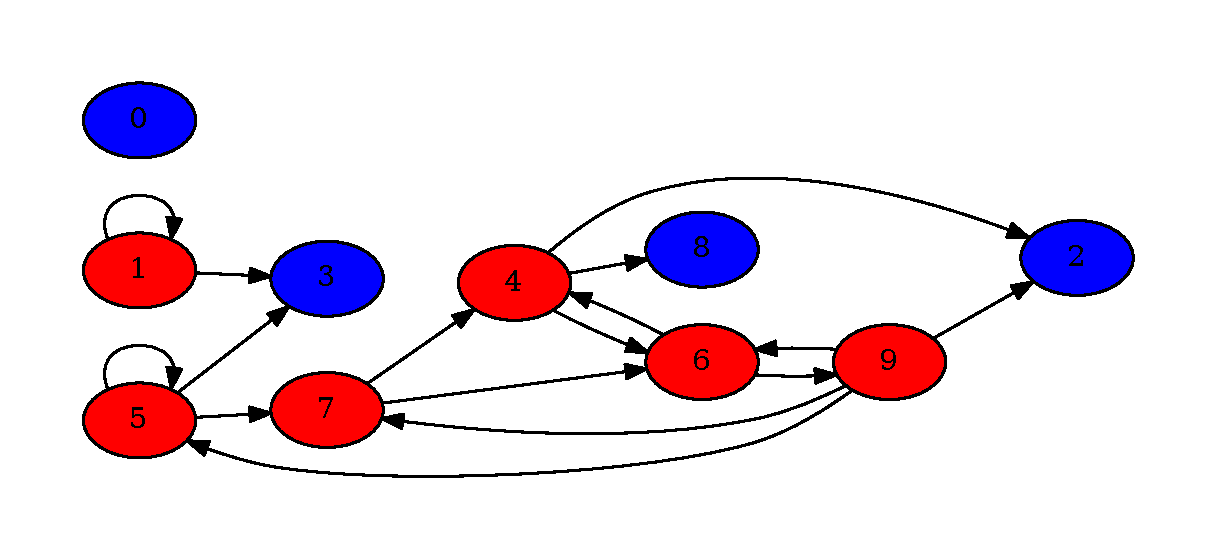
\includegraphics[width=\columnwidth]{figures/redblue}
\caption{Red vertices belong to cyclic components in this directed graph}
\label{redblue}
\end{figure}

DFS explores each vertex exactly once and evaluates each edge exactly once. DFS runs in linear $O(V+E)$ time \cite{cormen2001introduction}.

\chapter{Dynamic Programming}

\section{Fibonacci}

\textit{Dynamic Programming} (DP) has been characterized as an algorithmic technique ``careful brute force'' that combines guessing, recursion, and \textit{memoization} \cite{demaine_dp2}. Dynamic Programming can be used to solve difficult problems where greedy approaches fail.

Recall that the Fibonacci sequence, $F_n=F_{n-1} + F_{n-2}$ with $F_0=0$ and $F_1=1$, can be implemented with a simple recurrence:

\begin{lstlisting}
public static int fibonacci(int n) {
  if (n == 0) return 0;
  else if (n == 1) return 1;
  else return fibonacci(n - 1) + fibonacci(n - 2);
}
\end{lstlisting}

The above algorithm runs in exponential $O(\Phi^n)$ time. A faster DP algorithm makes use of a \textit{dictionary} of $F_k$ terms that can be used to deduplicate subtrees.

\begin{lstlisting}
static int fibonacciDP(int n, Map<Integer, Integer> d) {
  if (!d.containsKey(n)) {
    if (n == 0) d.put(n, 0);
    else if (n == 1) d.put(n, 1);
    else d.put(n, fibonacciDP(n - 1, d) + fibonacciDP(n - 2, d));
  }
  return d.get(n);
}
\end{lstlisting}

The \texttt{fibonacciDP} function accepts a dictionary as an argument. If the dictionary contains value $F_k$ then that value can be immediately returned. Otherwise, the base cases $F_0=0$ and $F_1=1$ are applied or the recursive definition is used to compute $F_k=F_{k-1}+F_{k-2}$. Assuming constant time $O(1)$ addition of fixed-width integers, the \texttt{fibonacciDP} function runs in linear $O(n)$ time. If the dictionary is reused then it acts as a cache for subsequent calls to \texttt{fibonacciDP}. $\texttt{fibonacciDP}(k)$ after $\texttt{fibonacciDP}(n)$ becomes $O(1)$ if $k \le n$ and $O(k - n)$ otherwise.

\section{Height of a Tree}

Memoization in a DP solution does not require an explicit dictionary as above. A binary tree is a collection of nodes containing keys (values) and, optionally, references to left or right children \cite{rhodesTree}. A node with no children has a height of 1. The height of a parent node is one greater than the greater height of each of its children.

\begin{lstlisting}
class Node {
  Node left, right;

  static int height(Node n) {
    if (n == null) return 0;
    else return 1 + Math.max(height(n.left), height(n.right));
  }
}
\end{lstlisting}

The above program provides a general-purpose method for computing the height of any node in a binary tree. All nodes in the tree of size $|V|$ must be visited, hence the ``careful brute force'' description of DP, but there is no need to evaluate or record all $|V|!$ possible permutations. The \texttt{height} function runs in linear $O(|V|)$ time in the worst case.

What happens to this function if the tree contains a loop? That is, what happens if a child of any node is also a parent node to that node? This topology violates the definition of a \textit{tree} (an acyclic graph). The DP approach does not work for cyclic graphs; it must be possible to phrase a problem as a Directed Acyclic Graph (DAG) for DP to be a viable solution.

Special cases of a problem often lead to unique solutions. A left-complete binary tree can be represented in an array of elements $[1..n]$. The left child of any element $i$ is at position $2i$, the right child is at position $2i+1$, and the parent is at $\lfloor n/2 \rfloor$. The height of each node $i$ is given by

\begin{equation*}
\texttt{height}(i) = 1 + \lfloor \log_2{i} \rfloor
\end{equation*}

The special case of a left-complete binary tree, represented in an array instead of a linked list, offers a unique constant time $O(1)$ optimization to compute height.

\section{Paths in a Grid}

Imagine a grid of size $x \times y$. Start at position $(0,0)$ and move either up or right but never left or down. There is only one path to $(1,0)$ (right one) and one path to $(0,1)$ (up one). There are two paths to $(1,1)$ -- right and then up, or up and then right. Positions $(2,0)$, $(0,2)$, and all positions of the forms $(x,0)$ and $(0,y)$ have only one \textit{path} from $(0,0)$. Position $(2,1)$ can be reached by three paths: right, right, up; right, up, right; and up, right, right. 

Analysis quickly reveals that the path count is the sum of those in the left and lower positions:

\begin{lstlisting}
static long paths (int x, int y) {
  if (x == 0 || y == 0) return 1;
  else return p(x-1, y) + p(x, y-1);
}
\end{lstlisting}

Like the simple recursive Fibonacci algorithm, the naive path-counting algorithm is slow. Staggeringly slow. $O({(2n)!}/{(n!)^2})$ slow (see \url{https://oeis.org/A134760}). Memoization to the rescue!

\begin{lstlisting}
static long pathsDP (int x, int y) {
  return pm(x, y, new long[x + 1][y + 1]);
}

private static long pathsDP (int x, int y, long m[][]) {
  if (x == 0 || y == 0) return 1;
  else if (m[x][y] > 0) return m[x][y];
  else return m[x][y] = pathsDP(x - 1, y, m) + pathsDP(x, y - 1, m);
}
\end{lstlisting}

This algorithm has only quadratic $O(n^2)$ complexity (see \url{https://oeis.org/A002061}).

\section{Change Problem}

All of the algorithms shown so far worked ``backwards'' from $n$ to the base case. It is often possible and sometimes necessary to do the opposite.

Making change in as few coins as possible can sometimes be solved using a greedy algorithm \cite{pevznerChange}. For example, if coin denominations are $\{1, 5, 10, 25\}$ then to change 12 cents one subtracts the largest coin less than or equal to the amount and recursively continues until change is made. The algorithm produces optimal solutions for some but not all currencies. Suppose a hypothetical country has coins in $\{1, 4, 6, 10\}$ denominations. The greedy algorithm still changes 12 cents as $\{10,1,1\}$ but this solution is not optimal -- $\{6,6\}$ is better.

A ridiculous brute force solution might be to compute all possible coin combinations that sum to 12 and then select the shortest solution. This would include obviously suboptimal solutions like $\{1,1,1,1,1,1,1,1,1,1,1,1\}$. DP discards useless solutions early and keeps only the optimal solutions at each subproblem.

\begin{lstlisting}
static int changeDP(int D[], int v) {
  if (v < 0) throw new IllegalArgumentException();
  int c[] = new int[v + 1];
  c[0] = 0;
  Arrays.fill(c, 1, v + 1, Integer.MAX_VALUE);
  for (int i = 0 ; i < v ; i++) {
    for (int d : D) {
      if (i + d <= v && c[i] + 1 < c[i + d])
      c[i + d] = c[i] + 1;
    }
  }
  return c[v];
}
\end{lstlisting}

For $D = \{ 1, 4, 6, 10 \}$ and values $v=[0,18]$ this algorithm computes the minimum number of coins as:

\begin{center}
\begin{tabular}{c | c | c | c | c | c | c | c | c | c | c | c | c | c | c | c | c | c | c | c}
$v$ & 0 & 1 & 2 & 3 & 4 & 5 & 6 & 7 & 8 & 9 & 10 & 11 & 12 & 13 & 14 & 15 & 16 & 17 & 18 \\
\hline
$\texttt{changeDP}(v)$ & 0 & 1 & 2 & 3 & 1 & 2 & 1 & 2 & 2 & 3 & 1 & 2 & 2 & 3 & 2 & 3 & 2 & 3 & 3
\end{tabular}
\end{center}

This algorithm run in $O(|D| \times v)$ time --- polynomial, but disappointingly complex for large $v$. If the values of $D$ are sparse then it is possible to use a memoized recursive definition, much like \texttt{fibonacciDP}:

\begin{lstlisting}
static int changeDP(int D[], int v, Map<Integer, Integer> c) {
  if (v < 0) throw new IllegalArgumentException();
  else if (v == 0) return 0;

  int m = Integer.MAX_VALUE;
  for (int d : D) {
    if (v >= d)
      m = Math.min(m, 1 + change(D, v - d, c));
  }
  c.put(v, m);

  return m;
}
\end{lstlisting}

Notice that the modified \texttt{changeDP} function has no advantage if $1 \in D$. Suppose $D = \{ 2 \}$, then the dictionary will be populated with all values $c_i$ where $2 | i$. The total work is only $O(\frac{1}{2} v) = O(\frac{1}{2} |D| \times v) = O(|D| \times v)$ --- the asymptotic complexity remains unchanged. In practice, the recursive variant may be slower by some constant factor due to stack framing. 

\section{Longest Common Subsequence}

Given two sequences $A = (a_1, a_2, ... , a_n)$ and $B = (b_1, b_2, ... , b_m)$, the Longest Common Subsequence (LCS) is the largest subsequence where $(a_{i_1} = b_{j_1} , ... , a_{i_p} = b_{j_p})$. LCS algorithms is useful in text comparison, such as the \texttt{diff} program, and has applications to bioinformatics.

It is possible to enumerate all $2^n$ possible subsequences of $A$ and $B$, then compare each combination and find the longest, but this algorithm would run in exponential $O(2^n)$ time.

A well-known DP algorithm to find the LCS constructs an two dimensional array $c$ of size $(n+1) \times (m+1)$. All positions along the top and left are initialized to $c[0][j] = c[i][0] = 0$. The algorithm then iterates through all positions $c[i][j]$ and sets $c[i][j] = c[i+1][j+1] + 1$ if $A_i = B_j$ and the maximum of $c[i-1][j]$ and $c[i][j-1]$ otherwise. The value at position $c[n + 1][m + 1]$ contains the length of the LCS when the outer loop completes. The algorithm runs in polynomial $O(n \times m)$ time.

\begin{lstlisting}
static int lcs(char A[], char B[]) {
  int c[][] = new int[A.length + 1][B.length + 1];
  for (int i = 1 ; i <= A.length ; i++) {
    for (int j = 1 ; j <= B.length ; j++) {
      if (A[i-1] == B[j-1]) c[i][j] = c[i-1][j-1] + 1;
      else c[i][j] = Math.max(c[i-1][j], c[i][j-1]);
    }
  }
  return c[A.length][B.length];
}
\end{lstlisting}

The $c$ array generated from the strings ``mello'' and ``yellow'' are shown below:

\begin{center}
\begin{tabular}{c | c | c | c | c | c | c | c }
& & y & e & l & l & o & w \\
\hline
 & 0 & 0 & 0 & 0 & 0 & 0 & 0 \\
\hline
m & 0 & 0 & 0 & 0 & 0 & 0 & 0 \\
\hline
e & 0 & 0 & 1 & 1 & 1 & 1 & 1 \\
\hline
l & 0 & 0 & 1 & 2 & 2 & 2 & 2 \\
\hline
l & 0 & 0 & 1 & 2 & 3 & 3 & 3 \\
\hline
o & 0 & 0 & 1 & 2 & 3 & 4 & 4
\end{tabular}
\end{center}

\section{Partition Problem}

This last DP algorithm has an important property that differentiates it from those described so far: subproblems overlap. Given a sequence or real numbers $A = (a_1, a_2, ... , a_n)$, divide the sequence into three partitions such that sum of each partition is equal.

Some sequences obviously have no solution. $(1,1,1,1)$ has a sum of 4 and $3 \not | 4$ so no solution can exist. $(3,3,3,3)$ has a sum of 12 and $3 | 12$, but it is immediately obvious at a glance that no solution exists. The sequence $(62,88,36,8,33,25,12,76,24,38,51)$ is short but not at all obvious.

This problem is known to be NP-complete. No known algorithm can solve the partition problem in polynomial time and it is widely hypothesized that no such algorithm exists.

A DP algorithm to compute whether a solution exists has to consider the impact of adding an element to each of the three partitions separately, recursively considering each possibility until a solution is discovered or no solutions exist.

\begin{lstlisting}
static boolean part3(int a[]) {
  List<Integer> A = new LinkedList<>();
  for (int i : a)
    A.add(i);
  return dfs(A, 0, 0, 0);
}

private static boolean dfs(List<Integer> A, int x, int y, int z) {
  if (A.isEmpty())
    return (x == y && y == z);
  int v = A.remove(0);
  boolean r = dfs(A, x + v, y, z) ||
    dfs(A, x, y + v, z) || dfs(A, x, y, z + v);
  A.add(0, v);
  return r;
}
\end{lstlisting}

The use of the \texttt{||} short-circuit operator allows the algorithm to halt immediately if a solution exists.

\chapter{Finite-State Machines}

\chapter{2D Graphics}

The standard form of a linear equation takes the form $Ax+By=C$. Given two equations

\begin{equation*}5x-3y=10\end{equation*}
\begin{equation*}2x+8y=32\end{equation*}

We can combine these equations with simple addition, rearrange, and factor to produce.

\begin{equation*}5x-3y + 2x+8y = 10 + 32\end{equation*}
\begin{equation*}5x + 2x+8y -3y= 10 + 32\end{equation*}
\begin{equation*}(5 + 2)x + (8 -3)y= 10 + 32\end{equation*}

The coefficients can be represented in a matrix.

\begin{equation*}
\begin{bmatrix}
5 & -3 \\
2 & 8
\end{bmatrix} \times 
\begin{bmatrix}x \\ y\end{bmatrix} = 
\begin{bmatrix}10 \\ 32\end{bmatrix}
\end{equation*}

A matrix is rectangular array of values with many useful properties. Matrices were originally developed for solving linear equations in many dimensions. Just as numbers can be applied to many purposes, so can matrices.

One common use of a matrix is to represent a vector. A vector is a quantity with direction and magnitude but not position. The notation $\vec{v}=(x,y)$ can be used to represent a vector rooted at $(0,0)$ pointing towards $(x,y)$ with a magnitude of $\lvert\vec{v}\rvert=\sqrt{x^2 + y^2}$. A unit vector has a magnitude of 1.

Converting an angle $\Theta$ to a unit vector $\vec{v}$ is simple: $\vec{v}=(\cos{\Theta},\sin{\Theta})$. All vectors of the form $(k x, k y)$ (where $k \ne 0$) are parallel to $(x,y)$.

Matrix addition is straightforward. Given $m \times n$ matrices $A$ and $B$, $A+B$ is computed by adding each element to that in the corresponding position. Matrices can only be added if they have the same numbers of rows and columns. The row-major notation $M_{ij}$ is used to refer to a single element in a matrix. Starting from $M_{11}$ at the top-left corner, $i$ represents the horizontal row and $j$ represents the vertical column.

\begin{equation}
\begin{split}
A+B
&
=
\begin{bmatrix}
A_{11} & A_{12} & \cdots & A_{1n} \\
A_{21} & A_{22} & \cdots & A_{2n} \\
\vdots & \vdots & \ddots & \vdots \\
A_{m1} & A_{m2} & \cdots & A_{mn} \\
\end{bmatrix} +
\begin{bmatrix}
B_{11} & B_{12} & \cdots & B_{1n} \\
B_{21} & B_{22} & \cdots & B_{2n} \\
\vdots & \vdots & \ddots & \vdots \\
B_{m1} & B_{m2} & \cdots & B_{mn} \\
\end{bmatrix} \\
&
=
\begin{bmatrix}
A_{11} + B_{11} & A_{12} + B_{12} & \cdots & A_{1n} + B_{1n} \\
A_{21} + B_{21} & A_{22} + B_{22} & \cdots & B_{2n} + B_{2n} \\
\vdots & \vdots & \ddots & \vdots \\
A_{m1} + B_{m1} & B_{m2} + B_{m2} & \cdots & A_{2n} + B_{mn} \\
\end{bmatrix}
\end{split}
\end{equation}

Matrix multiplication is much less obvious. Several forms of matrix multiplication have been developed. The cross product multiplies matrices of size $m \times k$ and $k \times n$ and produces a new matrix of size $m \times n$. Each position $M_{ij}$ is equal to the sum of each product $A_{ik}B_{hk}$ in multiplicands $A$ and $B$.

\begin{equation}
\begin{split}
A \times B
&
=
\begin{bmatrix}
A_{11} & \cdots & A_{1k} \\
A_{21} & \cdots & A_{2k} \\
\vdots & \ddots & \vdots \\
A_{m1} & \cdots & A_{mk} \\
\end{bmatrix} \times
\begin{bmatrix}
B_{11} & B_{12} & \cdots & B_{1n} \\
\vdots & \vdots & \ddots & \vdots \\
B_{k1} & B_{k2} & \cdots & B_{kn} \\
\end{bmatrix} \\
&
=
\begin{bmatrix}
A_{11} B_{11} + A_{12}B_{21} + \cdots + A_{1k}B_{k1} & 
\cdots &
A_{11} B_{1n} + A_{12}B_{2n} + \cdots + A_{1k}B_{kn} \\
\vdots & \ddots & \vdots \\
A_{m1} B_{11} + A_{m2}B_{21} + \cdots + A_{mk}B_{k1} & 
\cdots &
A_{m1} B_{1n} + A_{m2}B_{2n} + \cdots + A_{mk}B_{kn}
\end{bmatrix}
\end{split}
\end{equation}

Matrix multiplication may appear quite strange but it is very useful. Vectors can be represented as column matrices.

\begin{equation*}
\vec{v} = (x,y) = \begin{bmatrix}x \\ y\end{bmatrix}
\end{equation*}

Multiplying $\vec{v}$ by the $2 \times 2$ identity matrix $I_2$ makes no change.
\begin{equation*}I_2 \times \vec{v} =
\begin{bmatrix}1 & 0 \\ 0 & 1\end{bmatrix} \times 
\begin{bmatrix}x \\ y\end{bmatrix} = \begin{bmatrix}x \\ y\end{bmatrix}
\end{equation*}

Note that because the cross product only exists for matrices of $m \times k$ and $k \times n$ it is not possible to compute $\vec{v} \times I_2$. The cross product is not commutative. The matrix product is, however, associative.

\begin{equation}\label{associative}
(M_2 \times M_1) \times \vec{v} = M_2 \times (M_1 \times \vec{v})
\end{equation}

One application for repeatedly applying cross products to vectors is for linear transformations, such as to compute movement in a video game.

Suppose a vectors $\vec{v_1}=(0,0)$, $\vec{v_2}=(100,0)$, $\vec{v_3}=(100,100)$, and $\vec{v_4}=(0,100)$ are used to represent the four corners of a square in a game. The developer needs to stretch the box into a rectangle of twice the width and half the height. It is obvious that the developer need only half the $y$ value and double the $x$ coordinate for each vector. This can be accomplished with a cross product by:

\begin{equation*}\begin{bmatrix}2 & 0 \\ 0 & 1/2\end{bmatrix} \times \begin{bmatrix}x \\ y\end{bmatrix} = \begin{bmatrix}2x \\ y/2\end{bmatrix}\end{equation*}

In general, a vector can be scaled by a factor of $a$ in $x$ and by a factor of $b$ in $y$ using the following transformation matrix:

\begin{equation}\label{scale}
S_{a,b}=\begin{bmatrix}a & 0 \\ 0 & b\end{bmatrix}\end{equation}

Rotations are more tricky. Suppose $\vec{v} = (k \cos{\alpha}, k \sin{\alpha}) = k \cdot (\cos{\alpha}, \sin{\alpha})$. For now, assume $k=1$ (it will not matter later). We want a transformation matrix $M_{\beta}$ that produces

\begin{equation*}M_{\beta} \times \begin{bmatrix}\cos{\alpha} \\ \sin{\alpha}\end{bmatrix} = \begin{bmatrix}\cos{\alpha + \beta} \\ \sin{\alpha + \beta}\end{bmatrix}\end{equation*}

For this we use Ptolemy's Sum and Difference Formulae:

\begin{equation*}
\cos{\alpha \pm \beta} = \cos{\alpha}\cos{\beta} \mp \sin{\alpha}\sin{\beta}
\end{equation*}
\begin{equation*}
\sin{\alpha \pm \beta} = \cos{\alpha}\sin{\beta} \pm \sin{\alpha}\cos{\beta}
\end{equation*}

Substitute these identities into the equation involving $M_\beta$ to find

\begin{equation*}M_{\beta} \times \begin{bmatrix}\cos{\alpha} \\ \sin{\alpha}\end{bmatrix} = \begin{bmatrix}\cos{\alpha}\cos{\beta} - \sin{\alpha}\sin{\beta} \\ \cos{\alpha}\sin{\beta} + \sin{\alpha}\cos{\beta}\end{bmatrix}\end{equation*}

It is now possible to recognize a $2 \times 2$ matrix that produces the desired cross product.

\begin{equation*}
\begin{bmatrix}\cos{\beta} & - \sin{\beta} \\ \sin{\beta} & \cos{\beta}\end{bmatrix}
\times \begin{bmatrix}\cos{\alpha} \\ \sin{\alpha}\end{bmatrix} = \begin{bmatrix}\cos{\alpha}\cos{\beta} - \sin{\alpha}\sin{\beta} \\ \cos{\alpha}\sin{\beta} + \sin{\alpha}\cos{\beta}\end{bmatrix}\end{equation*}

Notice that it is possible to reintroduce constant multipliers $k$ that were previously discarded using the dot product.

\begin{equation*}k \cdot \begin{bmatrix}\cos{\alpha}\cos{\beta} - \sin{\alpha}\sin{\beta} \\ \cos{\alpha}\sin{\beta} + \sin{\alpha}\cos{\beta}\end{bmatrix} = \begin{bmatrix}k ( \cos{\alpha}\cos{\beta} - \sin{\alpha}\sin{\beta} ) \\ k (\cos{\alpha}\sin{\beta} + \sin{\alpha}\cos{\beta})\end{bmatrix}\end{equation*}

The generalized transformation matrix to rotate a vector around angle $\Theta$ is:

\begin{equation}\label{rotation}
R_\Theta = \begin{bmatrix}\cos{\Theta} & -\sin{\Theta} \\ \sin{\Theta} & \cos{\Theta}\end{bmatrix}
\end{equation}

Finally, we want to translate a vector. This may sound strange, since a vector is a quantity without position, but it is possible to fake it by adding an additional dimension. Yes, it's weird. Yes, 3D graphics do require 4D math.

Return to the squished rectangle represented by vectors $\vec{v_1}$, $\vec{v_2}$, $\vec{v_3}$, and $\vec{v_4}$. To move each of the four coordinates up by 100 units it might be obvious to simply add 100 to the $y$ coordinate. Why bother searching for a solution involving cross products?

The motivation lies in equation \ref{associative}: cross products may be chained to apply transformations in an object's local coordinate system. In other words, it is possible to rotate an object and then move it ``up'' from the object's new perspective. This is the power and beauty of the transformation matrices presented here.

Add an unused dimension $w$ to an identity matrix and use the right column to translate each dimension. The value $w=1$ should be inferred for each vector. To translate $\vec{v_2}=(200,50)$ up by 100 units:

\begin{equation*}
\begin{bmatrix}1 & 0 & 0 \\ 0 & 1 & 100 \\ 0 & 0 & 1 \end{bmatrix} \times
\begin{bmatrix}200 \\ 50 \\ 1\end{bmatrix} = 
\begin{bmatrix}200 \\ 150 \\ 1\end{bmatrix}
\end{equation*}

Performing scales and rotations in two-dimensions but against a three-dimensional vector (where $w=1$) requires a minor update to the translation matrices shown in equations \ref{scale} and \ref{rotation}. Together, the three transformation matrices are:

\begin{equation}\label{eq:scale2}
S_{a,b}=\begin{bmatrix}a & 0 & 0\\ 0 & b & 0\\ 0 & 0 & 1\end{bmatrix}
\end{equation}
\begin{equation}\label{eq:rotate2}
R_\Theta = \begin{bmatrix}\cos{\Theta} & -\sin{\Theta} & 0\\ \sin{\Theta} & \cos{\Theta} & 0 \\ 0 & 0 & 1\end{bmatrix}
\end{equation}
\begin{equation}\label{eq:translate2}
T_{a,b}=\begin{bmatrix}1 & 0 & a\\0 & 1 & b\\0 & 0 & 1\end{bmatrix}
\end{equation}

Observe that the bottom row of each transformation consists of a series of zeros and ends with a one -- just like an identity matrix. The cross product between two square matrices sharing an identity row will produce a matrix with the same identity row.

\begin{equation*}
\begin{bmatrix}a & b & c \\ d & e & f \\ 0 & 0 & 1\end{bmatrix} \times
\begin{bmatrix}g & h & i \\ j & k & l \\ 0 & 0 & 1\end{bmatrix} = 
\begin{bmatrix}ag + bj & ah + bk & ai + bi \\
dg + ej & dh + ek & di + el \\
0 & 0 & 1
\end{bmatrix}
\end{equation*}

Transformation matrices can be chained, but because cross multiplication is not commutative the order of operations matters.

Take a vector $\vec{v}=(1,0)$ parallel to the $x$-axis with a magnitude of 1 and placeholder dimension $w=1$. Now, apply $T_{1,0}$ and $R_{\pi/2}$.

\begin{equation*}
T_{1,0} \times R_{\pi/2} \times \vec{v} = 
\begin{bmatrix}1 & 0 & 1 \\ 0 & 1 & 0 \\ 0 & 0 & 1\end{bmatrix} \times
\begin{bmatrix}0 & -1 & 0 \\ 1 & 0 & 0 \\ 0 & 0 & 1\end{bmatrix} \times
\begin{bmatrix}1 \\ 0 \\ 1\end{bmatrix} = 
\begin{bmatrix}0 & -1 & 1 \\ 1 & 0 & 0 \\ 0 & 0 & 1\end{bmatrix} \times
\begin{bmatrix}1 \\ 0 \\ 1\end{bmatrix} =
\begin{bmatrix}1 \\ 1 \\ 1\end{bmatrix}
\end{equation*}

\begin{equation*}
R_{\pi/2} \times T_{1,0} \times \vec{v} = 
\begin{bmatrix}0 & -1 & 0 \\ 1 & 0 & 0 \\ 0 & 0 & 1\end{bmatrix} \times
\begin{bmatrix}1 & 0 & 1 \\ 0 & 1 & 0 \\ 0 & 0 & 1\end{bmatrix} \times
\begin{bmatrix}1 \\ 0 \\ 1\end{bmatrix} = 
\begin{bmatrix}0 & -1 & 0 \\ 1 & 0 & 1 \\ 0 & 0 & 1\end{bmatrix} \times
\begin{bmatrix}1 \\ 0 \\ 1\end{bmatrix} =
\begin{bmatrix}0 \\ 2 \\ 1\end{bmatrix}
\end{equation*}

$T_{1,0} \times R_{\pi/2} \times \vec{v}$ rotates $\vec{v}$ to a become parallel to the $y$-axis and then translates the vector one unit to the right. $R_{\pi/2} \times T_{1,0} \times \vec{v}$ performs operations in the opposite sequence to a different effect. $\vec{v}$ is translated to $(2,0)$ and is then rotated to $(0,2)$. Transformations applied to the left occurs in global coordinate space. Transformations applied to the right occurs in the object's local coordinate space.

Cascading Style Sheets (CSS) allow elements to be translated, rotated, and scaled using transformations (\url{https://drafts.csswg.org/css-transforms/}). These transformations are provided to CSS through functions instead of strings. For example, 

\begin{lstlisting}
<div style="transform: matrix(a, b, c, d, e, f);">
Hello world!
</div>
\end{lstlisting}

The \texttt{matrix} function is shorthand for a transformation in two dimensions of the following form. CSS also supports three-dimensional transformations using the \texttt{matrix3d} function with 16 numeric parameters describing a transformation matrix in column-major order.

\begin{equation*}
M = \begin{bmatrix}a & c & 0 & e\\b & d & 0 & f\\0 & 0 & 1 & 0\\0 & 0 & 0 & 1\end{bmatrix}
\end{equation*}

The following HTML program contains buttons that translate an element using its own trivial cross product function. The same program is posted at \url{https://wjholden.com/2d.html}. Try it out!

\begin{lstlisting}
<!doctype html>
<html>
<head>
<meta charset="UTF-8">
<title>2D Transforms in CSS</title>
<script>
var transform = [ 1, 0, 0, 0, 1, 0, 0, 0, 1];
    
function crossProduct3x3(m1, m2) {
    // this function only works for two 3x3 square matrices
    var p = new Array(9);
    p[0] = m1[0] * m2[0] + m1[1] * m2[3] + m1[2] * m2[6];
    p[1] = m1[0] * m2[1] + m1[1] * m2[4] + m1[2] * m2[7];
    p[2] = m1[0] * m2[2] + m1[1] * m2[5] + m1[2] * m2[8];

    p[3] = m1[3] * m2[0] + m1[4] * m2[3] + m1[5] * m2[6];
    p[4] = m1[3] * m2[1] + m1[4] * m2[4] + m1[5] * m2[7];
    p[5] = m1[3] * m2[2] + m1[4] * m2[5] + m1[5] * m2[8];

    p[6] = m1[6] * m2[0] + m1[7] * m2[3] + m1[8] * m2[6];
    p[7] = m1[6] * m2[1] + m1[7] * m2[4] + m1[8] * m2[7];
    p[8] = m1[6] * m2[2] + m1[7] * m2[5] + m1[8] * m2[8];
    return p;
}

function formatMatrix(m) {
    // assume m is an array representing a row-major 3x3 matrix
    return "matrix(" + m[0] + "," + m[3] + "," + m[1] + "," +
            m[4] + "," + m[2] + "," + m[5] + ")";
}

function updateScreen(m, global) {
    if (global) {
        transform = crossProduct3x3(m, transform);
    } else {
        transform = crossProduct3x3(transform, m);
    }
    document.getElementById("hello").style.transform =
            formatMatrix(transform);
    var s = transform.slice(0, 3).toString() + "\n" +
            transform.slice(3, 6).toString() + "\n" +
            transform.slice(6, 9).toString();
    document.getElementById("matrix").value = s;
}
</script>
</head>

<body onload="updateScreen(transform, false);">

<table>
<tr>
<td>Global Transforms: </td>
<td><input type="button" value="&larr;"
        onclick="updateScreen([1,0,-10,0,1,0,0,0,1], true);"></td>
<td><input type="button" value="&rarr;"
        onclick="updateScreen([1,0,10,0,1,0,0,0,1], true);"></td>
<td><input type="button" value="&uarr;"
        onclick="updateScreen([1,0,0,0,1,-10,0,0,1], true);"></td>
<td><input type="button" value="&darr;"
        onclick="updateScreen([1,0,0,0,1,10,0,0,1], true);"></td>        
<td><input type="button" value="&#8634;"
        onclick="updateScreen(
                    [Math.cos(-Math.PI/9),-Math.sin(-Math.PI/9),0,
                    Math.sin(-Math.PI/9),Math.cos(-Math.PI/9),0,
                    0,0,1], true);"></td>
<td><input type="button" value="&#8635;"
        onclick="updateScreen(
                    [Math.cos(Math.PI/9),-Math.sin(Math.PI/9),0,
                    Math.sin(Math.PI/9),Math.cos(Math.PI/9),0,
                    0,0,1], true);"></td>
<td><input type="button" value="&frac23;&times;"
        onclick="updateScreen([2/3,0,0,0,2/3,0,0,0,1], true);"></td>
<td><input type="button" value="1.5&times;"
        onclick="updateScreen([3/2,0,0,0,3/2,0,0,0,1], true);"></td>
<td><input type="button" value="Reset"
        onclick="transform = [1,0,0,0,1,0,0,0,1];
                    updateScreen(transform, false);"></td>
</tr>
<tr>
<td>Local Transforms: </td>
<td><input type="button" value="&larr;"
        onclick="updateScreen([1,0,-10,0,1,0,0,0,1], false);"></td>
<td><input type="button" value="&rarr;"
        onclick="updateScreen([1,0,10,0,1,0,0,0,1], false);"></td>
<td><input type="button" value="&uarr;"
        onclick="updateScreen([1,0,0,0,1,-10,0,0,1], false);"></td>
<td><input type="button" value="&darr;"
        onclick="updateScreen([1,0,0,0,1,10,0,0,1], false);"></td>        
<td><input type="button" value="&#8634;"
        onclick="updateScreen(
                    [Math.cos(-Math.PI/9),-Math.sin(-Math.PI/9),0,
                    Math.sin(-Math.PI/9),Math.cos(-Math.PI/9),0,
                    0,0,1], false);"></td>
<td><input type="button" value="&#8635;"
        onclick="updateScreen(
                    [Math.cos(Math.PI/9),-Math.sin(Math.PI/9),0,
                    Math.sin(Math.PI/9),Math.cos(Math.PI/9),0,
                    0,0,1], false);"></td>
<td><input type="button" value="&frac23;&times;"
        onclick="updateScreen([2/3,0,0,0,2/3,0,0,0,1], false);"></td>
<td><input type="button" value="1.5&times;"
        onclick="updateScreen([3/2,0,0,0,3/2,0,0,0,1], false);"></td>
<td></td>
</tr>
</table>

<textarea id="matrix" rows="3" cols="80"></textarea>
    
<div id="hello" style="width: 100px; text-align: center;">
Hello World!
</div>

</body>
</html>
\end{lstlisting}

\chapter{Multicasting Datagrams}

Computers are networked using many layered communication protocols. The Open Systems Interconnection (OSI) model is commonly referenced to loosely model these protocols. The lowest level, level one, is the physical layer where cables and antennas transmit and receive decibels of power. Layer two is known as the data-link layer. This is the lowest level where communicating devices are uniquely assigned addresses. Devices on the same local area network use layer two addresses to communicate directly. Layer three, the network layer, also provides unique addressing for devices but is used to signal distant devices across wide area networks. The forth layer, the session layer, abstracts a communicating device into many ports. Ports address applications and processes running on the device.

\begin{center}
\begin{tabular}{c | c | c | c | c}
Layer & Name & PDU & Implementation & Address \\
\hline
4 & Session & Segment & TCP and UDP & Port \\
3 & Network & Packet & IP & IP Address \\
2 & Data-Link & Frame & Ethernet and WiFi & MAC Address \\
\end{tabular}
\end{center}

The Internet Protocol is a best-effort and connectionless protocol that forwards packets by destination address using a distributed control plane. This means:

\begin{itemize}
\item IP provides no built-in mechanism to retransmit lost or corrupt packets.
\item IP requires no call setup or resource reservation.
\item IP provides no bandwidth or delay guarantees, nor does IP provide flow control features to limit path saturation.
\item IP does not guarantee that packets will be delivered in the sequence that they were sent.
\item IP routers make autonomous forwarding decisions using connected routes, static routes, and routes learned using a dynamic routing protocol. IP routers are not centrally controlled.
\end{itemize}

X.25 and ATM provide many features that IP does not. IP does not provide these features because these features are not beneficial for every application.

\begin{lstlisting}
function Tx-Syslog {
  Param(
    [Parameter(Mandatory=$true, ParameterSetName="IP Address")]
    [string]$IPAddress,

    [Parameter(Mandatory=$true)]
    [string]$Message
  )

  $ep = New-Object IPEndPoint (
  [IPAddress]::Parse($IPAddress), 514);
  try
  {
    $socket = New-Object System.Net.Sockets.UdpClient;
    $socket.Connect($ep);
    $bytes = [System.Text.Encoding]::ASCII.GetBytes($message);
    $i = $socket.Send($bytes, $bytes.length);
  }
  catch [System.Net.Sockets.SocketException]
  {
    Write-Error "Unable to send Syslog message to $IPAddress";
  }
  finally
  {
    $socket.Close();
  }
}
\end{lstlisting}

\begin{lstlisting}
function Rx-Syslog {
  Param(
    [Parameter(Mandatory=$true, ParameterSetName="IP Address")]
    [string]$IPAddress
  )

  $ep = New-Object IPEndPoint ([IPAddress]::Any, 0);

  try
  {
    $socket = New-Object System.Net.Sockets.UdpClient 514;
    $socket.JoinMulticastGroup(([IPAddress]::Parse($IPAddress)));
    $bytes = $socket.Receive([ref] $ep);
    [System.Text.Encoding]::ASCII.GetString($bytes); 
  }
  catch [System.Net.Sockets.SocketException]
  {
    Write-Error "Unable to receive Syslog messages on $IPAddress";
  }
  finally
  {
    $socket.Close();
  }
}
\end{lstlisting}

\chapter{Attractors}

\section{Kaprekar}

Take any integer $1000 \le x < 10000$. Sort the digits of $x$ in descending and ascending order, padding with zeros as needed. Subtract the sorted digits and assign the difference to $x$. For example, starting with $x = 1005$:

\begin{align*}
5100 - 0015 &= 5085\\
8550 - 0558 &= 7992\\
9972 - 2799 &= 7173\\
7731 - 1377 &= 6354\\
6543 - 3456 &= 3087\\
8730 - 0378 &= 8352\\
8532 - 2358 &= 6174\\
7641 - 1467 &= 6174
\end{align*}

The algorithm cycles at 6174! The integer 6174 is named Kaprekar's Constant \cite{seligman_6174}. Using the ``sort and subtract'' algorithm described, all four-digit integers, with at least two different digits, lead to 6174. (Degenerate cases 1111, 2222, 3333, etc attract to 0000). This cycle is an example of an attractor. An attractor is a fixed point (like 6174) or finite set of points that produce a cycle in a deterministic sequence. Figure \ref{kaprekarTree} shows a graph of integers attracting to 6174 and listing \ref{kaprekarCode} shows a program to compute these sequences.

For relatively small input sets, such as the 8999 integers between 1000 and 10000, one does not need high mathematics to prove or disprove the existence of an attractor. One simply needs a fast computer, patience, or both. Even seemingly large input spaces, such as the $2^{32} = 4294967296$ integers representable by a 32-bit ``double-word,'' can be tested exhaustively for attractors through brute force.

\begin{figure}[H]
\centering
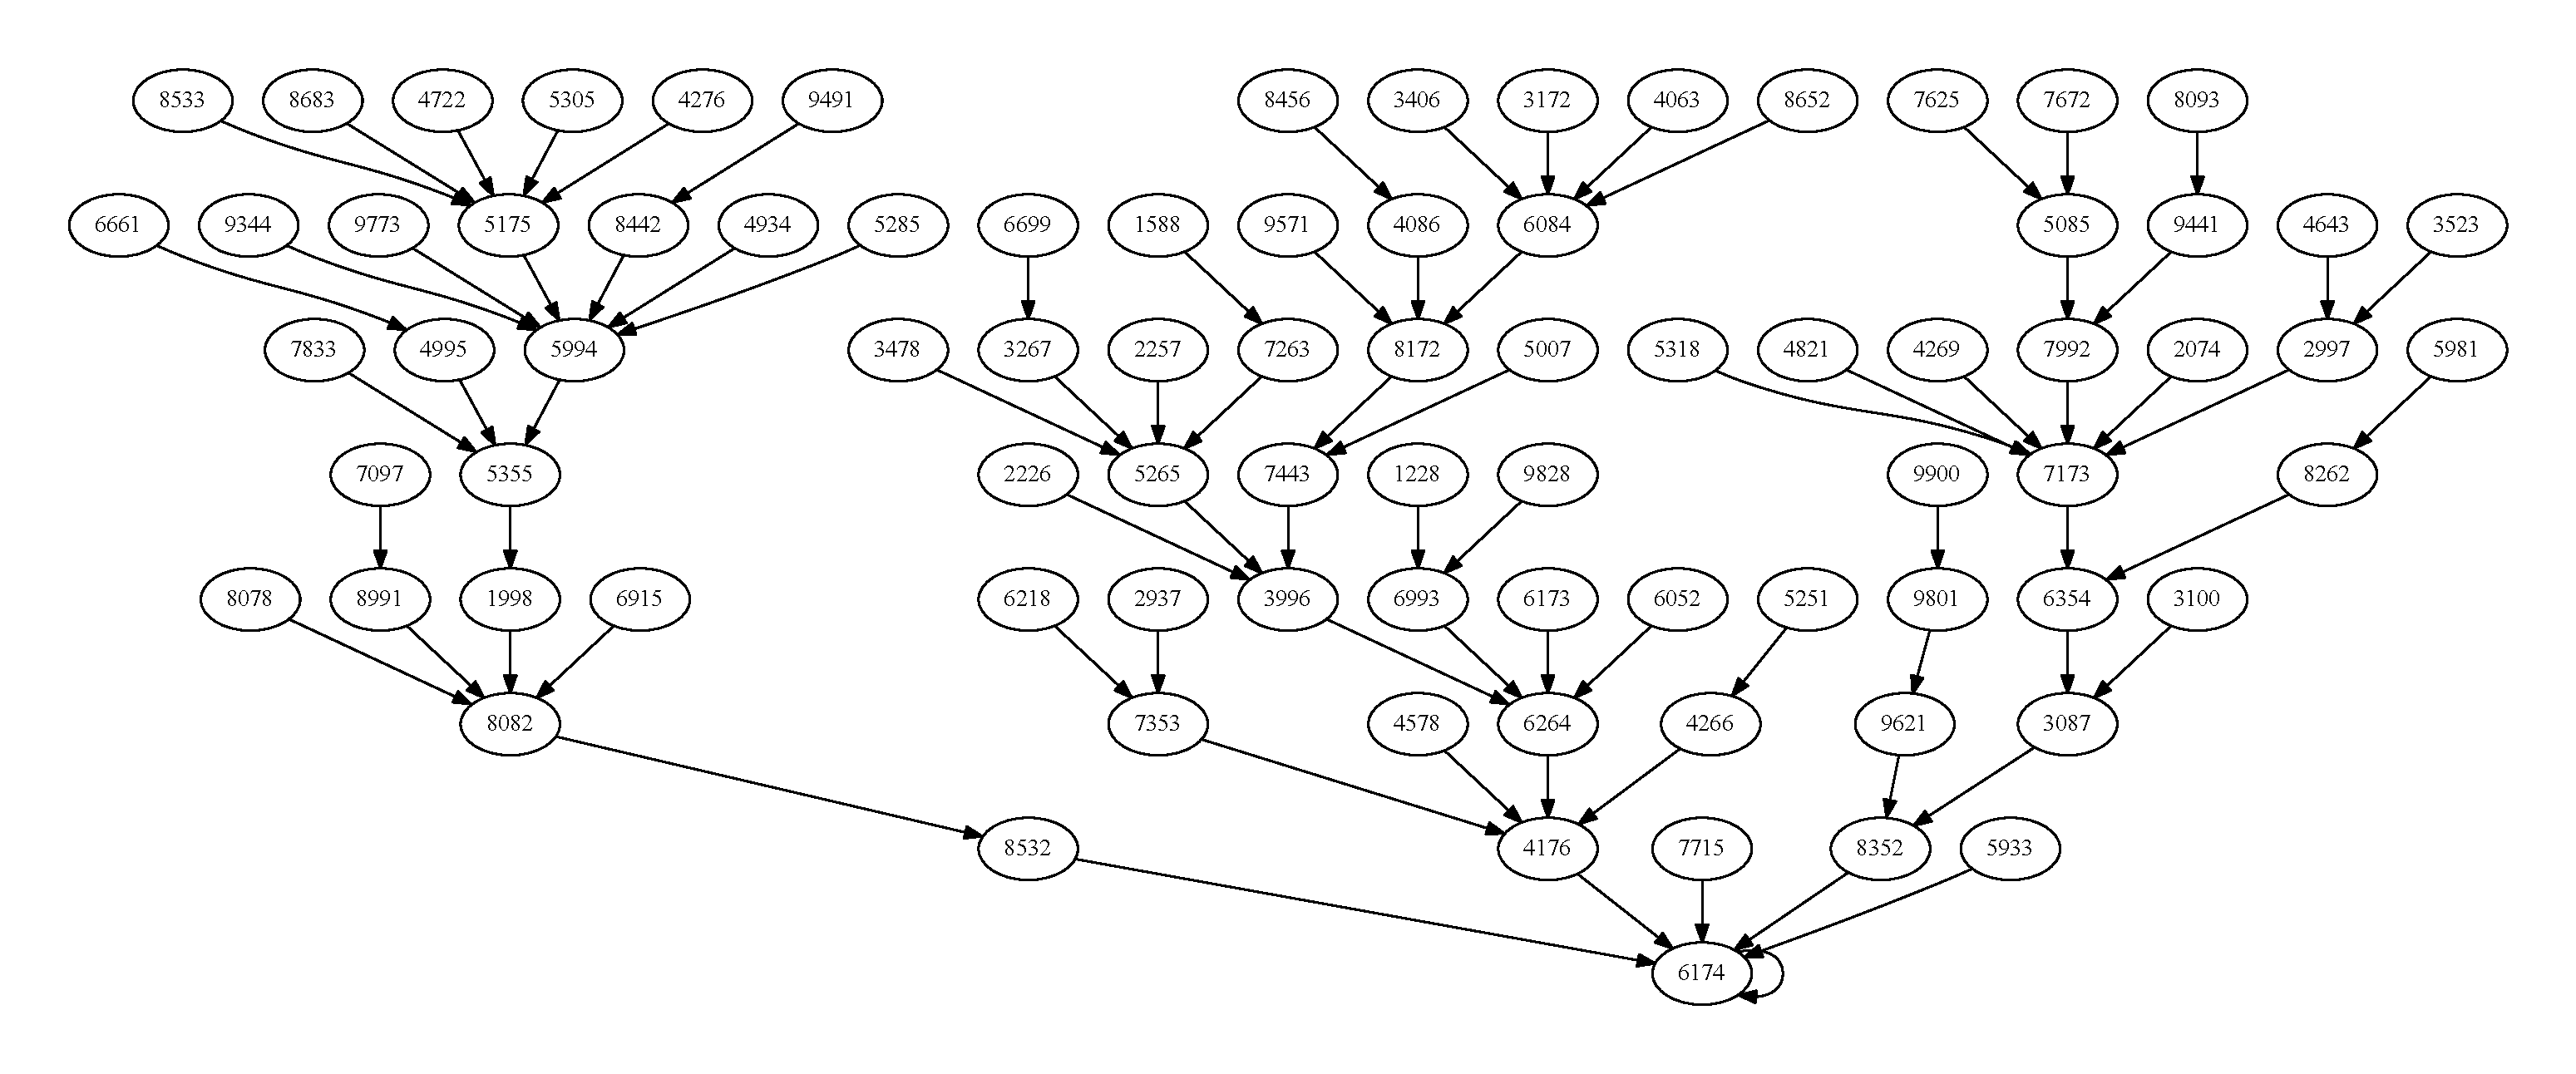
\includegraphics[width=\columnwidth]{figures/kaprekar}
\caption{A sample of four-digit numbers all lead to Kaprekar's Constant}
\label{kaprekarTree}
\end{figure}

\begin{lstlisting}[caption={A program to compute Kaprekar four-digit sequences},label={kaprekarCode}]
import java.util.Arrays;

public class Kaprekar {    
  public static int next(int i, int radix, int length) {
    int a[] = toArray(i, radix, length);
    int b[] = toArray(i, radix, length);
    Arrays.sort(a);
    Arrays.sort(b);
    reverse(a);
    int c[] = subtract(a, b, radix);
    return toInteger(c, radix);
  }

  private static int[] toArray(int i, int radix, int length) {
    int a[] = new int[length];
    for (int k = 0 ; k < length ; k++) {
      a[k] = (int) ((i / Math.pow(radix, length - k - 1)) % radix);
    }
    return a;
  }

  private static int toInteger(int a[], int radix) {
    int i = 0;
    for (int d : a) {
      i = (i * radix) + d;
    }
    return i;
  }

  private static int[] subtract(int a[], int b[], int radix) {
    int i;
    int j = toInteger(a, radix);
    int k = toInteger(b, radix);
    i = Math.abs(j - k);
    return toArray(i, radix, a.length);
  }

  private static void reverse(int a[]) {
    for (int i = 0 ; i < a.length / 2 ; i++) {
      int tmp = a[i];
      a[i] = a[a.length - i - 1];
      a[a.length - i - 1] = tmp;
    }
  }
}
\end{lstlisting}

\section{Pseudorandom Number Generators}

A pseudorandom number generator (PRNG) is a security-critical application that should be evaluated for attractors. A computer program generally accepts input, processes the output using an algorithm, and produces some output. Computer hardware and software should always produce identical results given identical input. This model makes producing a software-only random number generator challenging.

A true random number generator (TRNG) collects information from external sources to generate entropy. These external sources might be hardware, such as a thermometer, microphone, or camera. Operating system developers have also used environmental variables, such as CPU load or the clock. Each of these external sources comes with risk. A thermometer in a climate-controlled datacenter may never vary. An unplugged microphone or camera staring into darkness may also produce useless values. A virtual machine running on a busy server might consistently use 100\% of its processor. Finally, values returned by the clock are not exactly secret. A sophisticated attacker may be able to predict random numbers generated using time.

The determinism of a PRNG is not only mathematically inevitable but desirable. A PRNG will always generate the same sequence of values when seeded with the same initial value. Keeping seed values enables reproducible results; this is useful for simulations and black-box testing.

Generally desirable qualities of a good PRNG algorithm are:

\begin{itemize}
\item Returns apparently random decimal values from $[0,1]$ or $[0,1)$.
\item Deterministic and reproducible but difficult to guess.
\item Fast.
\item Uniformly distributed.
\item Long \textit{period length} before the sequence repeats or attracts.
\end{itemize}

\section{Middle-Squared Method}

An early software-only PRNG proposed by John von Neumann squares a value and returns the middle digits.

\begin{lstlisting}[caption={A Middle-Squared program for four-digit numbers}]
class MiddleSquare {
  private int z;

  public MiddleSquare(int seed) {
    this.z = seed % 10000; // a 4-digit number
  }

  public int random() {
    z *= z;     // an 8-digit number
    z /= 100;   // remove right two digits
    z %= 10000; // remove left two digits
    return z;
  }
}
\end{lstlisting}

One challenge with the Middle Squared PRNG is that zeros quickly propagate and then dominate the output.

Proof: use the polynomial $ax^3 + bx^2 + cx + d$ instead of a four-digit integer. Assume that $0 \le a,b,c,d < x$ and $a,b,c,d,e \in \mathbb{Z}$.

% http://www.wolframalpha.com/input/?i=(ax%5E3%2Bbx%5E2%2Bcx%2Bd)%5E2

\begin{equation}
\begin{split}
(ax^3 + bx^2 + cx + d)^2 &=
ax^3(ax^3 + bx^2 + cx + d) + bx^2(ax^3 + bx^2 + cx + d)\\
&\qquad+ cx(ax^3 + bx^2 + cx + d) + d(ax^3 + bx^2 + cx + d)\\
&= a^2x^6 + abx^5 + acx^4 + adx^3 + abx^5+ b^2x^4 + bcx^3 + bdx^2\\
&\qquad+ acx^4 + bcx^3 + c^2x^2+ cdx + adx^3 + bdx^2 + cdx + d^2\\
&= a^2x^6 + 2abx^5 + (2ac+b^2)x^4 + (2ad+2bc)x^3 + (2bd+c^2)x^2 + 2cdx + d^2
\end{split}
\end{equation}

The leading $a^2x^6$ is safe to omit when finding the middle terms. All others must be computed.

If $a=0$ or $b=0$ then $2abx^5=0$. If $c=0$ or $d=0$ then $2cd=0$. Thus, if any of the digits becomes zero then this value will never leave the system. Zeros are often introduced when any of $a,b,c,d=x/2$. For example, if $c=x/2$ then $2cdx=2(x/2)dx=dx^2$. This may leave a zero in the $x^2$ or $x^1$ terms (depending obviously on the value of $d$), which will then propagate throughout the sequence.

In practice the Middle-Squared method quickly attracts, usually at the fixed point zero, or in short cycles such as $0540 \to 2916 \to 3009 \to 0540$. These cycles are apparent in figure \ref{middlesquare}. The Middle-Squared method is therefore a bad PRNG.

\begin{figure}[H]
\centering
\includegraphics[width=\textwidth,height=.95\textheight,keepaspectratio]{figures/middlesquare}
\caption{The Middle-Square PRNG attracts at both fixed points and cycles}
\label{middlesquare}
\end{figure}

\section{Linear Congruential Method}

The Linear Congruential Method (LCM) \cite{Knuth:1997:ACP:270146} is a popular technique to generate random numbers using the simple recurrence shown in equation \ref{LinearCongruence}.

\begin{equation}\label{LinearCongruence}
X_{n+1}=(aX_n+c) \mod{m}\end{equation}

$m$ is the modulus, $a$ is the multiplier, $c$ is the increment, and $X_0$ is the seed value. A \textit{pure multiplicative generator} sets $c=0$ and uses only multiplication. In this configuration $X_0$ and $m$ must be relatively prime (that is, $\texttt{gcd}(X_0,m)=1$).

Java's \texttt{java.util.Random} class uses a Linear Congruential Method with $a=\texttt{0x5DEECE66DL}=25214903917$, $b=\texttt{0xBL}=10$, and $m=\texttt{(1L << 48) - 1)}=2^{48}-1=281474976710655$ (see \url{http://hg.openjdk.java.net/jdk10/jdk10/jdk/file/777356696811/src/java.base/share/classes/java/util/Random.java}). The \texttt{Random} class substitutes the modulus operator (\texttt{\%}) for the bitwise and (\texttt{\&}) with equivalent results.

The ``magic numbers'' must be chosen with great care. An obviously horrible set of magic numbers is $a=c=1$ for some $m$. Then for all $X_n$, $X_{n+1}=(X_n + 1) \mod{m}$. This sequence has a large period equal to $m$ but fails every other requirement for a PRNG -- especially the ``looking random'' bit.

A similarly defective set of parameters sets $a=4$, $c=0$, $m=9$, and $X_0=6$.

\begin{equation*}
\begin{split}
X_1 &= (4(6) + 0) \mod{9}\\
&= 24 \mod 9\\
&= 6\\
&= X_0\\
\end{split}
\end{equation*}

An unusually poor choice of parameters can lead to a period length of zero in the worst case.

A complicated-looking PRNG algorithm is not necessarily strong. Many great minds have created complex PRNG algorithms that were later shown to be flawed in surprising ways. Bruce Schneier summarizes the challenge well:

\begin{quote}
Anyone, from the most clueless amateur to the best cryptographer, can create an algorithm that he himself can't break. It's not even hard. What is hard is creating an algorithm that no one else can break, even after years of analysis. And the only way to prove that is to subject the algorithm to years of analysis by the best cryptographers around.
\end{quote}

\section{RANDU}

RANDU is a pure multiplicative generator developed by IBM in the 1960's. RANDU uses $m=2^{31}$, $a=2^{16}+3$, and $c=0$. The algorithm produces apparently random numbers with a very large period.

\begin{lstlisting}[caption={The RANDU PRNG implemented in Java}]
public class RANDU {
  private long v;
  private static final long A = 65539L; // multiplier
  private static final long C = 0L; // increment
  private static final long M = 1L << 31; // modulus

  public RANDU(long seed) {
    this.v = seed;
    if (v % 2 == 0) v++;
  }

  public long random() {
    return v = (A * v + C) % M;
  }
}
\end{lstlisting}

Cursory investigations of this algorithm show a long period and apparently random numbers, but RANDU has a flaw that is not immediately obvious. Plotting the 

\section{Mersenne Twister}



\section{TCP Sequence Numbers}


\url{https://tools.ietf.org/html/rfc1948}

\url{https://tools.ietf.org/html/rfc6528}

\url{http://lcamtuf.coredump.cx/oldtcp/tcpseq.html}

\url{http://lcamtuf.coredump.cx/newtcp/}

\url{https://scicomp.stackexchange.com/questions/1517/how-can-i-determine-the-period-of-my-pseudo-random-number-generator}

\url{https://csgillespie.wordpress.com/2016/02/16/randu-the-case-of-the-bad-rng/}

\url{http://www.math.sci.hiroshima-u.ac.jp/~m-mat/MT/emt.html}

\url{https://dl.acm.org/citation.cfm?id=272995}

\chapter{Euclidean Distance}

The Miltiary Grid Reference System (MGRS) partitions the earth into square grids. A typical grid reference might look like 17SQV1111062811. The leading 17S designates the large grid zone, the QV identifies a 100,000-kilometer square in this zone, and the remaining digits identify the location. MGRS coordinates are always given with an even number of decimal digits specifying location. The location may be left-padded if necessary. The first half of the location digits are known as the easting and give the longitudinal position. The second half of the location digits are known as the northing and give the latitudinal position.

A grid reference with more digits implies greater precise. The point 17SQV1111062811 is a ``ten-digit grid''. A ten-digit grid specifies a location within a radius of 1 meter. An eight-digit grid gives 10 meters of precision, six-digit grid 100 meters, and so on.

One may approximate, for the sake of simplicity, the distance and direction between MGRS coordinates by viewing the map as a plane. This is known as the \textbf{Euclidean distance}, and it is never exactly equal to the \textbf{geodesic distance} following the curvature of the Earth. Positions on a Euclidean plane are expressed as Cartesian $(x,y)$ points.

Consider two points with location digits $AB$ and $CD$. Let $n$ be the precision, so in this example $AB \to n=2$. The $(x,y)$ values must be multiplied by $10^{{(10-n)}/2}$ to reconcile units to 1 meter. Then $(x_1,y_1) = (A \times 10^{{(10 - n)}/2}, B \times 10^{{(10 - n)}/2})$ and $(x_2,y_2) = (C \times 10^{{(10 - n)}/2}, D \times 10^{{(10 - n)}/2})$.

By the Pythagorean theorem the distance between these points is given by 

\begin{equation}
d = \sqrt{(x_2 - x_1)^2 + (y_2 - y_1)^2}
\end{equation}

The trigonometric angle between these points is

\begin{equation}
\Theta = \arctan{\frac{(x_2 - x_1)}{(y_2 - y_1)}}
\end{equation}

The $\arctan$ function traditionally returns angles measured in radians. A radian is a unit of distance around the circumference of a unit circle. As the circumference of a circle is $2 \pi r$ and $r=1$ then $C=2\pi$. A rotation around the unit circle of $2\pi$ radians returns to the starting point. Much like winding a 12-hour clock to 13:00 returns to 1, all angular measurements in radians are congruent modulo $2\pi$. To convert radians to degrees one uses the identity

\begin{equation}
360\degree = 2\pi \to 180\degree = \pi
\end{equation}

A simple function to convert an angle $\Theta$ from radians to degrees is therefore

\begin{equation}
\texttt{degrees}(\Theta) = \frac{\Theta \times 180\degree}{\pi}
\end{equation}

This angle is not equal to an azimuth $\alpha$ shown on a compass. Trigonometry defines $\Theta=0=0\degree$ by convention as the rightmost position of the unit circle. That is, the angle formed by the coordinates $(0,0)$ and $(1,0)$. $\Theta = \pi/2 = 90\degree$ is the topmost position at $(0,1)$, $\Theta = \pi = 180\degree$ at the leftmost position $(-1,0)$, and $\Theta = {3\pi}/2 = 270\degree$ at the bottommost position $(0,-1)$. Trigonometric angles rotate counter-clockwise around the unit circle.

By contrast, an azimuth $\alpha = 0\degree$ is due north, $\alpha = 90\degree$ is east, $\alpha = 180\degree$ is south, and $\alpha = 270\degree$ is west. Plotting each of these values in a table shows a relation between $\Theta$ and $\alpha$.

\begin{center}
\begin{tabular}{c | c}
$\Theta$ & $\alpha$ \\
\hline
0 & 90 \\
90 & 0 \\
180 & 270 \\
270 & 180 \\
\end{tabular}
\end{center}

\begin{figure}[H]
\centering
\includegraphics[width=.75\textwidth,keepaspectratio]{figures/azimuth}
\caption{Trigonometric angles and azimuths}
\end{figure}

This relation is shown as a function in equation \ref{eq:azimuth}. $\alpha(\Theta)$  returns an azimuth relative to ``grid north'' for it's alignment to the gridlines on a map. A miltiary map shows three norths: grid, true, and magnetic. True north points to the North Pole defined by the rotation of the Earth. Lines of longitude converge at the North Pole and therefore point in the direction of true north. Magnetic north is defined by the magnetic field of the Earth. Magnetic north is near but not equal to true north. Interestingly, the magnetic north pole moves. When using a magnetic compass one must add or subtract the difference between grid and magnetic north to the azimuth.

\begin{equation}
  \label{eq:azimuth}
  \alpha(\Theta) = (450 - \Theta) \mod{360}
\end{equation}

Python functions to compute each of these values are given in listing \ref{lst:euclideanMgrs}.

\begin{lstlisting}[float,caption={Euclidean distance and direction functions in Python},captionpos=b,label={lst:euclideanMgrs}]
import math


def split_mgrs_grid(grid):
	x = int(grid[0:len(grid)//2]) * 10**((10 - len(grid)) / 2)
	y = int(grid[len(grid)//2:]) * 10**((10 - len(grid)) / 2)
	return x, y


def distance(p1, p2):
	return math.sqrt((p1[0] - p2[0]) ** 2 + (p1[1] - p2[1]) ** 2)


def direction(p1, p2):
	return math.atan2(p2[1] - p1[1], p2[0] - p1[0])


def degrees(theta):
	return theta * 180 / math.pi


def azimuth(angle):
	return (450 - angle) % 360
\end{lstlisting}

To demonstrate the accuracy of this program, consider two points 18SUJ2219306490 (the Lincoln Memorial at 38.889306, -77.050111) and 18SUJ2348206480 (the Washington Monument at 38.889469, -77.035258). We discard the zone 18S and map UJ and enter only the location digits.

\begin{figure}[h]
\centering
\includegraphics[width=.75\textwidth,keepaspectratio]{figures/washington-lincoln}
\caption{The Lincoln Memorial and Washington Monument}
\end{figure}

\begin{lstlisting}
>>> lincoln = split_mgrs_grid("2219306490")
>>> washington = split_mgrs_grid("2348206480")
>>> distance(lincoln, washington)
1289.0387891758728
>>> azimuth(degrees(direction(lincoln, washington)))
90.4444889844076
\end{lstlisting}

Testing the same coordinates in Mathematica gives slightly different answer:

\begin{lstlisting}
Wolfram Language 11.3.0 Engine for Linux ARM (32-bit)
Copyright 1988-2018 Wolfram Research, Inc.

In[1]:= lincoln = GeoPosition[{38.889306, -77.050111}]

Out[1]= GeoPosition[{38.8893, -77.0501}]

In[2]:= washington = GeoPosition[{38.889469, -77.035258}]

Out[2]= GeoPosition[{38.8895, -77.0353}]

In[3]:= GeoDistance[lincoln, washington]

Out[3]= 1.28879 kilometers

In[4]:= GeoDirection[lincoln, washington]

Out[4]= 89.1909 degrees
\end{lstlisting}

Why the difference? Mathematica's \texttt{GeoDistance} function considers the curvature of the Earth and returns a ``true'' distance. The error, even at such a small scale, demonstrates that Euclidean distance is a useful approximation for nearby points but perilously inaccurate as the distance grows.

Now for an interesting challenge: the above program (and the mathematical equations preceeding it in this chapter) contains a bug. Finding and fixing the bug is left as an exercise to the reader.

\bibliographystyle{plain}
\bibliography{./ref/ref.bib}

\end{document}
